%! TEX root
\documentclass{Configuration_Files/UniBs_thesis}
\usepackage{parskip} % For paragraph layout
\usepackage{setspace} % For using single or double spacing
\usepackage{emptypage} % To insert empty pages
\usepackage{multicol} % To write in multiple columns (executive summary)
\setlength\columnsep{15pt} % Column separation in executive summary
\setlength\parindent{0pt} % Indentation
\raggedbottom

% PACKAGES FOR TITLES
\usepackage{titlesec}
\titlespacing{\section}{0pt}{3.3ex}{2ex}
\titlespacing{\subsection}{0pt}{3.3ex}{1.65ex}
\titlespacing{\subsubsection}{0pt}{3.3ex}{1ex}
\usepackage{color}
% PACKAGES FOR LANGUAGE AND FONT
\usepackage[italian]{babel} % The document is in English
\usepackage[utf8]{inputenc} % UTF8 encoding
\usepackage[T1]{fontenc} % Font encoding
\usepackage[11pt]{moresize} % Big fonts
% PACKAGES FOR IMAGES
\usepackage{graphicx}
\usepackage{transparent} % Enables transparent images
\usepackage{eso-pic} % For the background picture on the title page
\usepackage{subfig} % Numbered and caption subfigures using \subfloat.
\usepackage{tikz} % A package for high-quality hand-made figures.
\usetikzlibrary{}
\graphicspath{{./Images/}} % Directory of the images
\usepackage{amsthm, thmtools, xcolor} % Coloured "Theorem"
\usepackage{float}
% STANDARD MATH PACKAGES
\usepackage{amsmath}
\usepackage{amssymb}
\usepackage{amsfonts}
\usepackage{bm}
\usepackage[overload]{empheq} % For braced-style systems of equations.
\usepackage{fix-cm} % To override original LaTeX restrictions on sizes
% PACKAGES FOR TABLES
\usepackage{tabularx}
\usepackage{longtable} % Tables that can span several pages
\usepackage{colortbl}
% PACKAGES FOR ALGORITHMS (PSEUDO-CODE)
\usepackage{algorithm}
\usepackage{algorithmic}
% PACKAGES FOR REFERENCES & BIBLIOGRAPHY
\usepackage[colorlinks=true,linkcolor=black,anchorcolor=black,citecolor=black,filecolor=black,menucolor=black,runcolor=black,urlcolor=black]{hyperref} % Adds clickable links at references
\usepackage{cleveref}
\usepackage[square, numbers, sort&compress]{natbib} % Square brackets, citing references with numbers, citations sorted by appearance in the text and compressed
\bibliographystyle{abbrvnat} % You may use a different style adapted to your field

% OTHER PACKAGES
\usepackage{pdfpages} % To include a pdf file
\usepackage{afterpage}
\usepackage{lipsum} % DUMMY PACKAGE
\usepackage{fancyhdr}
\usepackage{listings}
\usepackage{wasysym}
\usepackage{mathtools}
\usepackage{stmaryrd}
\usepackage{subfiles} % For the headers
\usepackage{textcomp}
\fancyhf{}

% Input of configuration file. Do not change config.tex file unless you really know what you are doing.
% Define blue color typical of polimi
\definecolor{blueunibs}{cmyk}{0.59,0.41,0,0.42}

% Custom theorem environments
\declaretheoremstyle[
  headfont=\color{blueunibs}\normalfont\bfseries,
  bodyfont=\color{black}\normalfont\itshape,
]{colored}

% Set-up caption colors
\captionsetup[figure]{labelfont={color=blueunibs}} % Set colour of the captions
\captionsetup[table]{labelfont={color=blueunibs}} % Set colour of the captions
\captionsetup[algorithm]{labelfont={color=blueunibs}} % Set colour of the captions

\theoremstyle{colored}
\newtheorem{theorem}{Theorem}[chapter]
\newtheorem{proposition}{Proposition}[chapter]

% Enhances the features of the standard "table" and "tabular" environments.
\newcommand\T{\rule{0pt}{2.6ex}}
\newcommand\B{\rule[-1.2ex]{0pt}{0pt}}

% Pseudo-code algorithm descriptions.
\newcounter{algsubstate}
\renewcommand{\thealgsubstate}{\alph{algsubstate}}
\newenvironment{algsubstates}
  {\setcounter{algsubstate}{0}%
   \renewcommand{\STATE}{%
     \stepcounter{algsubstate}%
     \Statex {\small\thealgsubstate:}\space}}
  {}

% New font size
\newcommand\numfontsize{\@setfontsize\Huge{200}{60}}

% Title format: chapter
\titleformat{\chapter}[hang]{
\fontsize{50}{20}\selectfont\bfseries\filright}{\textcolor{blueunibs} \thechapter\hsp\hspace{2mm}\textcolor{blueunibs}{|   }\hsp}{0pt}{\huge\bfseries \textcolor{blueunibs}
}

% Title format: section
\titleformat{\section}
{\color{blueunibs}\normalfont\Large\bfseries}
{\color{blueunibs}\thesection.}{1em}{}

% Title format: subsection
\titleformat{\subsection}
{\color{blueunibs}\normalfont\large\bfseries}
{\color{blueunibs}\thesubsection.}{1em}{}

% Title format: subsubsection
\titleformat{\subsubsection}
{\color{blueunibs}\normalfont\large\bfseries}
{\color{blueunibs}\thesubsubsection.}{1em}{}

% Shortening for setting no horizontal-spacing
\newcommand{\hsp}{\hspace{0pt}}

\makeatletter
% Renewcommand: cleardoublepage including the background pic
\renewcommand*\cleardoublepage{%
  \clearpage\if@twoside\ifodd\c@page\else
  \null
  \AddToShipoutPicture*{\BackgroundPic}
  \thispagestyle{empty}%
  \newpage
  \if@twocolumn\hbox{}\newpage\fi\fi\fi}
\makeatother

%For correctly numbering algorithms
\numberwithin{algorithm}{chapter}

%----------------------------------------------------------------------------
\newcommand{\dollar}{\mbox{\textdollar}}
\lstset{escapeinside={\%*}{*\)}, captionpos=b, showstringspaces=false, language=Go}
%----------------------------------------------------------------------------

\begin{document}
    \fancypagestyle{plain}{
        \fancyhf{} % Clear all header and footer fields
        \fancyhead[RO,RE]{\thepage} %RO=right odd, RE=right even
        \renewcommand{\headrulewidth}{0pt}
        \renewcommand{\footrulewidth}{0pt}
    }
    \pagestyle{empty} % No page numbers
    \frontmatter % Use roman page numbering style (i, ii, iii, iv...) for the preamble pages

%----------------------------------------------------------------------------
%	TITLE PAGE
%----------------------------------------------------------------------------

    \puttitle{
        title=STUDIO E SPERIMENTAZIONE DEL LINGUAGGIO DI PROGRAMMAZIONE GO,
        name=Irfan Cela, % Author Name and Surname
        academicyear=2020/2021
    } % These info will be put into your Title page

%----------------------------------------------------------------------------
%	PREAMBLE PAGES: ABSTRACT (inglese e italiano), EXECUTIVE SUMMARY
%----------------------------------------------------------------------------
    \startpreamble
    \setcounter{page}{1} % Set page counter to 1

%----------------------------------------------------------------------------
%	LIST OF CONTENTS/FIGURES/TABLES/SYMBOLS
%----------------------------------------------------------------------------

% TABLE OF CONTENTS
    \thispagestyle{empty}
    \tableofcontents % Table of contents
    \thispagestyle{empty}
    \cleardoublepage

    \addtocontents{toc}{\vspace{2em}} % Add a gap in the Contents, for aesthetics
    \mainmatter % Begin numeric (1,2,3...) page numbering

    \chapter*{Introduzione}
    \label{ch:introduzione}%
    %
\begin{quotation}
    \begin{small}
        \textit{Go is an open-source programming language that makes it easy to build simple, reliable, and efficient software} (Dal sito web \verb|golang.org| di Go)
    \end{small}
\end{quotation}
Go è un progetto ideato nel 2007 da Robert Griesemer, Rob Pike e Ken Thompson di Google, ed è stato annunciato nel novembre 2009.
Go è open-source, quindi il codice sorgente del suo compilatore, le sue librerie e i suoi strumenti sono disponibili gratuitamente a chiunque.
I suoi programmi possono essere eseguiti su sistemi discendenti da Unix e Microsoft Windows e, in generale, i programmi scritti in uno degli ambienti di sviluppo funzionano anche su altri ambienti senza modifiche precedenti.

Il linguaggio Go e i suoi strumenti associati hanno l'obiettivo di essere espressivo, efficiente ed efficace.
Per attirare i programmatori sul mercato, Go è stato implementato in un modo che assomiglia al linguaggio di programmazione C\@.
Come linguaggio di programmazione, si adatta e prende in prestito buone idee da molti altri linguaggi, evitando i dettagli che porterebbero a un codice complesso e inaffidabile.
Rispetto ad altri linguaggi di programmazione, la libreria di gestione della concorrenza dei processi è nuova ed efficiente e il suo approccio all'astrazione dei dati e alla programmazione orientata agli oggetti è insolitamente flessibile.
Go è inoltre dotato di un \textit{garbage collector} per la gestione automatica della memoria da parte dei programmi, nonostante sia un linguaggio compilato.

Go è particolarmente adatto per la creazione di sistemi informatici come server di rete e strumenti e sistemi di servizio per programmatori, ma è un linguaggio molto versatile anche per altri scopi, infatti viene utilizzato nei settori della grafica, delle applicazioni mobili e del machine learning.


\section*{L'origine di Go}
%
Go è talvolta descritto come un ``linguaggio C-like'', o come ``C del XXI secolo''.
Da C, Go ha ereditato sintassi, flussi di controllo, tipi di dati di base, chiamate di valore nel passaggio dei parametri, puntatori e, soprattutto, enfasi C su programmi che compilano con codice macchina efficiente e cooperano naturalmente con le astrazioni del sistema operativo corrente.

Tuttavia, ci sono altri antenati nell'albero genealogico Go.
Un grande flusso di influenza proviene dalle lingue Wirth, a cominciare da Pascal.
Modula-2 ha ispirato il concetto di pacchetto.
Oberon ha eliminato la distinzione tra i file di interfaccia del modulo e i file di implementazione del modulo.
Oberon-2 ha influenzato la sintassi per gli imballaggi, le importazioni e le dichiarazioni, in particolare le dichiarazioni di metodo.

Un altro lignaggio tra gli antenati di Go, e uno che distingue Go tra i recenti linguaggi di programmazione, è una sequenza di piccoli linguaggi di ricerca sviluppati presso i Bell Labs, tutti ispirati dal concetto di \textit{Communicating Sequential Processes} (CSP) o processi di comunicazione sequenziale in italiano.
In CSP, i programmi sono una composizione parallela di processi senza condivisione dello stato;
i processi comunicano e sincronizzano utilizzando i canali.
Tuttavia CSP era solo un linguaggio formale, e non un linguaggio di programmazione.

La prima implementazione del CSP in un linguaggio di programmazione si chiamava Squeak, che offriva un linguaggio per la gestione di eventi mouse e tastiera creando canali in modo statico.
Questo è stato seguito da Newsqueak, che ha offerto dichiarazioni C-like ed espressioni sintattiche e tipo di notazione Pascal-like.
È stato puramente un linguaggio funzionale con garbage collector ancora una volta specializzata in tastiera, mouse, e la gestione delle finestre degli eventi.
I canali sono stati creati dinamicamente e memorizzati in variabili.
Ha seguito il linguaggio di programmazione Alef in cui è stato rimosso il garbage collector, rendendo la competizione dei linguaggi di programmazione molto più feroce.

Go offre la possibilità di definire array dinamici con un accesso casuale efficiente, ma consente anche protocolli di condivisione sofisticati che ricordano le liste concatenate.

\subsection*{Progetto Go}
Tutti i linguaggi di programmazione riflettono la filosofia di programmazione dei loro creatori.
Il progetto Go è nato dalla frustrazione di Google di avere numerosi sistemi software che hanno sofferto di un'esplosione di complessità.

Il progetto Go comprendeva il proprio linguaggio, i propri strumenti standard e le biblioteche, e un'agenda culturale di radicale semplicità.
Go ha un garbage collector, un sistema di pacchetti, funzioni di prim'ordine, ricchezza lessicale, un'interfaccia di chiamata di sistema e stringhe immutabili in cui il testo è generalmente codificato in UTF-8, ma ha relativamente poche caratteristiche.
Ad esempio, non offre la conversione numerica implicita, costruttori o decostruttori, possibilità di sovraccarico dell'operatore, valori parametrici predefiniti, ereditarietà, generic, eccezioni, macro, annotazioni di funzione e Thread-Local Storage (TLS).
Il linguaggio garantisce la retrocompatibilità: i vecchi programmi Go possono essere compilati ed eseguiti da nuove versioni di compilatori e librerie standard.

Go incoraggia la conoscenza del design contemporaneo del sistema informatico, in particolare l'importanza della località.
I suoi tipi di dati e la maggior parte delle librerie di strutture dati sono costruiti per funzionare naturalmente senza inizializzazione esplicita o un costruttore implicito, quindi l'allocazione di poca memoria e la scrittura della memoria stessa è nascosta nel codice.
I tipi aggregati di Go (strutture e dati) mantengono i loro elementi direttamente, richiedendo meno memoria, meno allocazione e reindirizzamento rispetto ai linguaggi che utilizzano campi indiretti.
E poiché i computer moderni sono macchine parallele, Go ha funzionalità di competizione basate su CSP\@.




    \chapter{Struttura del programma}
    \label{ch:struttura_del_programma}%
    %
\section{Nomi}
\label{sec:nomi}%
%
I nomi delle funzioni, le variabili, le costanti, i tipi, le etichette delle dichiarazioni e i pacchetti in Go seguono una semplice regola: un nome inizia con una lettera (cioè, qualunque cosa Unicode consideri una lettera) o un underscore e poi un qualsiasi numero di lettere, cifre e sottolineature.

Go ha 25 \textit{parole chiave} che non possono essere usate come nomi.
\begin{table}[H]
    \centering
    \begin{tabular}{ l l l l l }
        \verb|break|    & \verb|default|     & \verb|func|   & \verb|interface| & \verb|select| \\
        \verb|case|     & \verb|defer|       & \verb|go|     & \verb|map|       & \verb|struct| \\
        \verb|chan|     & \verb|else|        & \verb|goto|   & \verb|package|   & \verb|switch| \\
        \verb|const|    & \verb|fallthrough| & \verb|if|     & \verb|range|     & \verb|type|   \\
        \verb|continue| & \verb|for|         & \verb|import| & \verb|return|    & \verb|var|
    \end{tabular}
    \label{tab:table11}
\end{table}

Inoltre ci sono nomi \textit{predichiarati} per le costanti, i tipi e le funzioni incorporate.
\begin{table}[H]
    \centering
    \begin{tabular}{ l l }
        Costanti: & \verb|true| \verb|false| \verb|iota| \verb|nil|                                                   \\
        Tipi:     & \verb|int| \verb|int8| \verb|int16| \verb|int32| \verb|int64|                                     \\
        & \verb|uint| \verb|uint8| \verb|uint16| \verb|uint32| \verb|uint64| \verb|uintptr|                 \\
        & \verb|float32| \verb|float64| \verb|complex128| \verb|complex64|                                  \\
        & \verb|bool| \verb|byte| \verb|rune| \verb|string| \verb|error|                                    \\
        Funzioni: & \verb|make| \verb|len| \verb|cap| \verb|new| \verb|append| \verb|copy| \verb|close| \verb|delete| \\
        & \verb|complex| \verb|real| \verb|imag|                                                            \\
        & \verb|panic| \verb|recover|
    \end{tabular}
    \label{tab:table12}
\end{table}
Questi nomi non sono riservati, quindi possono essere utilizzati nelle dichiarazioni.

Quando un'entità è dichiarata all'interno di una funzione, è \textit{locale} a tale funzione.
Se la variabile è dichiarata non funzionante, è visibile a tutti i file nel pacchetto.
La prima lettera di un nome determina la sua visibilità attraverso i pacchetti.
Se il nome inizia con una lettera maiuscola, si dice che sia \textit{esportato} perché è visibile a tutti i pacchetti al di fuori del proprio.
I nomi dei pacchetti sono sempre in minuscolo.

Non ci sono limiti alla lunghezza dei nomi, ma le convenzioni e gli stili nei programmi Go preferiscono i nomi brevi, e se ci sono più parole, la notazione camel-case è preferita rispetto al snake-case.
Quindi si preferisce chiamare le variabili secondo lo stile \verb|archivioRetiPetri|, piuttosto dello stile \verb|archivio_reti_petri|.
Se si desidera inserire acronimi all'interno di un nome, la convenzione richiede l'uso di caratteri minuscoli o solo caratteri maiuscoli;
si preferisce \verb|fileHTML| o una variabile \verb|htmlFile| a una variabile \verb|fileHtml|.




\section{Dichiarazioni}
\label{sec:dichiarazioni}%
Un'istruzione nomina un'entità del programma e specifica alcune o tutte le sue proprietà.
Ci sono quattro tipi di dichiarazioni: \verb|var|, \verb|const|, \verb|type| e \verb|func|.

Un programma Go è archiviato in uno o più file i quali nomi finiscono in \verb|.go|.
Ognuno dei file inizia con una dichiarazione del package che dice di quale package fa parte il file.
La dichiarazione del \verb|package| è seguita da dichiarazioni di \verb|import|, e quindi una sequenza di dichiarazioni di \textit{livello package} di tipi, variabili, costanti, e funzioni, in qualunque ordine.

Per esempio, questo programma dichiara una costante, una funzione, e una coppia di variabili:
\begin{lstlisting}[frame=single, label={lst:lstlisting1-2.1}, literate={°}{\textdegree}1]
package main

import %*``*\)fmt%*''*\)

const boilingF = 212.0

func main() {
    var f = boilingF
    var c = (f - 32) * 5 / 9
    fmt.Printf(%*``*\)boiling point = %g°F or %g°C\n%*''*\), f, c)
}
\end{lstlisting}
\begin{lstlisting}[language=bash, frame=L, label={lst:lstlisting1-2.2}, literate={°}{\textdegree}1]
$ ./boiling
boiling point = 212°F o 100°C
\end{lstlisting}
La costante \verb|boilingF| è un'istruzione a livello di pacchetto, quindi tutti i file sorgente nel pacchetto vedranno questa variabile.
Al contrario, la variabile locale \verb|f| è visibile solo alla funzione \verb|main| e nessun altro.




\section{Variabili}
\label{sec:variabili}%
Una dichiarazione di una \verb|var| crea una variabile di un particolare tipo, le dà un nome, e imposta il suo valore iniziale.
Ogni istruzione ha una forma generale:
\begin{lstlisting}[label={lst:lstlisting1-3.1}]
var nome tipo = espressione
\end{lstlisting}
In particolare, può essere omesso uno tra il \verb|tipo| e \verb|= espressione| ma entrambi non possono mancare nella dichiarazione.
Se l'espressione è omessa, il valore iniziale è il valore zero del tipo, vale a dire \verb|0| per i numeri, \verb|false| per il booleano, \verb|""| per le stringhe, e \verb|nil| per le interfacce e i tipi di riferimento (slice, puntatori, mappe, canali, funzioni).
Il valore zero di un tipo aggregato come un array o una struct ha valore zero in tutti i suoi elementi o campi.

Il meccanismo a valore zero assicura che una variabile abbia sempre un valore ben definito del suo tipo;
non ci sono variabili non inizializzate in Go.
Per esempio,
\begin{lstlisting}[frame=single,label={lst:lstlisting1-3.2}]
var s string
\end{lstlisting}
assegna ad \verb|s| una stringa vuota \verb|""|, così da poterlo utilizzare in seguito senza causare errore o comportamento imprevedibile.
I programmatori di Go spesso fanno uno sforzo per rendere significativo il valore zero di un tipo più complicato, in modo che le variabili inizino la loro vita in uno stato utile.

È possibile dichiarare e, facoltativamente, inizializzare un insieme di variabili in una singola dichiarazione, con un elenco di espressioni corrispondenti:
\begin{lstlisting}[frame=single, label={lst:lstlisting1-3.3}]
var i, j, k int                 // int, int, int
var b, f, s = true, 2.3, %*``*\)four%*''*\)	// bool, float64, string
\end{lstlisting}
Le variabili visibili a livello di pacchetto vengono inizializzate prima dell'avvio del \verb|main|, e le variabili locali vengono inizializzate quando si incontrano le loro dichiarazioni mentre la funzione è in esecuzione.\\
Un insieme di variabili può anche essere inizializzato chiamando una funzione che restituisce più valori:
\begin{lstlisting}[frame=single, label={lst:lstlisting1-3.4}]
var f, err = os.Open(name)
\end{lstlisting}
dove \verb|os.Open| restituisce un file e un errore.


\section{Short variable declaration}
\label{sec:short_variable_declaration}
%
All'interno di una funzione, una forma alternativa chiamata \textit{short variable declaration} può essere usata per dichiarare e inizializzare le variabili locali.
Questa istruzione assume la forma di \verb|nome := espressione| e il tipo di \verb|nome| è determinato dal tipo di \verb|espressione|.
Esempi di brevi istruzioni di variabili sono:
\begin{lstlisting}[frame=single, label={lst:lstlisting1-3-1.1}]
anim := gif.GIF{LoopCount: nframes}
freq := rand.Float64() * 3.0
t := 0.0
\end{lstlisting}
A causa della loro compattezza e flessibilità, le short variable declaration sono usate per dichiarare e inizializzare la maggior parte delle variabili locali.
Una dichiarazione \verb|var| tende ad essere riservata alle variabili locali che hanno bisogno di un tipo esplicito diverso da quello dell'espressione di inizializzazione, o per quando alla variabile viene assegnato un valore in seguito e il suo valore iniziale non è importante.
\begin{lstlisting}[frame=single, label={lst:lstlisting1-3-1.2}]
i := 100                  // un int
var boiling float64 = 100 // un float64

var names []string
var err error
var p Point
\end{lstlisting}
Come per le dichiarazioni \verb|var|, più variabili possono essere dichiarate e inizializzate con la stessa short variable declaration
\begin{lstlisting}[frame=single, label={lst:lstlisting1-3-1.3}]
i, j := 0, 1
\end{lstlisting}
ma le istruzioni con più espressioni di inizializzazione dovrebbero essere usate solo quando aiutano la leggibilità.

Va sottolineato che \verb|:=| è una dichiarazione, mentre \verb|=| è un'assegnazione.
Un'istruzione multi-variabile non dovrebbe essere confusa con un'\textit{assegnazione tupla}, in cui ad ogni variabile sul lato sinistro viene assegnato un valore sul lato destro:
\begin{lstlisting}[frame=single, label={lst:lstlisting1-3-1.4}]
i, j = j, i
\end{lstlisting}
in questo caso si scambiano i valori di \verb|i| e \verb|j|.

Come le normali istruzioni \verb|var|, le short variable declaration possono essere usate per le chiamate di funzione.
Una short variable declaration si comporta come un'assegnazione solo per le variabili che sono già state dichiarate nello stesso blocco lessicale;
le dichiarazioni in blocchi esterni sono ignorate.

\subsection{Puntatori}
\label{subsec:puntatori}%
Una variabile è una parte di un archivio contenente un valore.
Le variabili create dalle dichiarazioni sono identificate da un nome, come \verb|x|, ma la maggior parte delle variabili sono identificate solo da espressioni come \verb|x[i]| o \verb|x.f|.
Tutte queste espressioni leggono il valore di una variabile, tranne quando appaiono sul lato sinistro di un'assegnazione, nel qual caso viene assegnato un nuovo valore alla variabile.

Un valore di un \textit{puntatore} è un \textit{indirizzo} di una variabile.
Un puntatore è quindi la posizione in cui un valore è memorizzato.
Non tutti i valori hanno un indirizzo, ma ogni variabile ne ha uno.
Con un puntatore, è possibile leggere o aggiornare \textit{indirettamente} il valore di una variabile, senza l'uso o la conoscenza del nome di una variabile, sempre ammesso abbia un nome.

Se una variabile è dichiarata \verb|var x int|, l'espressione \verb|&x| (``\verb|x| address'') restituisce un puntatore ad una variabile intera, che è un valore di tipo \verb|*int|, si legge ``pointer to int''.
Se questo valore è definito come \verb|p|, si dirà che ``\verb|p| punta a \verb|x|'', o equivalentemente ``\verb|p| contiene l'indirizzo di \verb|x|''.
La variabile a cui \verb|p| punta è indicata da \verb|*p|.
L'espressione \verb|*p| restituisce il valore di quella variabile, un \verb|int|, ma poiché \verb|*p| denota una variabile, allora può anche apparire a sinistra di un'assegnazione, nel qual caso aggiorna la variabile.
\begin{lstlisting}[frame=single, label={lst:lstlisting1-3-2.1}]
x := 1
p := &x // p, di tipo *int, punta a x
fmt.Println(*p)
*p = 2 // equivalente a x = 2
fmt.Println(x)
\end{lstlisting}
Output:
\begin{lstlisting}[language=bash, frame=L, label={lst:lstlisting1-3-2.2}]
1
2
\end{lstlisting}
Il valore zero di un puntatore per ogni tipo è \verb|nil|.
Se \verb|p| punta a una variabile, allora vale sempre \verb|p != nil|.
I puntatori sono comparabili;
due puntatori sono uguali se e solo se puntano alla stessa variabile o se entrambi sono \verb|nil|.
\begin{lstlisting}[frame=single, label={lst:lstlisting1-3-2.3}]
var x, y int
fmt.Println(&x == &x, &x == &y, &x == nil)
\end{lstlisting}
Output:
\begin{lstlisting}[language=bash, frame=L, label={lst:lstlisting1-3-2.4}]
true false false
\end{lstlisting}
Con i puntatori, possiamo ottenere le modifiche alle variabili locali da altre funzioni.
Per esempio,
\begin{lstlisting}[frame=single, label={lst:lstlisting1-3-2.5}]
func incr(p *int) int {
    *p++ // incrementa il puntato da p, non cambia p
    return *p
}

func main() {
    v := 1
    incr(&v) // side effect: v vale ora 2
    fmt.Println(incr(&v))
    fmt.Println(v)
}
\end{lstlisting}
Output:
\begin{lstlisting}[language=bash, frame=L, label={lst:lstlisting1-3-2.6}]
3
3
\end{lstlisting}

\subsection{La funzione new}
\label{subsec:la_funzione_new}%
Un altro modo per creare una variabile è usare una nuova funzione incorporate.
L'espressione \verb|new(T)| crea una \textit{variabile senza nome} di tipo \verb|T|, inizializzata al valore zero di \verb|T|, e restituisce il suo indirizzo, che è un valore di tipo \verb|*T|.
\begin{lstlisting}[frame=single, label={lst:lstlisting1-3-3.1}]
p := new(int) // p, che %*\textit{è}*\) di tipo *int, indica una variabile int
              // senza nome
fmt.Println(*p)
*p = 2 // imposta l'int senza nome a 2
fmt.Println(*p)
\end{lstlisting}
Output:
\begin{lstlisting}[language=bash, frame=L, label={lst:lstlisting1-3-3.2}]
0
2
\end{lstlisting}
Una variabile creata con la funzione \verb|new| non è diversa da una normale variabile locale se non per l'assenza del nome.
Questa funzione è usata perché è sintatticamente conveniente per generare dinamicamente un numero illimitato di variabili, come costruire strutture dati complesse e flessibili (per esempio, alberi e grafi).
Ogni chiamata a \verb|new| restituisce una variabile distinta con un indirizzo univoco:
\begin{lstlisting}[frame=single, label={lst:lstlisting1-3-3.3}]
p := new(int)
q := new(int)
fmt.Println(p == q)
\end{lstlisting}
Output:
\begin{lstlisting}[language=bash, frame=L, label={lst:lstlisting1-3-3.4}]
false
\end{lstlisting}
Tuttavia, c'è un'eccezione a questa regola: due variabili i cui tipi non portano informazioni e la loro dimensione è zero, come \verb|struct{}| o \verb|[0]int|, a seconda dell'implementazione possono ottenere lo stesso indirizzo.
Tuttavia, la funzione \verb|new| è usata raramente perché è più conveniente sfruttare i campi delle struct.

\subsection{La durata delle variabili}
\label{subsec:la_durata_delle_variabili}%
La \textit{durata} della variabile è l'intervallo di tempo durante il quale la variabile esiste durante l'esecuzione del programma.
La durata di una variabile a livello di pacchetto è uguale all'intera esecuzione del programma.
Al contrario, le variabili locali hanno una durata dinamica: una nuova istanza viene creata ogni volta che l'istruzione di dichiarazione viene eseguita, e la variabile vive fino a quando non diventa \textit{irraggiungibile}, momento in cui il suo archivio può essere riciclato.
Anche i parametri e i risultati delle funzioni sono variabili locali;
vengono creati ogni volta che viene chiamata una funzione invece di un parametro.

Ad esempio,
\begin{lstlisting}[frame=single, label={lst:lstlisting1-3-4.1}]
for t := 0.0; t < cycles*2*math.Pi; t += res {
    x := math.Sin(t)
    y := math.Sin(t*freq + phase)
    img.SetColorIndex(size+int(x*size+0.5),
        size+int(y*size+0.5), blackIndex)
}
\end{lstlisting}
la variabile \verb|t| viene creata ogni volta che inizia il ciclo \verb|for|, e le nuove variabili \verb|x| e \verb|y| vengono create ad ogni iterazione del ciclo.

Questo discorso diventa importante per il programmatore in Go, dove spesso fa uso di puntatori a oggetti di breve durata all'interno di oggetti di lunga durata, come variabili globali, perché così facendo impedirà al garbage collector di recuperare gli oggetti di breve durata.



\section{Assegnazioni}
\label{sec:assegnazioni}%
%
Il valore detenuto da una variabile viene aggiornato da una dichiarazione di assegnazione, che nella sua forma più semplice ha una variabile a sinistra del segno \verb|=| e un'espressione a destra.
\begin{lstlisting}[frame=single, label={lst:lstlisting1-4.1}]
x = 1                       // variabile nominata
*p = true                   // variabile indiretta
person.name = %*``*\)bob%*''*\)         // campo struct
count[x] = count[x] * scale // elemento array o slice o map
\end{lstlisting}

\subsection{Assegnazione di tuple}
\label{subsec:assegnazione_di_tuple}%
Un'altra forma di assegnazione, nota come \textit{assegnazione di tuple}, permette di assegnare più variabili contemporaneamente.
Tutte le espressioni di destra vengono valutate prima che una delle variabili venga aggiornata, rendendo questo modulo più utile quando alcune delle variabili appaiono su entrambi i lati dell'assegnazione, come accade, ad esempio, quando si scambiano i valori di due variabili:
\begin{lstlisting}[frame=single, label={lst:lstlisting1-4-1.1}]
x, y = y, x
a[i], a[j] = a[j], a[i]
\end{lstlisting}
o quando si calcola il massimo comune divisore (MCD) di due interi:
\begin{lstlisting}[frame=single, label={lst:lstlisting1-4-1.2}]
func gcd(x, y int) int {
    for y != 0 {
        x, y = y, x%y
    }
    return x
}
\end{lstlisting}
o quando si calcola iterativamente l'\textit{n}-esimo numero di Fibonacci:
\begin{lstlisting}[frame=single, label={lst:lstlisting1-4-1.3}]
func fib(n int) int {
    x, y := 0, 1
    for i := 0; i < n; i++ {
        x, y = y, x+y
    }
    return x
}
\end{lstlisting}

\subsection{Assegnabilità}
\label{subsec:assegnabilita}%
Le istruzioni di assegnazione sono una forma esplicita di assegnazione, ma ci sono molti posti in un programma in cui un'assegnazione avviene \textit{implicitamente}: una chiamata di funzione assegna implicitamente i valori di argomento alle variabili di parametro corrispondenti;
un'istruzione \verb|return| assegna implicitamente gli operandi di \verb|return| alle corrispondenti variabili di risultato.

Un'assegnazione, esplicita o implicita, è sempre legale se il lato sinistro (la variabile) e il lato destro (il valore) hanno lo stesso tipo.
Più in generale, l'assegnazione è legale se solo se il valore è \textit{assegnabile} al tipo di variabile.

Per sapere se due valori possano essere confrontati con \verb|==| e \verb|!=| bisogna vedere la loro assegnabilità: in ogni confronto, il primo operando deve essere assegnabile al tipo del secondo operando, o viceversa.




\section{Dichiarazioni del tipo}
\label{sec:dichiarazioni_del_tipo}
%
Il tipo di variabile o espressione definisce le caratteristiche dei valori che può assumere, come la loro dimensione (numero di bit o numero di elementi, forse), come sono rappresentati internamente, le operazioni intrinseche che possono essere eseguite su di essi, e i metodi ad essi associati.

Una dichiarazione di \verb|type| definisce un nuovo \textit{tipo denominato} che ha lo stesso \textit{tipo sottostante} di un tipo esistente.
Il tipo denominato fornisce un modo per separare usi diversi e forse incompatibili del tipo sottostante in modo che non possano essere mescolati involontariamente.
\begin{lstlisting}[label={lst:lstlisting1-5.1}]
type nome tipoSottostante
\end{lstlisting}
Le dichiarazioni di tipo appaiono più spesso a livello di pacchetto, e se il nome viene esportato è accessibile anche da altri pacchetti.
\begin{lstlisting}[frame=single, label={lst:lstlisting1-5.2}]
type Celsius float64
type Fahrenheit float64
\end{lstlisting}
\begin{lstlisting}[frame=single, label={lst:lstlisting1-5.3}]
const (
    AbsoluteZeroC Celsius = -273.15
    FreezingC	  Celsius = 0
    BoilingC	  Celsius = 100
)

func CToF(c Celsius) Fahrenheit {
    return Fahrenheit(c*9/5 + 32)
}

func FToC(f Fahrenheit) Celsius {
    return Celsius((f - 32) * 5 / 9)
}
\end{lstlisting}
In questo esempio, sono definiti due tipi denominati, \verb|Celsius| e \verb|Fahrenheit|.
Anche se entrambi hanno lo stesso tipo sottostante, \verb|float64|, non hanno lo stesso tipo, quindi non possono essere comparati o combinati con espressioni aritmetiche.
Un'esplicita \textit{conversione} di tipo, come \verb|Celsius(t)| e \verb|Fahrenheit(t)|, è richiesto per convertire una variabile \verb|t| di tipo \verb|float64|.

Per ogni tipo \verb|T|, c'è una corrispondente operazione di conversione \verb|T(x)| che converte il valore \verb|x| in tipo \verb|T|.
Una conversione da un tipo all'altro è consentita se entrambi hanno lo stesso tipo sottostante, o se entrambi sono tipi di puntatore senza nome che puntano a variabili dello stesso tipo sottostante;
queste conversioni cambiano il tipo ma non la rappresentazione del valore.

Il tipo sottostante di un tipo denominato determina la sua struttura e rappresentazione, e anche l'insieme di operazioni intrinseche che supporta, che sono gli stessi come se il tipo sottostante fosse stato utilizzato direttamente.
Nel caso si facciano comparazioni fra tipi denominati di diverso tipo, allora si ottiene un errore di compilazione per mancata corrispondenza del tipo.

\subsection{Inizializzazione dei pacchetti}
\label{subsec:inizializzazione_dei_pacchetti}%
L'inizializzazione dei pacchetti inizia inizializzando le variabili a livello di pacchetto nell'ordine in cui sono dichiarate, tranne che le dipendenze vengono risolte per prime:
\begin{lstlisting}[frame=single, label={lst:lstlisting1-5-1.1}]
var a = b + c // a %*\textit{è}*\) inizializzato per terzo, a 3
var b = f()   // b %*\textit{è}*\) inizializzato per secondo, a 2, chiamando f
var c = 1     // c %*\textit{è}*\) inizializzato per primo, a 1

func f() int {
    return c + 1
}
\end{lstlisting}
Ogni variabile dichiarata a livello di pacchetto inizia la vita con il valore della sua espressione di inizializzazione, se presente, ma per alcune variabili, come le tabelle di dati, un'espressione di inizializzazione potrebbe non essere il modo più semplice per impostare il suo valore iniziale.
In tal caso, il servizio della funzione \verb|init| può semplificare il lavoro.
Ogni file può contenere la funzione \verb|init| la cui dichiarazione è:
\begin{lstlisting}[label={lst:lstlisting1-5-1.2}]
func init() { codice }
\end{lstlisting}
Tali funzioni di \verb|init| non possono essere chiamate o referenziate, perché altrimenti sarebbero funzioni normali.
All'interno di ogni file, le funzioni di \verb|init| vengono eseguite automaticamente all'avvio del programma, nell'ordine in cui vengono dichiarate.

L'inizializzazione procede dal basso verso l'alto;
il pacchetto principale è l'ultimo ad essere inizializzato.
In questo modo, tutti i pacchetti sono completamente inizializzati prima dell'inizio della funzione principale dell'applicazione.
In particolare, un pacchetto viene inizializzato seguendo l'ordine delle importazioni nel programma, risolvendo prima le dipendenze, quindi un pacchetto \verb|p| che importa \verb|q| può essere certo che \verb|q| sia completamente inizializzato prima che inizi la sua inizializzazione.






    \chapter{Tipi di dati di base}
    \label{ch:tipi_di_dati_di_base}%
    I tipi di Go rientrano in quattro categorie: \textit{tipi base}, \textit{tipi aggregati}, \textit{tipi di riferimento} e \textit{tipi di interfaccia}.
I tipi di base includono numeri, stringhe e booleani.
I tipi aggregati formano tipi di dati più complicati combinando valori di diversi tipi semplici.
I tipi di riferimento sono un gruppo diverso che include puntatori, slice, map, funzioni e channel, ma ciò che hanno in comune è che tutti si riferiscono a variabili di programma o di stato \textit{indirettamente}, in modo che l'effetto di un'operazione applicata a un riferimento sia osservato da tutte le copie di tale riferimento.


\section{Numeri interi}
\label{sec:numeri_interi}%
Go fornisce sia l'aritmetica intera con segno che senza segno.
Ci sono quattro dimensioni distinte di interi con segno - \verb|8|, \verb|16|, \verb|32| e \verb|64| - rappresentati dai tipi \verb|int8|, \verb|int16|, \verb|int32| e \verb|int64|, e corrispondenti versioni senza segno \verb|uint8|, \verb|uint16|, \verb|uint32| e \verb|uint64|.

Ci sono anche due tipi, chiamati solo \verb|int| e \verb|uint|, che sono la dimensione naturale o più efficiente per interi con segno e senza segno su una particolare piattaforma.
Entrambi i tipi hanno le stesse dimensioni, ma non si devono fare ipotesi su quali;
diversi compilatori possono fare scelte diverse anche su hardware identico.

Il tipo \verb|rune| è un sinonimo di \verb|int32| e convenzionalmente indica che un valore è un punto di codice Unicode.
I due nomi possono essere usati in modo intercambiabile.
Allo stesso modo, il tipo \verb|byte| è un sinonimo di \verb|uint8|.

Infine, c'è un tipo di numero intero senza segno \verb|uintptr| la cui larghezza non è specificata ma è sufficiente per contenere tutti i bit di un valore puntatore.
Il tipo \verb|uintptr| viene utilizzato solo per la programmazione di basso livello, ad esempio a bordo di un programma Go con una libreria C o un sistema operativo.

Gli operatori binari di Go per l'aritmetica, la logica e il confronto sono elencati qui in ordine decrescente di precedenza:
\begin{table}
    \centering
    \begin{tabular}{ l l l l l l l l }
        & \verb|*|  & \verb|/|  & \verb|%| & \verb|<<| & \verb|>>| & \&        & \&\verb|^| \\
        & \verb|+|  & \verb|-|  & \verb||| & \verb|^|  &           &           &            \\
        & \verb|==| & \verb|!=| & \verb|<| & \verb|<=| & \verb|>|  & \verb|>=| &            \\
        & \&\&      &           &          &           &           &           &            \\
        & \verb!||! &           &          &           &           &           &            \\
    \end{tabular}
    \label{tab:table21}
\end{table}
Ci sono solo cinque livelli di precedenza per gli operatori binari.
Gli operatori dello stesso livello si associano a sinistra, quindi possono essere richieste parentesi per chiarezza.

Gli operatori aritmetici \verb|+|, \verb|-|, \verb|*| e \verb|/| possono essere applicati ai numeri interi, in virgola mobile e complessi, ma l'operatore resto \verb|%| si applica solo agli interi.
In Go, il segno del resto è sempre lo stesso del segno del dividendo, quindi \verb|-5%3| e \verb|-5%-3| sono entrambi \verb|-2|.
Il comportamento di \verb|/| dipende dal fatto che i suoi operandi siano interi, quindi \verb|5.0/4.0| è \verb|1.25|, ma \verb|5/4| è \verb|1| perché la divisione intera tronca il risultato verso zero.


\section{Stringhe}
\label{sec:stringhe}
%
Una stringa è una sequenza immutabile di byte.
Le stringhe possono contenere dati arbitrari, inclusi byte con valore \verb|0|, ma di solito contengono testo leggibile dall'uomo.
Le stringhe di testo sono convenzionalmente interpretate come sequenze codificate UTF-8 di punti di codice Unicode (rune).
\begin{lstlisting}[frame = single, label = {lst:lstlisting2.1}]
s := %*``*\)hello, world%*''*\)
fmt.Println(len(s))
fmt.Println(s[0], s[7])
\end{lstlisting}
Output:
\begin{lstlisting}[language = bash, frame = L, label = {lst:lstlisting2.2}]
12
104 119 (`h' and `w')
\end{lstlisting}
Il tentativo di accedere a un byte al di fuori di questo intervallo si traduce in un \verb|panic|:
\begin{lstlisting}[frame = single, label = {lst:lstlisting2.3}]
C := s[len(s)] // panic: indice fuori dal range
\end{lstlisting}
L'operazione di \textit{sottostringa} \verb|s[i:j]| produce una nuova stringa composta dai byte della stringa originale che inizia dall'indice \verb|i| e continua fino, ma non include, il byte all'indice \verb|j|.
Il risultato contiene \verb|j-i| byte.
\begin{lstlisting}[frame = single, label = {lst:lstlisting2.4}]
fmt.Println(s[0:5])
\end{lstlisting}
Output:
\begin{lstlisting}[language = bash, frame = L, label = {lst:lstlisting2-2.5}]
hello
\end{lstlisting}
Uno o entrambi gli operandi \verb|i| e \verb|j| possono essere omessi, nel qual caso i valori predefiniti di \verb|0| (l'inizio della stringa) e \verb|len(s)| (la sua fine) sono assunti, rispettivamente.

L'operatore \verb|+| crea una nuova stringa concatenando due stringhe.
Le stringhe possono essere confrontate con operatori di confronto come \verb|==| e \verb|<|;
il confronto viene fatto byte per byte, quindi il risultato è l'ordinamento lessicografico naturale.

I valori di stringa sono immutabili: la sequenza di byte contenuta in un valore di stringa non può mai essere modificata, anche se ovviamente possiamo assegnare un nuovo valore a una \textit{variabile} di stringa.

Immutabilità significa che è sicuro per due copie di una stringa condividere la stessa memoria sottostante, il che rende conveniente copiare le stringhe di qualsiasi lunghezza.
Allo stesso modo, una stringa \verb|s| e una sottostringa \verb|s[7:]| possono tranquillamente condividere gli stessi dati, quindi anche l'operazione di sottostringa è economica.
Nessuna nuova memoria viene allocata in entrambi i casi.

\subsection{Stringhe costanti}
\label{subsec:stringhe_costanti}%
Poiché i file sorgente Go sono sempre codificati in UTF-8 e le stringhe di testo Go sono convenzionalmente interpretate come UTF-8, possiamo includere punti di codice Unicode fra i caratteri di stringa.


All'interno delle virgolette di una stringa letterale, le \textit{sequenze di escape} che iniziano con una barra rovesciata \verb|\| possono essere utilizzate per inserire valori di byte arbitrari nella stringa.

I byte arbitrari possono anche essere inclusi in stringhe letterali usando escape esadecimali o ottali.
Un \textit{escape esadecimale} è scritta \verb|\x|\textit{hh}, con esattamente due cifre esadecimali \textit{h} (in maiuscolo o minuscolo).
Un \textit{escape ottale} è scritta \verb|\x|\textit{ooo} con esattamente tre cifre ottali \textit{o} (da \verb|0| a \verb|7|) non superiori a \verb|\377|.
Entrambi denotano un singolo byte con il valore specificato.

\subsection{Unicode}
\label{subsec:unicode}%
Unicode (\verb|unicode.org|) raccoglie tutti i caratteri di tutti i sistemi di scrittura del mondo, oltre a accenti e altri segni diacritici, codici di controllo come tabulazione e ritorno a capo, e un sacco di esoterica, e assegna a ciascuno un numero standard chiamato \textit{punto di codice Unicode} o, nella terminologia Go, una \textit{runa}.

Il tipo di dati naturale per contenere una singola runa è \verb|int32|.
Potremmo rappresentare una sequenza di rune come una sequenza di valori \verb|int32|.
In questa rappresentazione, chiamata UTF-32 o UCS-4, la codifica di ogni punto di codice Unicode ha la stessa dimensione, 32 bit.
Questo è semplice e uniforme, ma utilizza molto più spazio del necessario poiché la maggior parte del testo leggibile dal computer è in ASCII, che richiede solo 8 bit (quindi 1 byte) per carattere.

\subsection{UTF-8}
\label{subsec:utf8}%
UTF-8 è una codifica a lunghezza variabile dei punti di codice Unicode (unità di byte).
UTF-8 è stato inventato da Ken Thompson e Rob Pike, due dei creatori di Go, ed è ora uno standard Unicode.
Usa tra 1 e 4 byte per rappresentare ogni runa, ma solo 1 byte per i caratteri ASCII\@.
I bit di ordine elevato del primo byte della codifica di una runa indicano quanti byte seguono.
Un \verb|0| di alto ordine indica un ASCII a 7 bit, dove ogni runa prende solo 1 byte, quindi è identico all'ASCII convenzionale.
Un ordine alto \verb|110| indica che la runa prende 2 byte;
il secondo byte inizia con \verb|10|.
Le rune più grandi hanno codifiche analoghe.

Una codifica a lunghezza variabile preclude l'indicizzazione diretta per accedere al carattere \textit{n}-esimo di una stringa, ma UTF-8 ha molte altre proprietà apprezzabili a compensare tale difetto.
La codifica è compatta, compatibile con ASCII e auto-sincronizzante: è possibile trovare l'inizio di un carattere eseguendo il backup di non più di tre byte.
Può essere decodificato da sinistra a destra senza alcuna ambiguità o necessità di un lookahead.
La codifica di nessuna runa è una sottostringa di qualsiasi altra, o di una sequenza di altre, quindi una runa è individuabile semplicemente cercando i suoi byte, senza preoccuparsi del contesto precedente.

Il pacchetto \verb|unicode| fornisce funzioni per lavorare con singole rune (come distinguere le lettere dai numeri, o convertire una lettera maiuscola in una minuscola), e il pacchetto \verb|unicode/utf8| fornisce funzioni per codificare e decodificare le rune come byte usando UTF-8.

Molti caratteri Unicode sono difficili da digitare su una tastiera o da distinguere visivamente da caratteri simili;
alcuni sono addirittura invisibili, gli escape Unicode in Go ci permettono di specificarli in base al loro valore numerico.
Ci sono due forme, \verb|\u|\textit{hhhhhh} per un valore a 16 bit e \verb|\U|\textit{hhhhhhhh} per un valore a 32 bit, dove ogni \textit{h} è una cifra esadecimale.

\subsection{Stringhe e byte slices}
\label{subsec:stringhe_e_byte_slices}%
I pacchetti standard particolarmente importanti per manipolare le stringhe sono quattro: \verb|bytes|, \verb|strings|, \verb|strconv| e \verb|unicode|.
Il pacchetto \verb|strings| fornisce molte funzioni per la ricerca, la sostituzione, il confronto, il taglio, la divisione e l'unione delle stringhe.

Il pacchetto \verb|bytes| ha funzioni simili per manipolare porzioni di byte, di tipo \verb|[]byte|, che condividono alcune proprietà con le stringhe.
Poiché le stringhe sono immutabili, la creazione di stringhe in modo incrementale può comportare un sacco di allocazione e copie.
In questi casi, è più efficiente usare il tipo \verb|bytes.Buffer|.

Una stringa contiene un array di byte che, una volta creata, è immutabile.
Al contrario, gli elementi di una slice di byte possono essere liberamente modificati.
Le stringhe possono essere convertite in byte slice e viceversa:
\begin{lstlisting}[frame = single, label = {lst:lstlisting2-2-4.1}]
s := %*``*\)abc%*''*\)
b := []byte(s)
s2 := string(b)
\end{lstlisting}
Concettualmente, la conversione \verb|[]byte(s)| alloca un nuovo array di byte che contiene una copia dei byte di \verb|s|, e produce una slice che fa riferimento alla totalità di quell'array.
In generale la copia è necessaria per garantire che i byte di \verb|s| rimangano invariati nel caso quelli di \verb|b| vengano successivamente modificati.
La conversione da byte slice a string con \verb|string(b)| fa anch'esso una copia, per assicurare l'immutabilità della stringa risultante \verb|s2|.

Per evitare conversioni e allocazioni di memoria non necessarie, molte delle funzioni di utilità nel pacchetto \verb|bytes| parallelizzano direttamente le loro controparti nel pacchetto \verb|strings|.

Il pacchetto \verb|bytes| fornisce il tipo \verb|Buffer| per una manipolazione efficiente delle slice byte.
Un \verb|Buffer| inizia vuoto, ma cresce accumulando dati di tipi quali \verb|string|, \verb|byte| e \verb|[]byte|.

\section{Costanti}
\label{sec:costanti}%
Le costanti sono espressioni il cui valore è noto al compilatore e la cui valutazione è garantita che si verifichi al momento della compilazione, non al tempo di esecuzione.
Il tipo sottostante di ogni costante è un tipo di base: booleano, stringa o numero.

Una dichiarazione \verb|const| definisce valori denominati che sembrano sintatticamente variabili ma il cui valore è costante, il che impedisce cambiamenti accidentali (o nefasti) durante l'esecuzione del programma.
Per esempio, una costante è più appropriata di una variabile per una costante matematica come \verb|pi|, poiché il suo valore non cambierà:
\begin{lstlisting}[frame = single, label = {lst:lstlisting2-3.1}]
const pi = 3.14159 // approssimato; math.Pi %*\textit{è}*\) migliore
\end{lstlisting}
Quando una sequenza di costanti è dichiarata come un gruppo, l'espressione a destra può essere omessa per tutti tranne che per il primo del gruppo, il che implica che l'espressione precedente e il suo tipo debbano essere nuovamente usati.
Ad esempio:
\begin{lstlisting}[frame = single, label = {lst:lstlisting2-3.2}]
const (
    a = 1
    b
    c = 2
    d
)

fmt.Println(a, b, c, d)
\end{lstlisting}
Output:
\begin{lstlisting}[language = bash, frame = L, label = {lst:lstlisting2-3.3}]
1 1 2 2
\end{lstlisting}
Tuttavia, questo non è molto utile nel caso la copia implicita dell'espressione del lato destro valuti sempre la stessa cosa, ma se potesse variare?
Otteniamo \verb|iota|.

\subsection{Il generatore costante iota}
\label{subsec:il_generatore_costante_iota}%
Una dichiarazione \verb|const| può usare il \textit{generatore costante} \verb|iota|, che viene usato per creare una sequenza di valori correlati senza specificare esplicitamente ciascuno di essi.
In una dichiarazione \verb|const|, il valore di \verb|iota| inizia a zero e aumenta di uno per ogni elemento della sequenza.

Tipi di questo tipo sono spesso chiamati \textit{enumerazioni}, o \textit{enum} in breve.
\begin{lstlisting}[frame = single, label = {lst:lstlisting2-3-1.1}]
type Weekday int

const (
    Sunday Weekday = iota
    Monday
    Tuesday
    Wednesday
    Thursday
    Friday
    Saturday
)
\end{lstlisting}
Questo dichiara \verb|Sunday| essere 0, \verb|Monday| essere 1, e così via.

Possiamo usare \verb|iota| anche in espressioni più complesse, per esempio possiamo assegnare ai 5 bit più bassi di un intero senza segno un nome distinto e un'interpretazione booleana:
\begin{lstlisting}[frame = single, label = {lst:lstlisting2-3-1.2}]
type Flags uint

const (
    FlagUp Flags = 1 << iota // %*\textit{è}*\) up
    FlagBroadcast            // supporta la capacit%*\textit{à}*\) di accesso
                             // broadcast
    FlagLoopback             // %*\textit{è}*\) un'interfaccia di loopback
    FlagPointToPoint         // appartiene a un collegamento
                             // punto a punto
    FlagMulticast            // supporta la capacit%*\textit{à}*\) di accesso
                             // multicast
)
\end{lstlisting}
Così come incrementa \verb|iota|, ad ogni costante viene assegnato il valore di \verb|1 << iota|, che valuta le potenze di due, ciascuno corrispondente ad un singolo bit.




    \chapter{Tipi compositi}
    \label{ch:tipi_compositi}%
    I tipi base fanno da atomi per le strutture di dati in un programma Go.
I tipi \textit{compositi} sono quindi le molecole create combinando i tipi di base in vari modi.
Ne esistono di quattro tipi: array, slice, map e struct.

Gli array e le struct sono tipi \textit{aggregati};
i loro valori sono concatenazioni di altri valori in memoria.
Gli array sono omogenei (i loro elementi hanno tutti lo stesso tipo) mentre le struct sono eterogenee.
Entrambi gli array e le struct sono di dimensioni fisse.
Al contrario, le slice e le map sono strutture di dati dinamici che crescono con l'aggiunta di valori.


\section{Gli array}
\label{sec:gli_array}
%
Un array è una sequenza a lunghezza fissa di zero o più elementi di un particolare tipo.
A causa della loro lunghezza fissa, gli array sono raramente utilizzati in modo diretto in Go.
Le slice, che possono crescere e ridursi, sono molto più versatili, ma per capire le slice bisogna prima capire le matrici.

I singoli elementi dell'array sono accessibili con la notazione indice convenzionale, dove gli indici vanno da zero a uno in meno rispetto alla lunghezza dell'array.
La funzione integrata \verb|len| restituisce il numero di elementi nell'array.
\begin{lstlisting}[frame=single, label={lst:lstlisting3-1.1}]
var a [3]int             // array di 3 interi
fmt.Println(a[0])        // stampa il primo elemento
fmt.Println(a[len(a)-1]) // stampa l'ultimo elemento

// Stampa gli indici e gli elementi.
for i, v := range a {
    fmt.Printf(%*``*\)%d %d\n%*''*\), i, v)
}

// Stampa solo gli elementi.
for _, v := range a {
    fmt.Printf(%*``*\)%d\n%*''*\), v)
}
\end{lstlisting}
Per impostazione predefinita, gli elementi di una nuova variabile di matrice sono inizialmente impostati al valore zero per il particolare tipo di elemento, che è \verb|0| per i numeri.
Possiamo usare un \textit{array letterale} per inizializzare un array con una lista di valori:
\begin{lstlisting}[frame=single, label={lst:lstlisting3-1.2}]
var q [3]int = [3]int{1, 2, 3}
var r [3]int = [3]int{1, 2}
fmt.Println(r[2])
\end{lstlisting}
Output:
\begin{lstlisting}[language=bash, frame=L, label={lst:lstlisting3-1.3}]
0
\end{lstlisting}
In un array letterale, se un ellissi ``\verb|...|'' appare al posto della lunghezza, la lunghezza dell'array è determinata dal numero di inizializzatori.
La definizione di \verb|q| può essere semplificata a:
\begin{lstlisting}[frame=single, label={lst:lstlisting3-1.4}]
q := [...]int{1, 2, 3}
fmt.Println(%*``*\)%T\n%*''*\), q)
\end{lstlisting}
Output:
\begin{lstlisting}[language=bash, frame=L, label={lst:lstlisting3-1.5}]
[3]int
\end{lstlisting}
La dimensione di un array fa parte del suo tipo, quindi \verb|[3]int| e \verb|[4]int| sono tipi diversi.
La dimensione deve essere un'espressione costante, cioè un'espressione il cui valore può essere calcolato mentre il programma viene compilato.
\begin{lstlisting}[frame=single, label={lst:lstlisting3-1.6}]
q := [3]int{1, 2, 3}
q = [4]int{1, 2, 3, 4} // compile error: impossibile assegnare
                       // [4]int a [3]int
\end{lstlisting}
La sintassi letterale è simile per array, slice, map e struct.
La forma specificata sopra è una lista ordinata di valori, ma è anche possibile specificare una lista di coppie di indici e valori, come:
\begin{lstlisting}[frame=single, label={lst:lstlisting3-1.7}]
type Currency int

const (
    USD Currency = iota
    EUR
    GBP
)

symbol := [...]string{USD: %*``\dollar''*\), EUR: %*``€''*\), GBP: %*``£''*\)}

fmt.Println(GBP, symbol[GBP])
\end{lstlisting}
Output:
\begin{lstlisting}[language=bash, frame=L, label={lst:lstlisting3-1.8}]
2 %*£*\)
\end{lstlisting}
Se il tipo di elemento di un array è comparabile, anche il tipo di array è comparabile, quindi possiamo confrontare direttamente due array di quel tipo usando l'operatore \verb|==|, che riporta se tutti gli elementi corrispondenti sono uguali.
L'operatore \verb|!=| è la sua negazione.

Come esempio, la funzione \verb|Sum256| nel pacchetto \verb|crypto/sha256| produce l'hash crittografico SHA256 o il \textit{digest} di un messaggio memorizzato in una slice di byte arbitraria.
Il digest ha 256 bit, quindi il suo tipo è \verb|[32]byte|.
Se due digest sono uguali, è estremamente probabile che i due messaggi siano uguali;
se i digest differiscono, i due messaggi sono diversi.
Questo programma stampa e confronta i digest SHA256 di ``\verb|x|'' e ``\verb|X|'':
\begin{lstlisting}[frame=single, label={lst:lstlisting3-1.9}]
import %*``*\)crypto/sha256%*''*\)

func main() {
    c1 := sha256.Sum256([]byte(%*``*\)x%*''*\)))
    c2 := sha256.Sum256([]byte(%*``*\)X%*''*\)))
    fmt.Printf(%*``*\)%x\n%x\n%t\n%T\n%*''*\), c1, c2, c1 == c2, c1)
}
\end{lstlisting}
Output:
\begin{lstlisting}[language=bash, frame=L, label={lst:lstlisting3-1.10}]
2d711642b726b04401627ca9fbac32f5c8530fb1903cc4db02258717921a4881
4b68ab3847feda7d6c62c1fbcbeebfa35eab7351ed5e78f4ddadea5df64b8015
false
[32]uint8
\end{lstlisting}
I due ingressi differiscono di un solo bit, ma molti bit dei loro digest sono diversi fra loro.

Quando viene chiamata una funzione, una copia di ogni valore di argomento viene assegnata alla variabile parametro corrispondente, quindi la funzione riceve una copia, non l'originale.
Il passaggio di array di grandi dimensioni in questo modo può essere inefficiente, e qualsiasi modifica apportata dalla funzione agli elementi di array influisce solo sulla copia, non sull'originale.
A questo proposito, Go tratta gli array come qualsiasi altro tipo, ma questo comportamento è diverso dai linguaggi che implicitamente passano gli array \textit{per riferimento}.

Naturalmente, possiamo passare esplicitamente un puntatore ad un array in modo che tutte le modifiche che la funzione apporta agli elementi array siano visibili al chiamante.
Questa funzione azzera il contenuto di un array \verb|[32]byte|:
\begin{lstlisting}[frame=single, label={lst:lstlisting3-1.11}]
func zero(ptr *[32]byte) {
    *ptr = [32]byte{}
}
\end{lstlisting}
L'array letterale \verb|[32]byte{}| produce un array di 32 byte.
Ogni elemento dell'array ha il valore zero per del byte, ovvero la traduzione di \verb|0| in byte.

L'utilizzo di un puntatore a un array è efficiente e consente alla funzione chiamata di mutare la variabile del chiamante, ma gli array sono ancora intrinsecamente inflessibili a causa delle loro dimensioni fisse.
La funzione \verb|zero| non accetta un puntatore a una variabile di \verb|[16]byte|, per esempio, né c'è alcun modo di aggiungere o rimuovere elementi di matrice.
Per queste ragioni, oltre a casi speciali come l'hash di dimensione fissa di SHA256, gli array sono raramente usati come parametri di funzione o come risultati;
invece, usiamo le slice.

\section{Le slice}
\label{sec:le_slice}
%
Le slice rappresentano sequenze di lunghezza variabile di elementi, tutti dello stesso tipo.
Un tipo slice è scritto \verb|[]T|, dove gli elementi sono di tipo \verb|T|: assomiglia ad un array senza una dimensione.

Le matrici e le slice sono intimamente connesse.
Una slice è una struttura dati leggera che dà accesso a una sottosequenza (o anche a tutti) degli elementi di un array, che è noto come \textit{array sottostante} della slice.
Una slice ha tre componenti: un puntatore, una lunghezza e una capacità.
Il puntatore punta al primo elemento dell'array che è raggiungibile attraverso la slice (non necessariamente il primo elemento dell'array).
La lunghezza è il numero di elementi della slice, per cui non può superare la capacità della stessa;
la capacità è di solito il numero di elementi tra l'inizio della slice e la fine dell'array sottostante.
Le funzioni built-in \verb|len| e \verb|cap| restituiscono tali valori.

Più slice possono condividere lo stesso array sottostante e possono riferirsi a parti sovrapposte di esso.
La figura mostra un array di stringhe per i mesi dell'anno e due slice sovrapposte di esso.
L'array è dichiarato come:
\begin{lstlisting}[label={lst:lstlisting3-2.1}]
months := [...]string{1: %*``*\)January%*''*\), /* ... */, 12: %*``*\)December%*''*\)}
\end{lstlisting}
quindi gennaio è \verb|months[1]| e dicembre è \verb|months[12]|.
Si è lasciato fuori dalla dichiarazione l'indice \verb|0| così da inizializzare l'elemento ad esso relativo ad una stringa vuota.

L'\textit{operatore di slice} \verb|s[i:j]|, dove \verb|0|$\le$\verb|i|$\le$\verb|j|$\le$\verb|cap(s)|, crea una nuova slice che si riferisce agli elementi dalla posizione \verb|i| fino alla posizione \verb|j-1| della sequenza \verb|s|, dove \verb|s| può essere una variabile array, un puntatore ad un array o un'altra slice.
La slice risultante ha \verb|j-i| elementi.
Se \verb|i| viene omesso, è come aver inserito \verb|0|, analogamente se \verb|j| viene omesso, è come aver inserito \verb|len(s)|.
Così la slice \verb|months[1:13]| si riferisce all'intera gamma dei mesi validi, così come la slice \verb|months[1:]|;
mentre la slice \verb|months[:]| si riferisce all'intero array (dall'elemento \verb|0| all'elemento \verb|12|).

Un esempio di slice sulla sequenza \verb|months|:
\begin{center}
    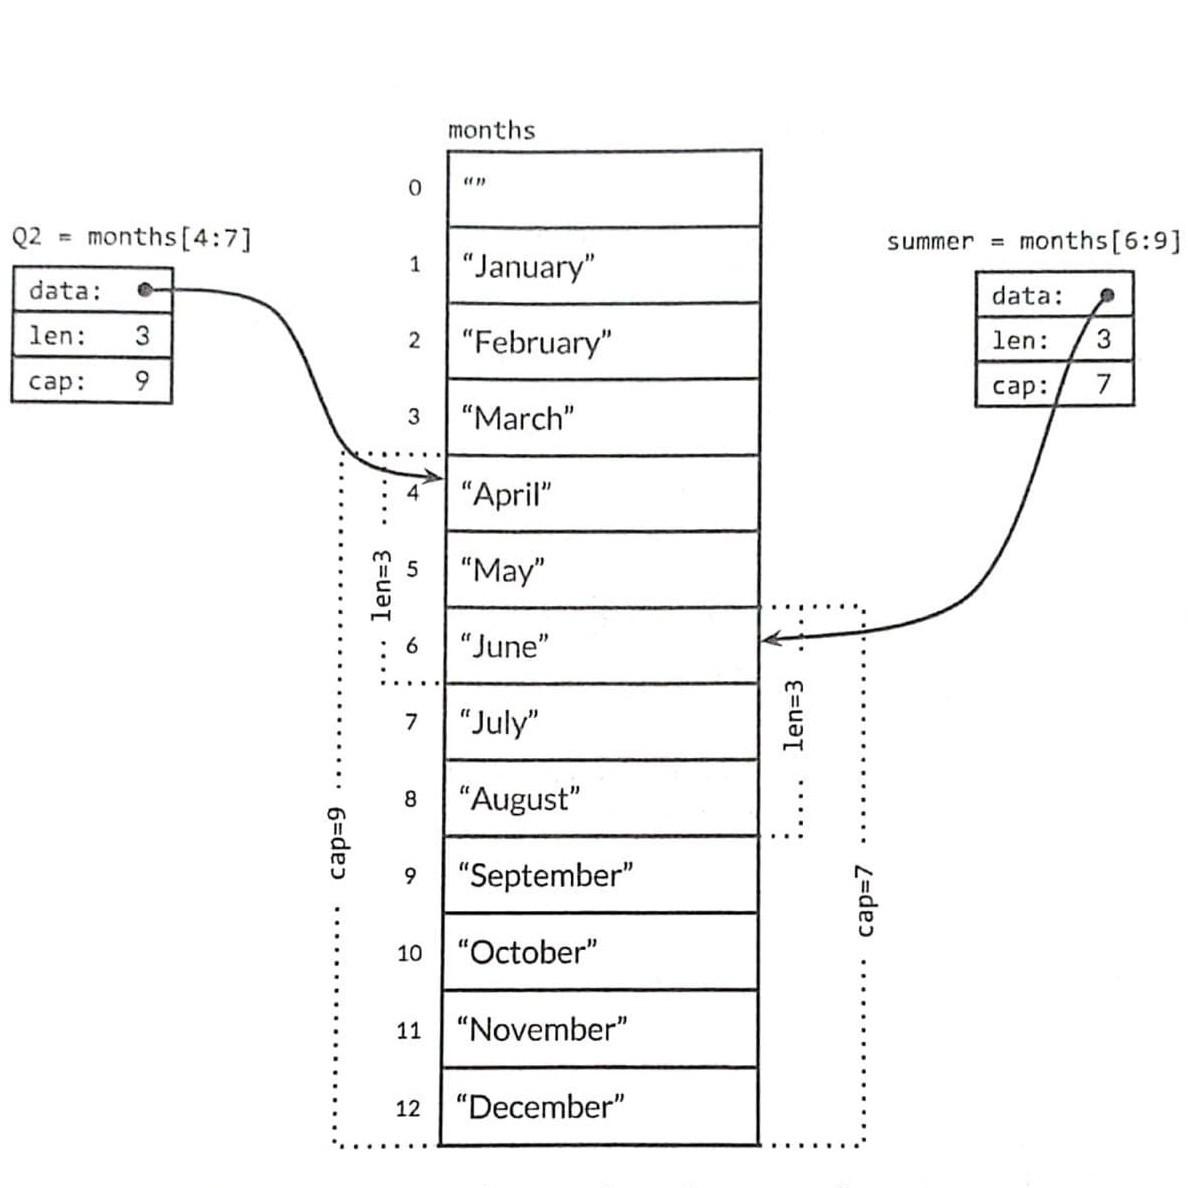
\includegraphics[width=0.5\linewidth]{figures/figura3.1}
\end{center}
\begin{lstlisting}[frame=single, label={lst:lstlisting3-2.2}]
Q2 := months[4:7]
summer := months[6:9]
fmt.Println(Q2)
fmt.Println(summer)
\end{lstlisting}
Output:
\begin{lstlisting}[language=bash, frame=L, label={lst:lstlisting3-2.3}]
[%*``*\)April%*''*\) %*``*\)May%*''*\) %*``*\)June%*''*\)]
[%*``*\)June%*''*\) %*``*\)July%*''*\) %*``*\)August%*''*\)]
\end{lstlisting}
Nell'espressione delle slice, andare oltre \verb|cap(s)| si ottiene una situazione di \verb|panic|, ma andare oltre \verb|len(s)| si ottiene l'estensione della slice, quindi il risultato può diventare più ricco di quello di partenza.
\begin{lstlisting}[frame=single, label={lst:lstlisting3-2.4}]
fmt.Println(summer[:20])    // panic: fuori portata

endlessSummer := summer[:5] // estende una slice entro la sua
                            // capacit%*\textit{à}*\)
fmt.Println(endlessSummer)
\end{lstlisting}
Output:
\begin{lstlisting}[language=bash, frame=L, label={lst:lstlisting3-2.5}]
[June July August September October]
\end{lstlisting}
Poiché una slice contiene un puntatore ad un elemento di un array, passare una slice ad una funzione permette alla funzione di modificare gli elementi dell'array sottostante.
In altre parole, copiare una slice vuol dire creare un \textit{alias} per l'array sottostante.

Uno \textit{slice literal} si presenta come un array literal, una sequenza di valori separati da virgole racchiusi in parentesi graffe, con la dimensione non data.
Questo crea implicitamente una variabile array della giusta dimensione e produce una slice che punta ad essa.
Come con gli array literal, gli slice literal possono specificare in ordine i valori, o assegnare esplicitamente loro gli indici, oppure usare un mix dei due stili.

A differenza degli array, le slice non sono confrontabili, quindi non possiamo usare l'operatore \verb|==| per verificare se due slice contengono gli stessi elementi.
Per i tipi di riferimento come puntatori e channel, l'operatore \verb|==| verifica la \textit{reference identity}, cioè se le due entità riferiscono alla stessa cosa.
La scelta più sicura è quella di non permettere in alcun caso il confronto fra slice.

L'unico confronto legale è con \verb|nil|:
\begin{lstlisting}[frame=single, label={lst:lstlisting3-2.6}]
if summer == nil { /* ... */ }
\end{lstlisting}
Il valore zero di un tipo di slice è \verb|nil|.
Una slice nil non ha un array sottostante.
La slice nil ha lunghezza e capacità zero, ma ci sono anche le slice non nil di lunghezza e capacità zero, come \verb|[]int{}|.
Il valore nil di un particolare tipo di slice può essere scritto usando un'espressione di conversione come \verb|[]int(nil)|.

A meno che non sia chiaramente documentato il contrario, le funzioni Go trattano tutte le slice di lunghezza zero allo stesso modo, sia nil che non nil.

La funzione incorporata \verb|make| crea una slice di un tipo di elemento specificato, e di una certa lunghezza e capacità.
L'argomento capacità può essere omesso, nel qual caso si intende uguale alla lunghezza.
\begin{lstlisting}[frame=single, label={lst:lstlisting3-2.7}]
make([]T, len)
make([]T, len, cap) // uguale a make([]T, cap)[:len]
\end{lstlisting}
La funzione \verb|make| crea una variabile array senza nome e ne restituisce una slice;
l'array è accessibile solo attraverso la slice restituita.
Nella prima forma, la slice è una vista dell'intero array.
Nel secondo, la slice è una vista solo dei primi \verb|len| elementi dell'array, ma la sua capacità include l'intero array.
Gli elementi aggiuntivi sono quindi accantonati per una crescita futura della slice.

La funzione built-in \verb|append| aggiunge elementi alle slice.

Di solito non sappiamo se una determinata chiamata ad \verb|append| causerà una riallocazione, quindi non possiamo supporre che la slice originale punti allo stesso array della slice risultante, né che si riferisca a una diversa.
Allo stesso modo, non dobbiamo presumere che le assegnazioni ad elementi della vecchia slice si rifletteranno (o non si rifletteranno) sulla nuova slice.
Di conseguenza, è normale assegnare il risultato di una chiamata ad \verb|append| alla stessa variabile slice il cui valore è stato passato alla chiamata della funzione \verb|append|:
\begin{lstlisting}[frame=single, label={lst:lstlisting3-2.8}]
var runes []rune
for _, r := range %*``*\)Hello, World%*''*\) {
    runes = append(runes, r)
}
fmt.Printf(%*``*\)%q\n%*''*\), runes)
\end{lstlisting}
Output:
\begin{lstlisting}[language=bash, frame=L, label={lst:lstlisting3-2.9}]
[`H' `e' `l' `l' `o' `,' `W' `o' `r' `l' `d']
\end{lstlisting}
\
Inoltre, la funzione \verb|append| ci permette di aggiungere più di un nuovo elemento, o anche una slice intera dello stesso tipo.
\begin{lstlisting}[frame=single, label={lst:lstlisting3-2.10}]
var x []int
x = append(x, 1)
x = append(x, 2, 3)
x = append(x, 4, 5, 6)
x = append(x, x...) // Aggiunge la slice x
fmt.Println(x)
\end{lstlisting}
Output:
\begin{lstlisting}[language=bash, frame=L, label={lst:lstlisting3-2.11}]
[1 2 3 4 5 6 1 2 3 4 5 6]
\end{lstlisting}
Verrà spiegato più in avanti il perché dell'ellissi ``\verb|...|'' nella chiamata alla funzione \verb|append| nell'ultimo esempio.

Una slice può essere usata per implementare uno stack.
Data uno stack di slice inizialmente vuota, possiamo spingere un nuovo valore alla fine della slice con \verb|append|:
\begin{lstlisting}[frame=single, label={lst:lstlisting3-2.12}]
stack = append(stack, v) // push v
\end{lstlisting}
La testa dello stack è l'ultimo elemento:
\begin{lstlisting}[frame=single, label={lst:lstlisting3-2.13}]
top := stack[len(stack)-1] // top dello stack
\end{lstlisting}
e la restrizione dello stack effettuando il pop dell'elemento:
\begin{lstlisting}[frame=single, label={lst:lstlisting3-2.14}]
stack := stack[:len(stack)-1] // pop
\end{lstlisting}
Per rimuovere un elemento dal centro di una slice, conservando l'ordine degli elementi rimanenti, si usa \verb|copy| per far scorrere gli elementi con il numero più alto verso il basso di uno a riempire lo spazio vuoto generato:
\begin{lstlisting}[frame=single, label={lst:lstlisting3-2.15}]
func remove(slice []int, i int) []int {
    copy(slice[i:], slice[i+1:])
    return slice[:len(slice)-1]
}

func main() {
    s := []int{5, 6, 7, 8, 9}
    fmt.Println(remove(s, 2))
}
\end{lstlisting}
Output:
\begin{lstlisting}[language=bash, frame=L, label={lst:lstlisting3-2.16}]
[5 6 8 9]
\end{lstlisting}

\section{Maps}
\label{sec:maps}
%
La tabella hash è una delle più ingegnose e versatili di tutte le strutture dati.
Si tratta di una raccolta non ordinata di coppie chiave/valore in cui tutte le chiavi sono distinte e il valore associato a una determinata chiave può essere recuperato, aggiornato o rimosso utilizzando in media un numero costante di confronti di chiave, non importa quanto grande sia la tabella hash.

In Go, una \textit{map} è un riferimento a una tabella hash, ed è scritto \verb|map[K]V|, dove \verb|K| e \verb|V| sono i tipi delle sue chiavi e dei suoi valori.
Tutte le chiavi in una determinata map sono dello stesso tipo e tutti i valori sono dello stesso tipo, ma le chiavi non devono necessariamente essere dello stesso tipo dei valori.
Il tipo di chiave \verb|K| deve essere comparabile usando \verb|==|, in modo che la map possa verificare se una determinata chiave è uguale a una già all'interno di essa.
Non ci sono restrizioni sul tipo di valore \verb|V|.

La funzione integrata \verb|make| può essere utilizzata per creare una map:
\begin{lstlisting}[label={lst:lstlisting3-3.1}]
ages := make(map[string]int) // map da string a int
\end{lstlisting}
Possiamo anche usare una \textit{map literal} per creare una nuova map popolata da alcune coppie chiave/valore iniziali:
\begin{lstlisting}[frame=single, label={lst:lstlisting3-3.2}]
ages := map[string]int {
    %*``*\)alice%*''*\):   31,
    %*``*\)charlie%*''*\): 34,
}
\end{lstlisting}
Ciò equivale a
\begin{lstlisting}[frame=single, label={lst:lstlisting3-3.3}]
ages := make(map[string]int)
ages[%*``*\)alice%*''*\)] = 31
ages[%*``*\)charlie%*''*\)] = 34
\end{lstlisting}
quindi un'espressione alternativa per una nuova map vuota è \verb|map[string]int{}|.

Gli elementi della map sono accessibili attraverso la consueta notazione:
\begin{lstlisting}[frame=single, label={lst:lstlisting3-3.4}]
ages[%*``*\)alice%*''*\)] = 32
fmt.Println(ages[%*``*\)alice%*''*\)])
\end{lstlisting}
Output:
\begin{lstlisting}[language=bash, frame=L, label={lst:lstlisting3-3.5}]
32
\end{lstlisting}
e rimosso con la funzione integrata \verb|delete|:
\begin{lstlisting}[language=go, frame=single, label={lst:lstlisting3-3.6}]
delete(ages, %*``*\)alice%*''*\)) // rimuovere elemento et%*\textit{à}*\)[%*``*\)alice%*''*\)]
\end{lstlisting}
Tutte le operazioni sono sicure anche se l'elemento non è nella map;
una ricerca di una chiave che non è presente nella map restituisce il valore zero per il suo tipo, così, per esempio, il seguente codice funziona anche quando ``bob'' non è ancora una chiave della map perché il valore di \verb|ages["bob"]| sarà \verb|0|.
\begin{lstlisting}[frame=single, label={lst:lstlisting3-3.7}]
ages[%*``*\)bob%*''*\)]++
\end{lstlisting}
Ma un elemento della map non è una variabile, per cui non si può ottenere il suo indirizzo
\begin{lstlisting}[frame=single, label={lst:lstlisting3-3.8}]
_ = &ages[%*``*\)bob%*''*\)] // compile error: impossibile prendere
                // l'indirizzo di un elemento di map
\end{lstlisting}
Il valore zero per una map è \verb|nil|, cioè un riferimento a nessuna tabella hash.
\begin{lstlisting}[frame=single, label={lst:lstlisting3-3.9}]
var ages map[string]int
fmt.Println(ages == nil)
fmt.Println(len(ages) == 0)
\end{lstlisting}
Output:
\begin{lstlisting}[language=bash, frame=L, label={lst:lstlisting3-3.10}]
true
true
\end{lstlisting}
La maggior parte delle operazioni sulle map, inclusi i cicli di ricerca, \verb|delete|, \verb|len| e \verb|range|, sono sicure da eseguire su una map di riferimento nil, poiché si comporta come una mappa vuota.
Ma la memorizzazione di una map nil provoca panic:
\begin{lstlisting}[frame=single, label={lst:lstlisting3-3.11}]
ages[%*``*\)carol%*''*\)] = 21 // panic: assegnazione ad una map nil
\end{lstlisting}
È necessario allocare la map prima di poter memorizzare in esso coppie chiave/valore.
In particolare, se si vuole sapere se una chiave è presente nella map, allora si può effettuare una chiamata:
\begin{lstlisting}[frame=single, label={lst:lstlisting3-3.12}]
age, ok = ages[%*``*\)bob%*''*\)]
\end{lstlisting}
In cui il primo valore contiene il valore associato alla chiave \verb|bob| nella map (se presente), mentre il secondo contiene un valore booleano che indica se la chiave è presente o meno nella map.

Come nelle slice, le map non possono essere confrontate fra loro;
l'unico confronto legale è con \verb|nil|.

\section{Struct}
\label{sec:struct}
%
Una \textit{struct} è un tipo di dati aggregato che raggruppa insieme zero o più valori denominati di tipi arbitrari in una singola entità.
Ogni valore è detto \textit{campo}.

Queste due istruzioni dichiarano un tipo di struct chiamato \verb|Employee| e una variabile chiamata \verb|dilbert| che è un'istanza di un \verb|Employee|:
\begin{lstlisting}[frame=single, label={lst:lstlisting3-4.1}]
type Employee struct {
    ID 	      int
    Name      string
    Address   string
    DoB       time.Time
    Position  string
    Salary    int
    ManagerID int
}

var dilbert Employee
\end{lstlisting}
I singoli campi di \verb|dilbert| sono accessibili usando la notazione a punti (\verb|dilbert.Name| e \verb|dilbert.DoB|).
Poiché \verb|dilbert| è una variabile, anche i suoi campi sono variabili, quindi possiamo assegnare ad un campo:
\begin{lstlisting}[frame=single, label={lst:lstlisting3-4.2}]
dilbert.Salary -= 5000
\end{lstlisting}
o prendere il suo indirizzo e accedervi tramite un puntatore:
\begin{lstlisting}[frame=single, label={lst:lstlisting3-4.3}]
position := &dilbert.Position
*position = %*``*\)Senior %*''*\) + *position
\end{lstlisting}
La notazione a punti funziona anche con un puntatore a una struct:
\begin{lstlisting}[frame=single, label={lst:lstlisting3-4.4}]
var employeeOfTheMonth *Employee = &dilbert
employeeOfTheMonth.Position += %*``*\) (proactive team player)%*''*\)
\end{lstlisting}
Dove l'ultima istruzione è equivalente a
\begin{lstlisting}[frame=single, label={lst:lstlisting3-4.5}]
(*employeeOfTheMonth).Position += %*``*\) (proactive team player)%*''*\)
\end{lstlisting}
I campi sono di solito scritti uno per riga, con il nome del campo che precede il suo tipo, ma i campi consecutivi dello stesso tipo possono essere combinati, come con \verb|Name| e \verb|Address| qui:
\begin{lstlisting}[frame=single, label={lst:lstlisting3-4.6}]
type Employee struct {
    ID            int
    Name, Address string
    DoB           time.Time
    Position      string
    Salary        int
    ManagerID     int
}
\end{lstlisting}
Un tipo di struct denominato \verb|S| non può dichiarare un campo dello stesso tipo \verb|S|: un valore aggregato non può contenere se stesso.
Ma \verb|S| può dichiarare un campo del tipo di puntatore \verb|*S|, che ci permette di creare struct di dati ricorsive come liste concatenate e alberi.
Questo è illustrato nel codice qui sotto, che utilizza un albero binario per implementare un ordinamento di inserimento:
\begin{lstlisting}[frame=single, label={lst:lstlisting3-4.7}]
type tree struct {
    value       int
    left, right *tree
}

// Sorts ordina i valori in posizione.
func Sort(values []int) {
    var root *tree
    for _, v := range values {
        root = add(root, v)
    }
    appendValues(values[:0], root)
}

// appendValues aggiunge gli elementi di t ai valori
// in ordine e restituisce la slice risultante.
func appendValues(values []int, t *tree) []int {
    if t != nil {
        values = appendValues(values, t.left)
        values = append(values, t.value)
        values = appendValues(values, t.right)
    }
    return values
}

func add(t *tree, value int) *tree {
    if t == nil {
        // Equivalente a ritornare &tree{value:value}
        t = new(tree)
        t.value = value
        return t
    }
    if value < t.value {
        t.left = add(t.left, value)
    } else {
        t.right = add(t.right, value)
    }
    return t
}
\end{lstlisting}
Il valore zero per una struct è composto dai valori zero di ciascuno dei suoi campi.

Il tipo di struct senza campi è chiamato \textit{empty struct}, scritto \verb|struct{}|.

\subsection{Struct literal}
\label{subsec:struct_literal}%
Un valore di un tipo di struttura può essere scritto usando una \textit{struct literal} che specifica i valori per i suoi campi.
\begin{lstlisting}[frame=single, label={lst:lstlisting3-4-1.1}]
type Point struct { X, Y int }

p := Point{1, 2}
\end{lstlisting}
Ci sono due forme di struct literal.
La prima forma, mostrata sopra, richiede che sia specificato un valore per \textit{ogni} campo nell'ordine giusto.
Rende il codice fragile se l'insieme dei campi dovesse poi crescere o essere riordinato.
Di conseguenza, questa forma tende ad essere usata solo all'interno del pacchetto che definisce il tipo di struct, o con tipi di struct più piccoli per i quali esiste un'ovvia convenzione di ordinamento dei campi, come \verb|image.Point{x, y}| o \verb|color.RGBA{red, green, blue, alpha}|.

Più spesso, viene usata la seconda forma, in cui un valore di struct viene inizializzato elencando alcuni o tutti i nomi dei campi e i loro valori corrispondenti.
Se un campo è omesso in questo tipo di literal, viene impostato al valore zero per il suo tipo.

I valori di struct possono essere passati come argomenti alle funzioni e restituiti da esse.
Per esempio, questa funzione scala un ``Punto'' di un fattore specificato:
\begin{lstlisting}[frame=single, label={lst:lstlisting3-4-1.2}]
func Scale(p Point, factor int) Point {
    return Point{p.X * factor, p.Y * factor}
}

fmt.Println(Scale(Point{1, 2}, 5))
\end{lstlisting}
Output:
\begin{lstlisting}[language=bash, frame=L, label={lst:lstlisting3-4-1.3}]
{5 10}
\end{lstlisting}
Per efficienza, la struct più grande è solitamente passata a o restituita da funzioni indirettamente usando un puntatore
\begin{lstlisting}[frame=single, label={lst:lstlisting3-4-1.4}]
func Bonus(e *Employee, percent int) int {
    return e.Salary * percent / 100
}
\end{lstlisting}
e questo è necessario se la funzione deve modificare il suo argomento, poiché in un linguaggio call-by-value come Go, la funzione chiamata riceve solo una copia di un argomento, non un riferimento all'argomento originale.

\subsection{Confronto tra struct}
\label{subsec:confronto_tra_struct}%
Se tutti i campi di una struct sono comparabili, la struct stessa è comparabile, quindi due espressioni di quel tipo possono essere confrontate usando \verb|==| o \verb|!=|.
L'operazione \verb|==| confronta i campi corrispondenti delle due struct in ordine, quindi le due espressioni stampate qui sotto sono equivalenti:
\begin{lstlisting}[frame=single, label={lst:lstlisting3-4-2.1}]
type Point struct { X, Y int }

p := Point{1, 2}
q := Point{2, 1}
fmt.Println(p.X == q.X && p.Y == q.Y)
fmt.Println(p == q)
\end{lstlisting}
Output:
\begin{lstlisting}[language=bash, frame=L, label={lst:lstlisting3-4-2.2}]
false
false
\end{lstlisting}

\subsection{Struct embedding e campi anonimi}
\label{subsec:struct_embedding_e_campi_anonimi}%
Un insolito meccanismo \textit{struct embedding} ci permette di usare un tipo di struct detto \textit{campo anonimo} di un altro tipo di struct, fornendo una comoda scorciatoia sintattica in modo che una semplice espressione puntiforme come \verb|x.f| possa rappresentare una catena di campi come \verb|x.d.e.f|.
Dati le seguenti struct:
\begin{lstlisting}[frame=single, label={lst:lstlisting3-4-3.1}]
type Circle struct {
    X, Y, Radius int
}

type Wheel struct {
    X, Y, Radius, Spokes int
}
\end{lstlisting}
conviene raccogliere i campi uguali a individuare una nuova struct
\begin{lstlisting}[frame=single, label={lst:lstlisting3-4-3.2}]
type Point struct {
    X, Y int
}
type Circle struct {
    Center Point
    Radius int
}

type Wheel struct {
    Circle Circle
    Spokes int
}
\end{lstlisting}
L'applicazione diventerebbe più chiara, ma questo cambiamento renderebbe anche l'accesso ai campi di ``Wheel'' più prolisso:
\begin{lstlisting}[frame=single, label={lst:lstlisting3-4-3.3}]
var w Wheel
w.Circle.Center.X = 8
w.Circle.Center.Y = 8
w.Circle.Radius = 5
w.Spokes = 20
\end{lstlisting}
Go ci permette di dichiarare un campo con un tipo ma senza nome;
tali campi sono chiamati \textit{campi anonimi}.
Il tipo di campo deve essere un tipo con nome o un puntatore a un tipo con nome.
Sotto, \verb|Circle| e \verb|Wheel| hanno un campo anonimo ciascuno.
Diciamo che un \verb|Point| è \textit{incorporato} all'interno di \verb|Circle|, e un \verb|Circle| è incorporato all'interno di \verb|Wheel|.
\begin{lstlisting}[frame=single, label={lst:lstlisting3-4-3.4}]
type Circle struct {
    Point
    Radius int
}

type Wheel struct {
    Circle
    Spokes int
}
\end{lstlisting}
Grazie all'incorporazione, possiamo fare riferimento ai nomi alle foglie dell'albero implicito senza dare i nomi intermedi:
\begin{lstlisting}[frame=single,label={lst:lstlisting3-4-3.5}]
var w Wheel
w.X = 8	     // equivalente a w.Circle.Point.X = 8
w.Y = 8	     // equivalente a w.Circle.Point.Y = 8
w.Radius = 5 // equivalente a w.Circle.Radius = 5
w.Spokes = 20
\end{lstlisting}
Poiché i campi ``anonimi'' hanno nomi impliciti, non è possibile avere due campi anonimi dello stesso tipo perché in tal caso i loro nomi entrerebbero in conflitto.

Il tipo struct esterno guadagna non solo i campi del tipo embedded ma anche i suoi metodi.
Questo meccanismo è il modo principale in cui i comportamenti degli oggetti complessi sono composti da quelli più semplici.
La \textit{composizione} è centrale per la programmazione orientata agli oggetti in Go.




    \chapter{Funzioni}
    \label{ch:funzioni}%
    Una funzione ci permette di avvolgere una sequenza di istruzioni come un'unità che può essere chiamata da altrove in un programma, anche più volte.
Le funzioni permettono di suddividere un grande lavoro in parti più piccole.
Una funzione nasconde i dettagli della sua implementazione ai suoi utenti.
Per tutti questi motivi, le funzioni sono una parte critica di tutto il linguaggio di programmazione.


\section{Dichiarazione di funzione}
\label{sec:dichiarazione_di_funzione}%
Una dichiarazione di funzione ha un nome, un elenco di parametri, un elenco opzionale di risultati e un corpo:
\begin{lstlisting}[label={lst:lstlisting4-1.1}]
func nome(elenco-parametri) (elenco-risultati) {
   corpo
}
\end{lstlisting}
L'elenco dei parametri specifica i nomi e i tipi dei \textit{parametri} della funzione, che sono la variabile locale i cui valori o \textit{argomenti} sono forniti dal chiamante.
L'elenco dei risultati specifica i tipi di valori restituiti dalla funzione.
Se la funzione restituisce un risultato senza nome o nessun risultato, le parentesi sono facoltative e di solito omesse.
Omettere la lista dei risultati vuol dire che la funzione non restituisce alcun valore ed è chiamata solo per i suoi effetti.

Una sequenza di parametri o risultati dello stesso tipo può essere scomposta in modo che il tipo stesso sia scritto solo una volta.

In seguito vengono presentati quattro modi per dichiarare una funzione con due parametri e un risultato, tutti di tipo \verb|int|.
L'identificatore vuoto può essere utilizzato per sottolineare che un parametro non è utilizzato.
\begin{lstlisting}[frame=single, label={lst:lstlisting4-1.2}]
func add(x int, y int) { return x + y }
func sub(x, y int) (z int) { z = x - y; return }
func first(x int, _ int) int { return x }
func zero(int, int) int { return 0 }

fmt.Printf(%*``*\)%T\n%*''*\), add)
fmt.Printf(%*``*\)%T\n%*''*\), sub)
fmt.Printf(%*``*\)%T\n%*''*\), first)
fmt.Printf(%*``*\)%T\n%*''*\), zero)
\end{lstlisting}
Output:
\begin{lstlisting}[language=bash, frame=L, label={lst:lstlisting4-1.3}]
func(int, int) int
func(int, int) int
func(int, int) int
func(int, int) int
\end{lstlisting}
Il tipo di una funzione è talvolta detta la sua \textit{firma}.
Due funzioni hanno lo stesso tipo o firma se hanno la stessa sequenza di tipi di parametri e la stessa sequenza di tipi di risultato.
I nomi dei parametri e dei risultati non influenzano il tipo, né il fatto che siano stati dichiarati o meno utilizzando la forma fattorizzata.

Gli argomenti vengono passati \textit{per valore}, quindi la funzione riceve una copia di ogni argomento;
le modifiche alla copia non influenzano il chiamante.
Tuttavia, se l'argomento contiene un qualche tipo di riferimento, come un puntatore, una slice, una map, una funzione o un channel, allora il chiamante può essere influenzato da qualsiasi modifica che la funzione apporta \textit{indirettamente} alle variabili cui fa riferimento l'argomento.

Si può occasionalmente incontrare una dichiarazione di funzione senza un corpo, indicando che la funzione è implementata in un linguaggio diverso da Go.
Tale dichiarazione definisce la firma della funzione.
\begin{lstlisting}[frame=single, label={lst:lstlisting4-1.4}]
package math

func Sin(x float64) float64 // implementato in linguaggio
                            // assembly p.e.
\end{lstlisting}


\section{Valori di ritorno multipli}
\label{sec:valori_di_ritorno_multipli}%
Una funzione può restituire più di un risultato.
Il risultato della chiamata di una funzione multi-valore è una tupla di valori.
Il chiamante della funzione deve esplicitare l'assegnazione dei valori alle variabili nel caso una di esse verrà in seguito usata.
\begin{lstlisting}[frame=single, label={lst:lstlisting4-3.1}]
links, err := findLinks(url)
\end{lstlisting}
Per ignorare uno dei valori, assegnare uno di essi agli identificatori blank:
\begin{lstlisting}[frame=single, label={lst:lstlisting4-3.2}]
links, _ := findLinks(url) // gli errori sono ignorati
\end{lstlisting}
Il risultato di una chiamata multi-valore può essere a sua volta restituito da una funzione di chiamata (multi-valori), come in questa funzione:
\begin{lstlisting}[frame=single, label={lst:lstlisting4-3.3}]
func findLiksLog(url string) ([]string, error) {
    log.Printf(%*``*\)findLinks %s%*''*\), url)
    return findLinks(url)
}
\end{lstlisting}
Una chiamata multi-valore può apparire come unico argomento quando si chiama una funzione con più parametri.
Anche se raramente usato nel codice di produzione, questa caratteristica è a volte conveniente durante il debug in quanto ci permette di stampare tutti i risultati di una chiamata utilizzando una singola istruzione.
Le due istruzioni di stampa qui sotto hanno lo stesso effetto.
\begin{lstlisting}[frame=single, label={lst:lstlisting4-3.4}]
log.Println(findLinks(url))

links, err := findLinks(url)
log.Println(links, err)
\end{lstlisting}
In una funzione con risultati denominati, gli operandi di un'istruzione return possono essere omessi.
Questo è chiamato a \textit{bare return}.
\begin{lstlisting}[frame=single, label={lst:lstlisting4-3.5}]
func CountWordsAndImages(url string) (words, images int,
                                                err error) {
    resp, err := http.Get(url)
    if err != nil {
        return
    }
    doc, err := html.Parse(resp.Body)
    resp.Body.Close()
    if err != nil {
        err = fmt.Errorf(%*``*\)parsing HTML: %s%*''*\), err)
        return
    }
    words, images = countWordAndImages(doc)
    return
}

func countWordsAndImages(n *html.Node) (words, images int) {
    /* ... */
}
\end{lstlisting}
Un brave return è un modo abbreviato per restituire ciascuna delle variabili di risultato nominate in ordine, quindi nella funzione sopra, ogni dichiarazione di ritorno è equivalente a:
\begin{lstlisting}[frame=single, label={lst:lstlisting4-3.6}]
return word, images, err
\end{lstlisting}
In funzioni come questa, con molte istruzioni di ritorno e diversi risultati, i bare return possono ridurre la duplicazione del codice, ma raramente rendono il codice più facile da capire.


\section{Errori}
\label{sec:errori}%
L'approccio di Go lo distingue da molti altri linguaggi in cui i fallimenti sono segnalati usando \textit{eccezioni}, non valori ordinari.
Anche se Go ha un meccanismo di eccezione di sorta, è usato solo per segnalare errori veramente inaspettati che indicano un bug, non gli errori di routine che un programma robusto dovrebbe aspettarsi.

Una funzione per la quale il fallimento è un comportamento atteso restituisce un risultato aggiuntivo, convenzionalmente l'ultimo.
Se il fallimento ha una sola possibile causa, il risultato è un booleano, di solito chiamato \verb|ok|.
Più spesso il fallimento può avere una varietà di cause per le quali il chiamante avrà bisogno di una spiegazione.
In tali casi, il tipo di risultato aggiuntivo è \verb|error| (un tipo di interfaccia).

La ragione di questo progetto è che le eccezioni tendono ad impigliare la descrizione di un errore con il flusso di controllo richiesto per gestirlo, spesso portando ad un risultato indesiderato: gli errori di routine vengono segnalati all'utente finale sotto forma di una traccia di stack incomprensibile, pieno di informazioni sulla struttura del programma, ma privo di contesto intelligibile su ciò che è andato storto.

Al contrario, i programmi Go usano meccanismi di controllo di flusso ordinari come \verb|if| e \verb|return| per rispondere agli errori.
Questo stile richiede innegabilmente una maggiore attenzione alla logica di gestione degli errori.


\section{Valori di funzione}
\label{sec:valori_di_funzione}%
Le funzioni sono \textit{valori di prima classe} in Go: come altri valori, i valori di funzione hanno tipi, e possono essere assegnati a variabili o passati a o restituiti da funzioni.
Un valore di funzione può essere chiamato come qualsiasi altra funzione.
\begin{lstlisting}[frame=single, label={lst:lstlisting4-5.1}]
func square(n int) int { return n * n }
func negative(n int) int { return -n }
func product(m, n int) int { return m * n }

f := square
fmt.Println(f(3))

f = negative
fmt.Println(f(3))
fmt.Printf(%*``*\)%T\n%*''*\), f)

f = product // compile error: non pu%*\textit{ò}*\) assegnare
            // func(int, int) int a func(int) int
\end{lstlisting}
Output:
\begin{lstlisting}[language=bash, frame=L, label={lst:lstlisting4-5.2}]
9
-3
func(int) int
\end{lstlisting}
Il valore zero di un tipo di funzione è \verb|nil|.
Chiamare un valore di funzione \verb|nil| provoca il panic:
\begin{lstlisting}[frame=single, label={lst:lstlisting4-5.3}]
var f func(int) int
f(3) // panic: chiamata ad una funzione nil
\end{lstlisting}
I valori di funzione possono essere confrontati con ``nil'':
\begin{lstlisting}[frame=single, label={lst:lstlisting4-5.4}]
var f func(int) int
if f != nil {
    f(3)
}
\end{lstlisting}
ma non sono paragonabili, quindi non sono confrontati tra loro o utilizzati come chiavi in una mappa.

I valori delle funzioni ci permettono di parametrizzare le nostre funzioni non solo sui dati, ma anche sul comportamento.
Le librerie standard contengono molti esempi.
Per esempio, \verb|strings.Map| applica una funzione ad ogni carattere di una stringa, unendo i risultati per creare un'altra stringa.
\begin{lstlisting}[frame=single, label={lst:lstlisting4-5.5}]
func add1(r rune) rune { return r + 1 }

fmt.Println(strings.Map(add1, %*``*\)HAL-9000%*''*\)))
fmt.Println(strings.Map(add1, %*``*\)VMS%*''*\)))
fmt.Println(strings.Map(add1, %*``*\)Admix%*''*\)))
\end{lstlisting}
Output:
\begin{lstlisting}[language=bash, frame=L, label={lst:lstlisting4-5.6}]
IBM.:111
WNT
Benjy
\end{lstlisting}


\section{Funzioni anonime}
\label{sec:funzioni_anonime}%
Le funzioni con nome possono essere dichiarate solo a livello di pacchetto, ma possiamo usare una \textit{function literal} per denotare un valore di funzione all'interno di qualsiasi espressione.
Una funzione literal è scritta come una dichiarazione di funzione, ma senza un nome che segue la parola chiave \verb|func|.
È un'espressione, e il suo valore è detto \textit{funzione anonima}.

I function literal permettono di definire una funzione nel loro punto d'uso:
\begin{lstlisting}[frame=single, label={lst:lstlisting4-6.1}]
strings.Map(func(r rune) rune { return r + 1 }, %*``*\)HAL-9000%*''*\))
\end{lstlisting}
Ancora più importante, le funzioni definite in questo modo hanno accesso all'intero ambiente lessicale, quindi la funzione interna può riferirsi alle variabili dalla funzione che la racchiude:
\begin{lstlisting}[frame=single, label={lst:lstlisting4-6.2}]
func squares() func() int {
    var x int
    return func() int {
        x++
        return x * x
    }
}
\end{lstlisting}
\begin{lstlisting}[frame=single, label={lst:lstlisting4-6.3}]
func main() {
    f := squares()
    fmt.Println(f())
    fmt.Println(f())
    fmt.Println(f())
    fmt.Println(f())
}
\end{lstlisting}
Output:
\begin{lstlisting}[language=bash, frame=L, label={lst:lstlisting4-6.4}]
1
4
9
16
\end{lstlisting}
La funzione \verb|squares| restituisce un'altra funzione, di tipo \verb|func() int|.
La prima chiamata a \verb|squares| crea una variabile locale \verb|x| e restituisce una funzione anonima che, ogni volta che viene chiamata, incrementa \verb|x| e ne restituisce il suo quadrato.
Una seconda chiamata a \verb|squares| crea una seconda variabile \verb|x| e restituisce una nuova funzione anonima che incrementa quella variabile.

L'esempio \verb|squares| dimostra che i valori di funzione non sono solo codice ma possono avere stato.
La funzione interna anonima può accedere e aggiornare le variabili locali della funzione \verb|squares| che la racchiude.
Questi riferimenti di variabili nascoste sono il motivo per cui le funzioni si classificano come tipi di riferimento e il perché i valori di funzione non sono comparabili.
I valori di funzione come questi sono effettuati facendo uso di una tecnica detta \textit{closure} ed i programmatori di Go usano spesso questo termine per i valori di funzione.

Quando una funzione anonima richiede la ricorsione, bisogna prima dichiarare una variabile e quindi assegnare la funzione anonima a quella variabile.
Se i due passi sono combinati nella dichiarazione (con un'istruzione \verb|:=|), la function literal non rientrerebbe nell'ambito della variabile, quindi non avrebbe modo di chiamarsi ricorsivamente.


\section{Funzioni variadic}
\label{sec:funzioni_variadic}%
Una \textit{funzione variadic} può essere chiamata con un numero variabile di argomenti.
Gli esempi più familiari sono \verb|fmt.Printf| e le sue varianti.
\verb|Printf| richiede un argomento fisso all'inizio, quindi accetta qualsiasi numero di argomenti successivi.

Per dichiarare una funzione variadic, il tipo del parametro finale è preceduto da un ellissi, ``\verb|...|'', che indica che la funzione può essere chiamata con qualsiasi numero di argomenti di questo tipo.
\begin{lstlisting}[frame=single, label={lst:lstlisting4-7.1}]
func sum(vals ...int) int {
   total := 0
   for _, val := range vals {
      total += val
   }
   return total
}
\end{lstlisting}
La funzione \verb|sum| restituisce la somma di zero o più argomenti \verb|int|.
All'interno del corpo della funzione, il tipo di \verb|vals| è una slice \verb|[]int|.
Quando si invoca \verb|sum|, qualunque numero di valori può essere fornito come parametro \verb|vals|.
\begin{lstlisting}[frame=single, label={lst:lstlisting4-7.2}]
fmt.Println(sum())
fmt.Println(sum(3))
fmt.Println(sum(1, 2, 3, 4))
\end{lstlisting}
Output:
\begin{lstlisting}[language=bash, frame=L, label={lst:lstlisting4-7.3}]
0
3
10
\end{lstlisting}
Implicitamente, il chiamante alloca un array, copia gli argomenti in esso, e passa una slice dell'intero array alla funzione.
L'ultima chiamata dell'ultimo esempio si comporta come la chiamata del seguente esempio, in cui si mostra come invocare una funzione variadic quando gli argomenti sono già in una slice: si deve posizionare un ellissi dopo l'argomento finale.
\begin{lstlisting}[frame=single, label={lst:lstlisting4-7.4}]
values := []int{1, 2, 3, 4}
fmt.Println(sum(values...))
\end{lstlisting}
Output:
\begin{lstlisting}[language=bash, frame=L, label={lst:lstlisting4-7.5}]
10
\end{lstlisting}
Sebbene il parametro \verb|...int| si comporti come una slice all'interno del corpo della funzione, il tipo di una funzione variadic è distinto dal tipo di una funzione con un parametro slice ordinario.
\begin{lstlisting}[frame=single, label={lst:lstlisting4-7.6}]
func f(...int) {}
func g([]int) {}

fmt.Printf(%*``*\)%T\n%*''*\), f)
fmt.Printf(%*``*\)%T\n%*''*\), g)
\end{lstlisting}
Output:
\begin{lstlisting}[language=bash, frame=L, label={lst:lstlisting4-7.7}]
func(...int)
func([]int)
\end{lstlisting}


\section{Chiamate con funzione differita}
\label{sec:chiamate_con_funzione_differita}%
Sintatticamente, un'istruzione \verb|defer| è una funzione ordinaria o una chiamata di metodo preceduta dalla parola chiave \verb|defer|.
Le espressioni di funzione e argomento vengono valutate quando l'istruzione viene eseguita, ma la chiamata effettiva viene \textit{differita} fino a quando la funzione che contiene l'istruzione \verb|defer| non è terminata, sia che si tratti normalmente di eseguire un'istruzione return, o anormalmente, dal panic.
Qualsiasi numero di chiamate può essere differito;
vengono eseguite al contrario dell'ordine in cui sono state differite.

Una dichiarazione di \verb|defer| viene spesso utilizzata con operazioni associate come aprire e chiudere, connettersi e disconnettersi o bloccare e sbloccare per garantire che le risorse vengano rilasciate in tutti i casi, indipendentemente dalla complessità del flusso di controllo.
Il posto giusto per un'istruzione \verb|defer| che rilascia una risorsa è immediatamente dopo che la risorsa è stata acquisita con successo.
\begin{lstlisting}[frame=single, label={lst:lstlisting4-8.1}]
package ioutil

func ReadFile(filename string) ([]byte, error) {
    f, err := os.Open(filename)
    if err != nil {
        return nil, err
    }
    defer f.Close()
    return ReadAll(f)
}
\end{lstlisting}
\begin{lstlisting}[frame=single, label={lst:lstlisting4-8.2}]
var mu sync.Mutex
var m = make(map[string]int)

func lookup(key string) int {
    mu.Lock()
    defer mu.Unlock()
    return m[key]
}
\end{lstlisting}
\begin{lstlisting}[frame=single, label={lst:lstlisting4-8.3}]
func bigSlowOperation() {
    defer trace(%*``*\)bigSlowOperation%*''*\))() // non si dimentichino le
                                     // parentesi extra per
                                     // avviare la funzione
    time.Sleep(10 * time.Second)     // si simula un'operazione
                                     // lenta
}

func trace(msg string) func() {
    start := time.Now()
    log.Printf(%*``*\)enter %s%*''*\), msg)
    return func() {
        log.Printf(%*``*\)exit %s (%s)%*''*\), msg, time.Since(start))
    }
}
\end{lstlisting}
Output:
\begin{lstlisting}[language=bash, frame=L, label={lst:lstlisting4-8.4}]
2022/03/05 18:46:39 enter bigSlowOperation
2022/03/05 18:46:49 exit bigSlowOperation (10.000589217s)
\end{lstlisting}
Le funzioni differite vengono eseguite \textit{dopo} che le istruzioni di ritorno hanno aggiornato le variabili dei risultati della funzione.
Poiché una funzione anonima può accedere alle variabili della sua funzione di racchiudimento, inclusi i risultati denominati, una funzione anonima differita può osservare i risultati della funzione.
\begin{lstlisting}[frame=single, label={lst:lstlisting4-8.5}]
func double(x int) (result int) {
    defer func() { fmt.Printf(%*``*\)double(%d) = %d\n%*''*\), x, result) }()
    return x + x
}

func triple(x int) (result int) {
    defer func() { result += x }()
    return double(x)
}

func main() {
    fmt.Println(triple(4))
}
\end{lstlisting}
Output:
\begin{lstlisting}[language=bash, frame=L, label={lst:lstlisting4-8.6}]
double(4) = 8
12
\end{lstlisting}


\section{Panic}
\label{sec:panic}%
Il sistema di tipo di Go cattura gli errori al momento della compilazione, ma altri, come l'accesso all'array out-of-bounds o il puntatore nil, la dereferenza, richiedono controlli al momento dell'esecuzione.
Quando la routine Go rileva questi errori, lancia il \verb|panic|.

Durante un tipico panic, l'esecuzione normale si ferma, tutte le chiamate di funzione differite vengono eseguite e il programma si blocca con un messaggio di log.
Questo messaggio di log include il valore di panic, che di solito è un messaggio di errore di qualche tipo, e, per ogni goroutine, una traccia di stack che mostra la pila di chiamate di funzione che erano attive al momento del panico.
Questo messaggio di log ha spesso abbastanza informazioni per diagnosticare la causa principale del problema senza eseguire di nuovo il programma, quindi dovrebbe sempre essere incluso in una segnalazione di bug su un programma in preda al panic.




    \chapter{Metodi}
    \label{ch:metodi}%
    Dall'inizio degli anni 90, la programmazione orientata agli oggetti (OOP) è stata il paradigma di programmazione dominante nell'industria e nell'istruzione, e quasi tutti i linguaggi ampiamente utilizzati sviluppati da allora hanno offerto supporto a questo approccio.
Go non fa eccezione.

Anche se non esiste una definizione universalmente accettata di programmazione orientata agli oggetti, per i nostri scopi, un \textit{oggetto} è semplicemente un valore o una variabile che ha metodi, e un \textit{metodo} è una funzione associata a un particolare tipo.
Un programma orientato agli oggetti è un programma che utilizza metodi per esprimere le proprietà e le operazioni di ogni struttura dati in modo che i client non debbano accedere direttamente alla rappresentazione dell'oggetto.


\section{Dichiarazioni dei metodi}
\label{sec:dichiarazioni_dei_metodi}%
Un metodo viene dichiarato con una variante della dichiarazione di funzione ordinaria in cui viene visualizzato un parametro aggiuntivo prima del nome della funzione.
Il parametro attribuisce la funzione al tipo di quel parametro.
\begin{lstlisting}[frame=single, label={lst:lstlisting5-1.1}]
package geometry

import %*``*\)math%*''*\)

type Point struct{ X, Y float64 }

// Funzione tradizionale
func Distance(p, q Point) float64 {
    return math.Hypot(q.X-p.X, q.Y-p.Y)
}

// stessa cosa, ma come un metodo del tipo Point
func (p Point) Distance(q Point) float64 {
    return math.Hypot(q.X-p.X, q.Y-p.Y)
}
\end{lstlisting}
Il parametro extra \verb|p| è chiamato \textit{ricevitore} del metodo, un'eredità dei primi linguaggi orientati agli oggetti che descrivono il chiamare un metodo come ``inviare un messaggio ad un oggetto''.

Dal momento che il nome del ricevitore sarà spesso utilizzato, è una buona idea scegliere qualcosa di breve e di essere coerenti tra i metodi.
Una scelta comune è la prima lettera del nome del tipo, come \verb|p| per \verb|Point|.

In una chiamata di metodo, l'argomento del ricevitore appare prima del nome del metodo.
Questo corrisponde alla dichiarazione, in cui il parametro receiver appare prima del nome del metodo.
\begin{lstlisting}[frame=single, label={lst:lstlisting5-1.2}]
p := Point{1, 2}
q := Point{4, 6}
fmt.Println(Distance(p, q)) // chiamata di funzione
fmt.Println(q.Distance(q))  // chiamata del metodo
\end{lstlisting}
Output:
\begin{lstlisting}[language=bash, frame=L, label={lst:lstlisting5-1.3}]
5
5
\end{lstlisting}
Non c'è conflitto tra le due dichiarazioni di funzioni chiamate \verb|Distance|.
La prima dichiara una funzione a livello di pacchetto chiamata \verb|geometry.Distance|.
La seconda dichiara un metodo del tipo \verb|Point|, quindi il suo nome è \verb|Point.Distance|.

L'espressione \verb|p.Distance| è detta \textit{selettore} perché seleziona il metodo \verb|Distance| appropriato per il ricevitore \verb|p| di tipo \verb|Point|.
I selettori sono anche usati per selezionare i campi dei tipi di struct, come in \verb|p.X|.
Poiché i metodi e i campi abitano lo stesso namespace, dichiarare un metodo \verb|X| sul tipo di struct \verb|Point| sarebbe ambiguo e il compilatore lo rifiuterebbe.

Poiché ogni tipo ha il suo spazio dei nomi per i metodi, possiamo usare il nome \verb|Distance| per altri metodi purché appartengano a diversi tipi.
Definiamo un tipo \verb|Path| assegnandoli anche un metodo \verb|Distance|.
\begin{lstlisting}[frame=single, label={lst:lstlisting5-1.4}]
// Un Path collega i punti con linee rette.
type Path []Point

// Distance restituisce la distanza percorsa lungo il percorso.
func (path Path) Distance() float64 {
    sum := 0.0
    for i := range path {
        if i > 0 {
             sum += path[i-1].Distance(path[i])
        }
    }
    return sum
}
\end{lstlisting}
Chiamiamo il nuovo metodo per calcolare il perimetro di un triangolo retto:
\begin{lstlisting}[frame=single, label={lst:lstlisting5-1.5}]
perim := Path{
    {1, 1},
    {5, 1},
    {5, 4},
    {1, 1},
}
fmt.Println(perim.Distance())
\end{lstlisting}
Output:
\begin{lstlisting}[language=bash, frame=L, label={lst:lstlisting5-1.6}]
12
\end{lstlisting}


\section{Metodi con un ricevitore puntatore}
\label{sec:metodi_con_un_ricevitore_puntatore}%
Poiché la chiamata ad una funzione avvia la copia di ogni valore in input, se una funzione ha bisogno di aggiornare una variabile, o se un argomento è così grande che si vuole evitarne la copia, si deve passare l'indirizzo della variabile usando un puntatore.
Lo stesso vale per i metodi che devono aggiornare la variabile ricevente: devono essere collegati al tipo di puntatore, come \verb|*Point|.
\begin{lstlisting}[frame=single, label={lst:lstlisting5-2.1}]
func (p *Point) ScaleBy(factor float64) {
   p.X *= factor
   p.Y *= factor
}
\end{lstlisting}
Il nome del metodo è \verb|(*Point).ScaleBy|.
Le parentesi sono necessarie;
senza di esse, l'espressione sarebbe analizzata come \verb|*(Point.ScaleBy)|.

In un programma realistico, la convenzione impone che se un qualsiasi metodo di \verb|Point| ha un ricevitore puntatore, allora \textit{tutti} i metodi di \verb|Point| dovrebbero avere un ricevitore puntatore, anche quelli che non ne hanno strettamente bisogno.

I tipi denominati (\verb|Point|) e i puntatori ad essi (\verb|*Point|) sono gli unici tipi che possono apparire in una dichiarazione del ricevitore.
Inoltre, per evitare ambiguità, le dichiarazioni di metodo non sono consentite su tipi nominati che sono essi stessi tipi di puntatore:
\begin{lstlisting}[frame=single, label={lst:lstlisting5-2.2}]
type P *int
func (P) f() { /* ... */ } // compile error: tipo di ricevitore
                           // non valido
\end{lstlisting}
Il metodo (*Point).ScaleBy può essere chiamato fornendo un ricevitore *Point, in questo modo:
\begin{lstlisting}[frame=single, label={lst:lstlisting5-2.3}]
r := &Point{1, 2}
r.ScaleBy(2)
fmt.Println(*r)

p := Point{1, 2}
pptr := &p
pptr.ScaleBy(2)
fmt.Println(p)

t := Point{1, 2}
(&t).ScaleBy(2)
fmt.Println(t)
\end{lstlisting}
Output:
\begin{lstlisting}[language=bash, frame=L, label={lst:lstlisting5-2.4}]
{2, 4}
{2, 4}
{2, 4}
\end{lstlisting}
Ma gli ultimi due casi sono sgraziati.
Fortunatamente, il linguaggio favorisce il codice.
Se il ricevitore \verb|p| è una \textit{variabile} di tipo \verb|Point| ma il metodo richiede un ricevitore \verb|*Point|, possiamo usare questa abbreviazione:
\begin{lstlisting}[frame=single, label={lst:lstlisting5-2.5}]
p.ScaleBy(2)
\end{lstlisting}
e il compilatore eseguirà un \verb|&p| implicito sulla variabile.
Non possiamo chiamare un metodo \verb|*Point| su un ricevitore \verb|Point| non indirizzabile.
\begin{lstlisting}[frame=single, label={lst:lstlisting5-2.6}]
Point{1, 2}.ScaleBy(2) // compile error: non prende l'indirizzo
                       // di un Point literal
\end{lstlisting}
Ma \textit{possiamo} chiamare un metodo \verb|Point| come \verb|Point.Distance| con un ricevitore \verb|*Point|, perché c'è un modo per ottenere il valore dall'indirizzo: basta caricare il valore indicato dal ricevitore.
Il compilatore inserisce un'operazione \verb|*| implicita per il programmatore.
Le seguenti istruzioni sono equivalenti:
\begin{lstlisting}[frame=single, label={lst:lstlisting5-2.7}]
pptr.Distance(q)
(*pptr).Distance(q)
\end{lstlisting}

\subsection{Nil è un valore ricevitore valido}
\label{subsec:nil_e_un_valore_ricevitore_valido}%
Proprio come alcune funzioni permettono i puntatori nil come argomenti, così fanno alcuni metodi per il loro ricevitore, specialmente se \verb|nil| è un valore zero significativo del tipo, come con map e slice.
In questa semplice linked list di numeri interi, \verb|nil| rappresenta la lista vuota:
\begin{lstlisting}[frame=single, label={lst:lstlisting5-2.8}]
// Un IntList %*\textit{è}*\) una linked list di interi.
// Un *IntList nil rappresenta la lista vuota.
type IntList struct {
    Value int
    Tail  *IntList
}

// Sum restituisce la somma degli elementi della lista.
func (list *IntList) Sum() int {
    if list == nil {
        return 0
    }
    return list.Value + list.Tail.Sum()
}
\end{lstlisting}


\section{Tipi di composizione per Struct Embedding}
\label{sec:tipi_di_composizione_per_struct_embedding}
%
Si consideri il tipo \verb|ColoredPoint|:
\begin{lstlisting}[frame=single, label={lst:lstlisting5-3.1}]
import %*``*\)image/color%*''*\)

type Point struct { X, Y float64 }

type ColoredPoint struct {
    Point
    Color color.RGBA
}
\end{lstlisting}
\verb|Point| è stato \textit{inserito} in \verb|ColoredPoint| per fornire i campi \verb|X| e \verb|Y|.
Se si vuole, si possono selezionare i campi di \verb|ColoredPoint| che sono stati forniti dal \verb|Point| incorporato senza menzionare il \verb|Point|.
Un meccanismo simile si applica ai \textit{metodi} del \verb|Point|.
Si possono chiamare i metodi del campo \verb|Point| incorporato usando un ricevitore di tipo \verb|ColoredPoint|, anche se \verb|ColoredPoint| non ha metodi dichiarati:
\begin{lstlisting}[frame=single, label={lst:lstlisting5-3.2}]
red := color.RGBA{255, 0, 0, 255}
blue := color.RGBA{0, 0, 255, 255}
var p = ColoredPoint{Point{1, 1}, red}
var q = ColoredPoint{Point{5, 4}, blue}
fmt.Println(p.Distance(q.Point))
p.ScaleBy(2)
q.ScaleBy(2)
fmt.Println(p.Distance(q.Point))
\end{lstlisting}
Output:
\begin{lstlisting}[language=bash, frame=L, label={lst:lstlisting5-3.3}]
5
10
\end{lstlisting}
I metodi di \verb|Point| sono stati \textit{promossi} a \verb|ColoredPoint|.
In questo modo, l'embedding permette di costruire tipi complessi con molti metodi mediante la \textit{composizione} di diversi campi, ognuno dei quali fornisce alcuni metodi.

Si osservino le chiamate a \verb|Distance| sopra.
\verb|Distance| ha un parametro di tipo \verb|Point|, e \verb|q| non è un \verb|Point|, quindi anche se \verb|q| ha un campo incorporato di quel tipo, dobbiamo selezionarlo esplicitamente.
Tentare di passare \verb|q| sarebbe un errore:
\begin{lstlisting}[frame=single, label={lst:lstlisting5-3.4}]
p.Distance(q) // compile error: impossibile usare q
              // (ColoredPoint) come Point
\end{lstlisting}
Il tipo di campo anonimo può essere un \textit{puntatore} a un tipo denominato, nel qual caso i campi e i metodi sono promossi indirettamente dall'oggetto puntato.
L'aggiunta di un altro livello di indirezione ci permette di condividere strutture comuni e variare dinamicamente le relazioni tra gli oggetti.
La dichiarazione di \verb|ColoredPoint| qui sotto incorpora un \verb|*Point|:
\begin{lstlisting}[frame=single, label={lst:lstlisting5-3.5}]
type ColoredPoint struct {
    *Point
    Color color.RGBA
}

p := ColoredPoint{&Point{1, 1}, red}
q := ColoredPoint{&Point{5, 4}, blue}
fmt.Println(p.Distance(*q.Point))
q.Point = p.Point // p e q ora condividono lo stesso punto
p.ScaleBy(2)
fmt.Println(*p.Pointm *q.Point)
\end{lstlisting}
Output:
\begin{lstlisting}[language=bash, frame=L, label={lst:lstlisting5-3.6}]
5
{2, 2} {2, 2}
\end{lstlisting}
Un tipo di struct può avere più di un campo anonimo.
Se avessimo dichiarato ColoredPoint come
\begin{lstlisting}[frame=single, label={lst:lstlisting5-3.7}]
type ColoredPoint struct {
    Point
    color.RGBA
}
\end{lstlisting}
un valore di questo tipo avrebbe tutti i metodi di \verb|Point|, tutti i metodi di \verb|RGBA|, e tutti i metodi aggiuntivi dichiarati su \verb|ColoredPoint| direttamente.
Quando il compilatore risolve un selettore come \verb|p.ScaleBy| in un metodo, cerca prima un metodo dichiarato direttamente chiamato \verb|ScaleBy|, poi metodi promossi dai campi embedded di \verb|ColoredPoint|, quindi metodi promossi dai campi embedded all'interno di \verb|Point| e \verb|RGBA|, e così via.
Il compilatore segnala un errore se il selettore è ambiguo perché due metodi sono stati promossi dallo stesso rango.

I metodi possono essere dichiarati solo su tipi nominati (come \verb|Point|) e puntatori ad essi (\verb|*Point|), ma grazie all'embedding, è possibile e talvolta utile che anche i tipi di struct \textit{senza nome} abbiano metodi.

Questo esempio mostra parte di una semplice cache implementata usando due variabili a livello di pacchetto, una mutex e la mappa che custodisce:
\begin{lstlisting}[frame=single, label={lst:lstlisting5-3.8}]
var (
    mu sync.Mutex // custodisce mapping
    mapping = make(map[string]string)
)
\end{lstlisting}
\begin{lstlisting}[frame=single, label={lst:lstlisting5-3.9}]
func Lookup(key string) string {
    mu.Lock()
    v := mapping[key]
    mu.Unlock()
    return v
}
\end{lstlisting}
La versione qui sotto è funzionalmente equivalente ma raggruppa insieme le due variabili correlate in una singola variabile a livello di pacchetto, \verb|cache|:
\begin{lstlisting}[frame=single, label={lst:lstlisting5-3.10}]
var cache = struct {
    sync.Mutex
    mapping map[string]string
} {
    mapping: make(map[string]string)
}

func Lookup(key string) string {
    cache.Lock()
    v := cache.mapping[key]
    cache.Unlock()
    return v
}
\end{lstlisting}
La nuova variabile dà nomi più espressivi alle variabili relative alla cache, e dato che \verb|sync.Mutex| è incorporato al suo interno, i suoi metodi \verb|Lock| e \verb|Unlock| sono promossi al tipo di struttura senza nome, permettendoci di bloccare la cache con una sintassi auto-esplicativa.

\section{Valori ed espressioni del metodo}
\label{sec:valori_ed_espressioni_del_metodo}%
Di solito si seleziona e si chiama un metodo nella stessa espressione, come in \verb|p.Distance()|, ma è possibile separare queste due operazioni.
Il selettore \verb|p.Distance| produce un \textit{valore del metodo}, una funzione che lega un metodo (\verb|Point.Distance|) a un valore ricevitore specifico \verb|p|.
Questa funzione può essere invocata senza un valore di ricevitore;
ha bisogno solo degli argomenti non riceventi.
\begin{lstlisting}[frame=single, label={lst:lstlisting5-4.1}]
p := Point{1, 2}
q := Point{4, 6}

distanceFromP := p.Distance // valore di metodo
fmt.Println(distanceFromP(q))
var origin Point // {0, 0}
fmt.Println(distanceFromP(origin))

scaleP := p.ScaleBy // valore di metodo
scaleP(2)	    // p diventa (2, 4)
scaleP(3)	    // ora (6, 12)
scaleP(10)	    // ora (60, 120)
\end{lstlisting}
Output:
\begin{lstlisting}[language=bash, frame=L, label={lst:lstlisting5-4.2}]
5
2.23606797749979
\end{lstlisting}
Correlato al valore del metodo è l'\textit{espressione del metodo}.
Quando si chiama un metodo, al contrario di una funzione ordinaria, bisogna fornire il ricevitore in modo speciale utilizzando la sintassi del selettore.
Un'espressione di metodo, scritta \verb|T.f| o \verb|(*T).f| dove \verb|T| è un tipo, produce un valore di funzione con un primo parametro regolare che prende il posto del ricevitore, quindi può essere chiamato nel modo usuale.
\begin{lstlisting}[frame=single, label={lst:lstlisting5-4.3}]
p := Point{1, 2}
q := Point{4, 6}

distance := Point.Distance
fmt.Println(distance(p, q))
fmt.Printf(%*``*\)%T\n%*''*\), distance)

scale := (*Point).ScaleBy
scale(&p, 2)
fmt.Println(p)
fmt.Printf(%*``*\)%T\n%*''*\), scale)
\end{lstlisting}
Output:
\begin{lstlisting}[language=bash, frame=L, label={lst:lstlisting5-4.4}]
5
func(Point, Point) floa64
{2 4}
func(*Point, float64)
\end{lstlisting}
Le espressioni del metodo possono essere utili quando è necessario un valore per rappresentare una scelta tra diversi metodi appartenenti allo stesso tipo in modo da poter chiamare il metodo scelto con diversi ricevitori.
Nell'esempio seguente la variabile \verb|op| rappresenta l'addizione o il metodo di sottrazione del tipo \verb|Point|, e \verb|Path.TranslateBy| la chiama per ogni punto del \verb|Path|:
\begin{lstlisting}[frame=single, label={lst:lstlisting5-4.5}]
type Point struct { X, Y float64 }

func (p Point) Add(q Point) Point {
    return Point{p.X + q.X, p.Y + q.Y}
}

func (p Point) Sub(q Point) Point {
    return Point{p.X - q.X, p.Y - q.Y}
}

type Path []Point

func (path Path) TranslateBy(offset Point, add bool) {
    var op func(p, q Point) Point
    if add {
        op = Point.Add
    } else {
        op = Point.Sub
    }
    for i := range path {
        // Chiama o path[i].Add(offset) o path[i].Sub(offset)
        path[i] = op(path[i], offset)
    }
}
\end{lstlisting}


\section{Incapsulamento}
\label{sec:incapsulamento}%
Una variabile o un metodo di un oggetto viene \textit{incapsulato} se è inaccessibile ai client dell'oggetto.
L'incapsulamento, a volte chiamato \textit{occultamento delle informazioni}, è un aspetto chiave della program- mazione orientata agli oggetti.

Go ha un solo meccanismo per controllare la visibilità dei nomi: gli identificatori con il primo carattere maiuscolo vengono esportati dal package in cui sono definiti, e i nomi con il primo carattere non minuscolo non lo sono.
Lo stesso meccanismo che limita l'accesso ai membri di un package limita anche l'accesso ai campi di una struttura o ai metodi di un tipo.
Di conseguenza, per incapsulare un oggetto, bisogna farne una struct.

La conseguenza di questo meccanismo basato sul nome è che l'unità di incapsulamento è il package, non il tipo come in molti altri linguaggi.
I campi di un tipo di struttura sono visibili a tutto il codice all'interno dello stesso package.
Se il codice appare in una funzione o in un metodo non fa alcuna differenza.

L'incapsulamento offre tre vantaggi.
Innanzitutto, poiché i client non possono modificare direttamente le variabili dell'oggetto, è necessario ispezionare un minor numero di istruzioni per comprendere i possibili valori di tali variabili.

In secondo luogo, nascondere i dettagli di implementazione impedisce ai client di dipendere dalle cose che potrebbero cambiare, il che dà al progettista una maggiore libertà di far evolvere l'implementazione senza rompere la compatibilità API\@.

Il terzo vantaggio dell'incapsulamento, e in molti casi il più importante, è che impedisce ai client di impostare arbitrariamente le variabili di un oggetto.
Poiché le variabili dell'oggetto possono essere impostate solo da funzioni nello stesso pacchetto, l'autore di quel pacchetto può assicurare che tutte queste funzioni mantengano gli invarianti interni dell'oggetto.




    \chapter{Interfacce}
    \label{ch:interfacce}%
    I tipi di interfaccia esprimono generalizzazioni o astrazioni sui comportamenti di altri tipi.
Generalizzando, le interfacce ci permettono di scrivere funzioni più flessibili e adattabili perché non sono legate ai dettagli di una particolare implementazione.

Ciò che rende le interfacce di Go così distintive è che sono \textit{soddisfatte implicitamente}.
In altre parole, non c'è bisogno di dichiarare tutte le interfacce che un dato tipo concreto soddisfa;
basta semplicemente possedere i metodi necessari.
Questo design consente di creare nuove interfacce che sono soddisfatte dai tipi concreti esistenti senza modificare i tipi esistenti, il che è particolarmente utile per i tipi definiti in pacchetti che non si controllano.


\section{Interfacce come contratti}
\label{sec:interfacce_come_contratti}
%
Tutti i tipi esaminati finora sono stati \textit{tipi concreti}.
Un tipo concreto specifica la rappresentazione esatta dei suoi valori ed espone le operazioni intrinseche di tale rappresentazione, come l'aritmetica per i numeri, o l'indicizzazione, l'\verb|append| e il \verb|range| per le slice.
Un tipo concreto può anche fornire comportamenti aggiuntivi attraverso i suoi metodi.
Quando si ha un valore di tipo concreto, si sa esattamente di cosa \textit{si tratta} e cosa \textit{si può fare} con esso.

C'è un'altra tipologia di tipi in Go chiamata \textit{interfaccia}.
L'interfaccia è un \textit{tipo astratto}.
Essa non espone all'esterno la sua struttura interna e quella dei suoi valori e non rivela l'insieme base di operazioni che questi valori supportano;
solo alcuni metodi sono visibili all'esterno.
Quando si ha un valore di un tipo interfaccia, non si sa nulla di ciò che \textit{è};
si sa solo cosa può \textit{fare}, o più precisamente, i comportamenti che i suoi metodi forniscono.

Ci sono due funzioni simili per la formattazione delle stringhe: \verb|fmt.Printf|, che scrive il risultato sullo standard output (un file), e \verb|fmt.Sprintf|, che restituisce il risultato come una \verb|string|.
Sarebbe un peccato se la parte difficile, formattare il risultato, dovesse essere duplicata a causa di queste differenze superficiali nel modo in cui il risultato viene utilizzato.
Grazie alle interfacce, non succede.
Entrambe queste funzioni sono, in effetti, wrapper intorno a una terza funzione, \verb|fmt.Fprintf|, che è agnostica su ciò che accade al risultato che calcola:
\begin{lstlisting}[frame=single, label={lst:lstlisting6-1.1}]
package fmt

func Fprintf(w io.Writer, format string,
    args ...interface{}) (int, error)

func Printf(format string, args ...interface{}) (int, error) {
    return Fprintf(os.Stdout, format, args...)
}

func Sprintf(format string, args ...interface{}) string {
    var buf bytes.Buffer
    Fprintf(&buf, format, args...)
    return buf.String()
}
\end{lstlisting}
Il prefisso \verb|F| di \verb|Fprintf| sta per \textit{file} e indica che l'output formattato dovrebbe essere scritto nel file fornito come primo argomento.
Nel caso di \verb|Printf|, l'argomento, \verb|os.Stdout|, è un \verb|*os.file|.
Nel caso di \verb|Sprintf|, tuttavia, l'argomento non è un file, anche se superficialmente può somigliare: \verb|&buf| è un puntatore a un buffer di memoria in cui i byte possono essere scritti.

Il primo parametro di \verb|Fprintf| non è nemmeno un file.
È un \verb|io.Writer|, che è un tipo di interfaccia con la seguente dichiarazione:
\begin{lstlisting}[frame=single, label={lst:lstlisting6-1.2}]
package io

// Writer is the interface that wraps the basic Write method.
type Writer interface {
    // Write writes len(p) bytes from p to the underlying
    // data stream. It returns the number of bytes written from
    // p (0 <= n <= len(p)) and any error encountered that
    // caused the write to stop early. Write must return a
    // non-nil error if it returns n < len(p). Write must not
    // modify the slice data, even temporarily.
    //
    // Implementations must not retain p.
    Write(p []byte) (n int, err error)
}
\end{lstlisting}
L'interfaccia \verb|io.Writer| definisce il contratto tra \verb|Fprintf| e i suoi chiamanti.
Da un lato, il contratto richiede che il chiamante fornisca un valore di un tipo concreto come \verb|*os.File| o \verb|*bytes.Buffer| che ha un metodo chiamato \verb|Write| con la firma e il comportamento appropriati.
D'altra parte, il contratto garantisce che \verb|Fprintf| farà il suo lavoro dato qualsiasi valore che soddisfi l'interfaccia \verb|io.Writer|.
\verb|Fprintf| non può presumere che stia scrivendo su un file o una memoria, solo che possa chiamare \verb|Write|.

Si può tranquillamente passare un valore di qualsiasi tipo concreto che soddisfi \verb|io.Writer| come primo argomento a \verb|fmt.Fprintf|.
Questa libertà di sostituire un tipo con un altro che soddisfi la stessa interfaccia è chiamata \textit{sostituibilità} ed è un segno distintivo della programmazione orientata agli oggetti.

Viene presentato ora un esempio di tipo concreto che soddisfa l'interfaccia \verb|io.Writer|.
Il metodo di scrittura del tipo \verb|*ByteCounter| conta soltanto i byte scritti prima di scartarli.
\begin{lstlisting}[frame=single, label={lst:lstlisting6-1.3}]
type ByteCounter int

func (c *ByteCounter) Write(p []byte) (int, error) {
    *c += ByteCounter(len(p)) // converte int in ByteCounter
    return len(p), nil
}
\end{lstlisting}
Poiché \verb|*ByteCounter| soddisfa il contratto di \verb|io.Writer|, lo si può passare in input a \verb|Fprintf|, che fa la sua formattazione stringa ignaro di questo cambiamento;
il \verb|ByteCounter| accumula correttamente la lunghezza del risultato.
\begin{lstlisting}[frame=single, label={lst:lstlisting6-1.4}]
var c ByteCounter
c.Write([]byte(%*``*\)hello%*''*\)))
fmt.Println(c)

c = 0 // reset del contatore
var name = %*``*\)Dolly%*''*\)
fmt.Fprintf(&c, %*``*\)hello, %s%*''*\), name)
fmt.Println(c)
\end{lstlisting}
Output:
\begin{lstlisting}[language=bash, frame=L, label={lst:lstlisting6-1.5}]
5
12
\end{lstlisting}
Oltre a \verb|io.Writer|, c'è un'altra interfaccia di grande importanza per il package \verb|fmt|.
\verb|Fprintf| e \verb|Fprintln| forniscono un modo per i tipi di controllare come vengono stampati i loro valori.
Dichiarare un metodo \verb|String| rende un tipo capace di soddisfare una delle interfacce più utilizzate di tutti, \verb|fmt.Stringer|:
\begin{lstlisting}[frame=single, label={lst:lstlisting6-1.6}]
package fmt

// The String method is used to print values passed
// as an operand to any format that accepts a string
// or to an unformatted printer such as Print.
type Stringer interface {
    String() string
}
\end{lstlisting}

\section{Tipi di interfaccia}
\label{sec:tipi_di_interfaccia}%
Un tipo di interfaccia specifica un insieme di metodi che un tipo concreto deve possedere per essere considerato un'istanza di quell'interfaccia.

Un \verb|Reader| rappresenta qualsiasi tipo da cui è possibile leggere byte e un \verb|Closer| un qualsiasi valore che è possibile chiudere, come un file o una connessione di rete.
\begin{lstlisting}[frame=single, label={lst:lstlisting6-2.1}]
package io

type Reader interface {
    Read(p []byte) (n int, err error)
}

type Closer interface {
    Close() error
}
\end{lstlisting}
Si trovano anche dichiarazioni di nuovi tipi di interfaccia come combinazioni di quelli esistenti.
\begin{lstlisting}[frame=single, label={lst:lstlisting6-2.2}]
type ReadWriter interface {
    Reader
    Writer
}

type ReadWriteCloser interface {
    Reader
    Writer
    Closer
}
\end{lstlisting}
La sintassi usata sopra, che assomiglia all'embedding di struct, permette di definire un'altra interfaccia senza dover scrivere tutti i suoi metodi.
Questa operazione è detta \textit{embedding} di un'interfaccia.
Si poteva anche scrivere l'interfaccia \verb|io.ReadWriter| senza fare l'embedding, anche se in modo meno succinto, in questo modo:
\begin{lstlisting}[frame=single, label={lst:lstlisting6-2.3}]
type ReadWriter interface {
    Read(p []byte) (n int, err error)
    Write(p []byte) (n int, err error)
}
\end{lstlisting}
o anche utilizzando un mix dei due stili:
\begin{lstlisting}[frame=single, label={lst:lstlisting6-2.4}]
type ReadWriter interface {
    Read(p []byte) (n int, err error)
    Writer
}
\end{lstlisting}
L'ordine in cui appaiono i metodi è irrilevante.
Tutto ciò che conta è l'insieme dei metodi.


\section{Soddisfacimento dell'interfaccia}
\label{sec:soddisfacimento_interfaccia}
%
Un tipo \textit{soddisfa} un'interfaccia se possiede tutti i metodi che l'interfaccia richiede.

La regola di assegnabilità per le interfacce è molto semplice: un'espressione può essere assegnata a un'interfaccia solo se il suo tipo soddisfa l'interfaccia.
\begin{lstlisting}[frame=single, label={lst:lstlisting6-3.1}]
var w io.Writer
w = os.Stdout         // OK: *os.File ha il metodo Write
w = new(bytes.Buffer) // OK: *bytes.Buffer ha il metodo Write
w = time.Second       // compile error: time.Duration non ha il
                      // metodo Write

var rwc io.ReadWriteCloser
rwc = os.Stdout         // OK: *os.File ha i metodi Read, Write,
                        // Close
rwc = new(bytes.Buffer) // compile error: *bytes.Buffer non ha
                        // il metodo Close
\end{lstlisting}
La regola si applica anche quando il lato destro è esso stesso un'interfaccia:
\begin{lstlisting}[frame=single, label={lst:lstlisting6-3.2}]
w = rwc // OK: io.ReadWriteCloser ha il metodo Write
rwc = w // compile error: io.Writer non ha il metodo Close
\end{lstlisting}
Il tipo \verb|interface{}|, detto \textit{interfaccia vuota}, è indispensabile.
Poiché il tipo di interfaccia vuota non pone richieste sui tipi che lo soddisfano, possiamo assegnare \textit{qualsiasi} valore all'interfaccia vuota.
\begin{lstlisting}[frame=single, label={lst:lstlisting6-3.3}]
var any interface{}
any = true
any = 12.34
any = %*``*\)hello%*''*\)
any = map[string]int{%*``*\)one%*''*\): 1}
any = new(bytes.Buffer)
\end{lstlisting}
Naturalmente, avendo creato un \verb|interface{}| contenente un valore booleano, float, string, map, puntatore, o qualsiasi altro tipo, non è possibile far nulla direttamente al valore che detiene poiché l'interfaccia non ha metodi.

Poiché il soddisfacimento dell'interfaccia dipende solo dai metodi dei due tipi coinvolti, non è necessario dichiarare la relazione tra un tipo concreto e le interfacce che soddisfa.

Tipi di interfaccia non vuoti come \verb|io.Writer| sono più spesso soddisfatti da un tipo di puntatore, in particolare quando uno o più dei metodi di interfaccia implica una sorta di mutazione al ricevitore, come fa il metodo \verb|Write|.
Un puntatore a una struttura è un tipo di metodo particolarmente comune.

Ma i tipi di puntatore non sono affatto gli unici tipi che soddisfano le interfacce, e anche le interfacce con i metodi mutatore possono essere soddisfatte da uno degli altri tipi di riferimento di Go.

Un tipo concreto può soddisfare molte interfacce non correlate.
Immaginiamo di avere un programma che organizza o vende manufatti culturali digitalizzati come musica, film e libri.
Si potrebbe definire la seguente serie di tipi concreti:
\begin{lstlisting}[frame=single, label={lst:lstlisting6-3.4}]
Album
Book
Movie
Magazine
Podcast
TVEpisode
Track
\end{lstlisting}
Possiamo esprimere ogni astrazione di interesse come un'interfaccia.
Alcune proprietà sono comuni a tutti gli artefatti, come il titolo, la data di creazione e la lista dei creatori (autori e artisti).
\begin{lstlisting}[frame=single, label={lst:lstlisting6-3.5}]
type Artifact interface {
    Title() string
    Creators() []string
    Created() time.Time
}
\end{lstlisting}
Le altre proprietà sono ristrette ad alcuni dei tipi di artefatti.
La prioprietà relative ai testi stampati sono rilevanti solo ai libri e ai magazine, mentre solo i film e gli episodi televisivi hanno la proprietà della risoluzione dello schermo.
\begin{lstlisting}[frame=single, label={lst:lstlisting6-3.6}]
types Text interface {
    Pages() int
    Words() int
    PageSize() int
}

type Audio interface {
    Stream() (io.ReadCloser, error)
    RunningTime() time.Duration
    Format() string // p.e., %*\textit{``}*\)MP3%*\textit{''}*\), %*\textit{``}*\)WAV%*\textit{''}*\)
}

type Video interface {
    Stream() (io.ReadCloser, error)
    RunningTime() time.Duration
    Format() string // p.e., %*\textit{``}*\)MP4%*\textit{''}*\), %*\textit{``}*\)WMV%*\textit{''}*\)
    Resolution() (x, y int)
}
\end{lstlisting}
Queste interfacce permettono di aggregare tipi concreti e di esprimere gli aspetti che condividono.
Per esempio, se bisogna gestire gli oggetti \verb|Audio| e \verb|Video| allo stesso modo, si può definire un'interfaccia \verb|Streamer| per rappresentare gli aspetti che hanno in comune senza cambiare alcun tipo dichiarato già esistente.
\begin{lstlisting}[frame=single, label={lst:lstlisting6-3.7}]
type Streamer interface {
    Stream() (io.ReadCloser, error)
    RunningTime() time.Duration
    Format() string
}
\end{lstlisting}
Ogni gruppo di tipi concreti che si basano sui loro comportamenti condivisi possono essere espressi come un tipo di interfaccia.
A differenza dei linguaggi fondati sulle classi, dove l'insieme delle classi che soddisfano le interfacce è esplicito, in Go si può definire una nuova astrazione o gruppi di interesse quando diventa necessario, senza andare a modificare le dichiarazioni dei tipi concreti.
Questo è particolarmente utile quando il tipo concreto sta in un package scritto da un programmatore terzo.

\section{Parsing Flags con flag.Value}
\label{sec:parsing_flags_con_flagvalue}
%
L'interfaccia standard \verb|flag.Value| aiuta a definire una nuova notazione per i flag da linea di comando.
Si consideri il seguente programma che si sospende per un periodo di tempo.
\begin{lstlisting}[frame=single, label={lst:lstlisting6-4.1}]
var period = flag.Duration(%*``*\)period%*''*\), 1*time.Second,
    %*``*\)sleep period%*''*\))

func main() {
    flag.Parse()
    fmt.Printf(%*``*\)Sleeping for %v...%*''*\), *period)
    time.Sleep(*period)
    fmt.Println()
}
\end{lstlisting}
Prima di sospendersi il main stampa il periodo di tempo.
Il package \verb|fmt| chiama il metodo \verb|String| di \verb|time.Duration| a stampare il periodo di tempo in formato di secondi, ma con una notazione user-friendly:
\begin{lstlisting}[language=bash, frame=L, label={lst:lstlisting6-4.2}]
$ go build sleep
$ ./sleep
Sleeping for 1s...
\end{lstlisting}
Di default, il periodo di sospensione è di un secondo, ma può essere cambiato tramite il flag da linea di comando \verb|-period|.
La funzione \verb|flag.Duration| crea una variabile flag di tipo \verb|time.Duration| e permette all'utente di specificare la durata nel formato che più preferisce l'utente, incluso la stessa notazione stampata dal metodo \verb|String|.
Quesa simmetria di design porta ad un'interfaccia utente ordinata.
\begin{lstlisting}[language=bash, frame=L, label={lst:lstlisting6-4.3}]
$ ./sleep -period 50ms
Sleeping for 50ms...
$ ./sleep -period 2m30s
Sleeping for 2m30s...
$ ./sleep -period 1.5h
Sleeping for 1h30m0s...
$ ./sleep -period %*``*\)1 day%*''*\)
inval value %*``*\)1 day%*''*\) for flag -period: time: invalid duration 1
day
\end{lstlisting}
Proprio grazie all'utilità dei valori di durata dei flag, questa funzionalità è definita all'interno del package \verb|flag|, ma è semplice definire una nuova notazione di un flag per il proprio tipo di dati.
Bisogna solo definire un tipo che soddisfi l'interfaccia \verb|flag.Value|, che ha la seguente dichiarazione:
\begin{lstlisting}[frame=single, label={lst:lstlisting6-4.4}]
package flag

// Value is the interface to the value stored in a flag.
type Value interface {
    String() string
    Set(string) error
}
\end{lstlisting}
Il metodo \verb|String| formatta il valore del flag per un uso da linea di comando come messaggi di help;
così ogni \verb|flag.Value| è anche un \verb|fmt.Stringer|.
Il metodo \verb|Set| fa il parsing del suo argomento stringa e aggiorna i valori del flag.
In effetti, il metodo \verb|Set| è l'inverso del metodo \verb|String| ed è buona abitudine utilizzarli con la stessa notazione.

Un altro esempio di definizione dei flag può essere la definizione del tipo \verb|celsiusFlag| che stabilisce se una temperatura è indicata in Celsius o in Fahrenheit con un'opportuna conversione.
Si noti che \verb|celsiusFlag| incapsula un \verb|Celsius| (tipo definito nei capitoli precedenti), quindi si guadagna il metodo \verb|String| definito al tempo.
Per soddisfare \verb|flag.Value| bisogna solo dichiarare il metodo \verb|Set|:
\begin{lstlisting}[frame=single, label={lst:lstlisting6-4.5}]
// *celsiusFlag soddisfa l'interfaccia flag.Value.
type celsiusFlag struct { Celsius }

func (f *celsiusFlag) Set(s string) error {
    var unit string
    var value float64
    fmt.Sscanf(s, %*``*\)%f%s%*''*\), &value, &unit) // non serve
                                        // controllare gli
                                        // errori
    switch unit {
    case %*``*\)C%*''*\), %*``°*\)C%*''*\):
        f.Celsius = Celsius(value)
        return nil
    case %*``*\)F%*''*\), %*``°*\)F%*''*\):
        f.Celsius = FToC(Fahrenheit(value))
        return nil
    }
    return fmt.Errorf(%*``*\)invalid temperature %q%*''*\), s)
}
\end{lstlisting}
La chiamata a \verb|fmt.Sscanf| fa il parsing ad un numero a virgola mobile (\verb|value|) e ad una stringa (\verb|unit|) dell'input \verb|s|.
Anche se bisogna sempre controllare la presenza di errori nel risultato di \verb|Sscanf|, ma in questo caso è stato ignorato perché l'istruzione di switch computa questo controllo a posteriori.

La funzione \verb|CelsiusFlag| avvolge il tutto.
Al chiamante restituisce un puntatore al campo \verb|Celsius| all'interno della variable \verb|f| di tipo \verb|celsiusFlag|.
Il campo \verb|Celsius| è la variabile che dovrà essere aggiornata dal metodo \verb|Set| durante l'analisi dei flag.
La chiamata a \verb|Var| aggiunge il flag all'insieme di flag della linea di comando per l'applicazione, ovvero la variabile globale \verb|flags.CommandLine|.
I programmi con interfacce di linea di comando insolitamente complesse possono avere numerose variabili di questo tipo.
La chiamata a \verb|Var| assegna un argomento \verb|*celsiusFlag| al parametro \verb|flag.Value|, forzando il compilatore a controllare che \verb|*celsiusFlag| abbia i metodi necessari.
\begin{lstlisting}[frame=single, label={lst:lstlisting6-4.6}]
// CelsiusFlag definisce un flag Celsius con il nome specificato,
// valore di defaul e uso, e ritorna l'indirizzo della variabile
// flag. L'argomento flag deve avere una quantit%*\textit{à}*\) e un'unit%*\textit{à}*\),
// p.e. %*``*\)100C%*''*\).
func CelsiusFlag(name string, value Celsius, usage string)
    *Celsius {
        f := celsiusFlag{value}
        flag.CommandLine.Var{&f, name, usage)
        return &f.Celsius
}
\end{lstlisting}
Ora è possibile iniziare ad usare il nuovo flag nel programma
\begin{lstlisting}[frame=single, label={lst:lstlisting6-4.7}]
var temp = tempconv.CelsiusFlag(%*``*\)temp%*''*\), 20.0, %*``*\)the temperature%*''*\))

func main() {
    flag.Parse()
    fmt.Println(*temp)
}
\end{lstlisting}
Un esempio d'uso:
\begin{lstlisting}[language=bash, frame=L, label={lst:lstlisting6-4.8}]
$ ./tempflag
20%*°*\)C
$ ./tempflag -temp -18C
-18%*°*\)C
$ ./tempflag -temp 212%*°*\)F
100%*°*\)C
$ ./tempflag -temp 273.15K
invalid value %*``*\)273.15K%*''*\) for flag -temp: invalid temperature
%*``*\)273.15K%*''*\)
Usage of ./tempflag:
    -temp value
        the temperature (default 20%*°*\)C)
$ ./tempflag -help
Usage of ./tempflag:
    -temp value
        the temperature (default 20%*°*\)C)
\end{lstlisting}

\section{Valori di interfaccia}
\label{sec:valori_di_interfaccia}
%
Concettualmente, un valore di un tipo interfaccia, o \textit{valore di interfaccia}, ha due componenti, un tipo concreto e un valore di quel tipo.
Queste sono dette \textit{tipi dinamici} e \textit{valori dinamici} di interfaccia.

Per un linguaggio staticamente tipizzato come Go, i tipi sono un concetto a compile-time, così un tipo non è un valore.
In un modello concettuale, un insieme di valori detto \textit{descrittori di tipo} forniscono informazioni su ogni tipo, come il suo nome e i suoi metodi.
In un valore di interfaccia, il componente del tipo è rappresentato dal descrittore di tipo appropriato.

Nelle seguenti istruzioni, la variabile \verb|w| assume tre valori differenti.
\begin{lstlisting}[frame=single, label={lst:lstlisting6-5.1}]
var w io.Writer
w = os.Stdout
w = new(bytes.Buffer)
w = nil
\end{lstlisting}
Vediamo nel dettaglio cosa accade dopo l'esecuzione di ogni istruzione.
Il primo dichiara \verb|w|:
\begin{lstlisting}[frame=single, label={lst:lstlisting6-5.2}]
var w io.Writer
\end{lstlisting}
In Go, le variabili sono sempre inizializzate ad un valore ben definito, e le interfacce non fanno eccezione.
Il valore zero di un interfaccia ha sia i tipi che i valori dei suoi componenti impostati a \verb|nil|.
\begin{center}
    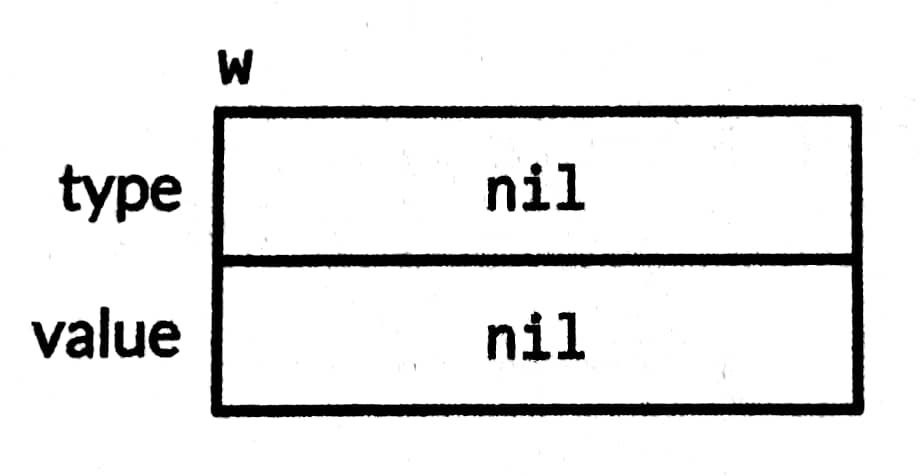
\includegraphics[width=0.4\linewidth]{figures/figura6.1}
\end{center}

Un valore interfaccia è descritto come nil o non-nil a seconda del suo tipo dinamico.

La seconda istruzione assegna un valore di tipo \verb|*os.File| a \verb|w|:
\begin{lstlisting}[frame=single, label={lst:lstlisting6-5.3}]
w = os.Stdout
\end{lstlisting}
Questo assegnamento coinvolge una conversione implicita da un tipo concreto al tipo di interfaccia, ed è equivalente alla conversione esplicita \verb|io.Writer(os.Stdout)|.
Una conversione di questo tipo cattura il tipo e il valore dei suoi operandi.
Il tipo dinamico del valore di interfaccia è impostato al descrittore del tipo per un tipo puntatore \verb|*os.File|, e il suo valore dinamico detiene una copia di \verb|os.Stdout|, che è un puntatore ad una variabile \verb|os.File| rappresentante lo standard output di un processo.
\begin{center}
    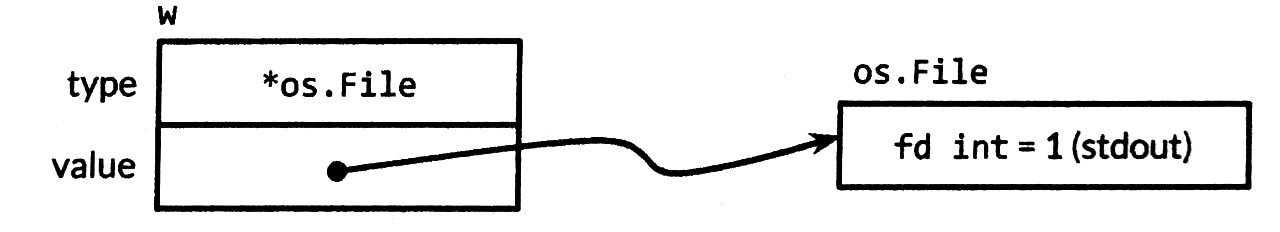
\includegraphics[width=0.5\linewidth]{figures/figura6.2}
\end{center}

In generale, non è possibile conoscere a compile-time quale tipo dinamico del valore di interfaccia sarà, così una chiamata tramite un interfaccia deve usare un \textit{invio dinamico}.
Invece di una chiamata diretta, il compilatore deve generare codice per ottenere l'indirizzo del metodo \verb|Write| dal tipo del descrittore, quindi produrre una chiamata indiretta a quel indirizzo.
L'argomento ricevitore per la chiamata è una copia del valore dinamico dell'interfaccia, \verb|os.Stdout|.
L'effetto è come se si fosse prodotta una chiamata direttamente.

La terza istruzione assegna un valore di tipo \verb|*bytes.Buffer| al valore di interfaccia:
\begin{lstlisting}[frame=single, label={lst:lstlisting6-5.4}]
w = new(bytes.Buffer)
\end{lstlisting}
Il tipo dinamico è ora \verb|*bytes.Buffer| e il valore dinamico è un puntatore al nuovo buffer allocato.
\begin{center}
    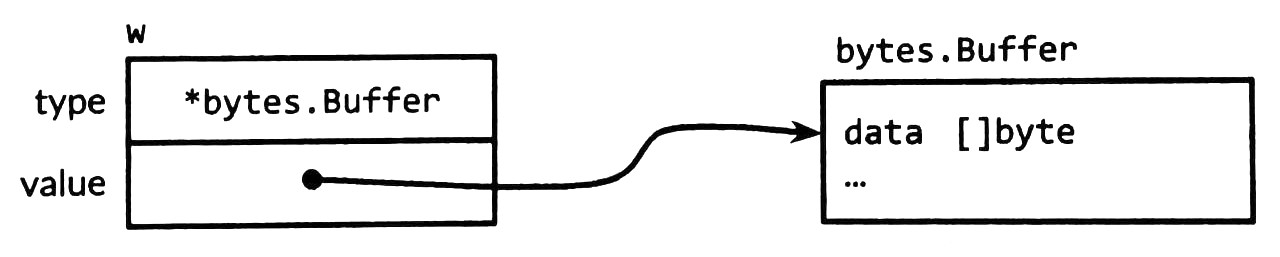
\includegraphics[width=0.5\linewidth]{figures/figura6.3}
\end{center}

Infine, la quarta istruzione assegna \verb|nil| al valore di interfaccia:
\begin{lstlisting}[frame=single, label={lst:lstlisting6-5.5}]
w = nil
\end{lstlisting}
Questo fa il reset di entrambi i suoi componenti a \verb|nil|, ripristinando \verb|w| allo stato della sua dichiarazione.

I valori di interfaccia possono essere confrontati usando \verb|==| e \verb|!=|, quindi utilizzabili anche come chiavi per le map o come gli operandi di un'istruzione switch.
Bisogna comunque fare attenzione, perché se le interfacce hanno stessi tipi dinamici, ma non confrontabili tra loro, allora il confronto fallisce con il lancio di un panic.
\begin{lstlisting}[frame=single, label={lst:lstlisting6-5.6}]
var x interface{} = []int{1, 2, 3}
fmt.Println(x == x) // panic: i tipi []int non sono
                    // confrontabili
\end{lstlisting}
Per questi motivi in generale si possono confrontare i valori di un interfaccia se si è certi che questo contenga valori dinamici di tipi confrontabili.

\section{L'interfaccia error}
\label{sec:interfaccia_error}%
Il tipo predichiarato \verb|error| è un tipo interfaccia con un singolo metodo che restituisce un messaggio d'errore:
\begin{lstlisting}[frame=single, label={lst:lstlisting6-6.1}]
type error interface {
    Error() string
}
\end{lstlisting}
Il modo più semplice per creare un \verb|error| è invocando \verb|errors.New|, che restituisce un nuovo \verb|error| per un dato messaggio d'errore.
L'intero package \verb|errors| è lungo solo 4 righe:
\begin{lstlisting}[frame=single, label={lst:lstlisting6-6.2}]
package errors

func New(text string) error { return &errorString{text} }

type errorString struct { text string }

func (e *errorString) Error() string { return e.text }
\end{lstlisting}
Il sottotipo di \verb|errorString| è una struct, non una stringa, a proteggere una sua rappresentazione da un aggiornamento involontario.
La ragione per cui il puntatore al tipo \verb|*errorString| soddisfa l'interfaccia \verb|error| è perché si vuole che ogni chiamata a \verb|New| allochi un'istanza distinta di \verb|error| diversa da tutte le altre.

Le chiamate a \verb|errors.New| sono relativamente poco frequenti perché esiste una funzione wrapper più conveniente, \verb|fmt.Errorf|, che permette pure la formattazione delle stringhe.




    \chapter{Goroutine e channel}
    \label{ch:goroutine_e_channel}%
    La programmazione concorrente, programma visto come composizione di numerose attività autonome, è l'elemento più importante di questi tempi.
I server web gestiscono richieste per migliaia di client contemporaneamente.
Le app degli smartphone e dei tablet gestiscono le animazioni sull'interfaccia utente mentre simultaneamente eseguono la computazione e le richieste di rete in background.
Anche i tradizionali problemi di batch (lettura dei dati, computazione e scrittura degli output) usano la concorrenza per nascondere la latenza delle operazioni I/O così da sfruttare anche i multiprocessori dei computer moderni, i quali, negli anni, continuano a crescere in numero ma non in velocità.

Go offre due stili di programmazione concorrente.
In questo capitolo vengono esponte le goroutine e i channel, compatibili con la \textit{CSP} o \textit{communicating sequential processes}, un modello di concorrenza dove i valori sono visti come attività indipendenti (goroutine), ma con le variabili confinate alle singole attività.
Nel prossimo capitolo verranno illustrati gli aspetti più tradizionali del modello \textit{shared memory multithreading}.


\section{Goroutine}
\label{sec:goroutine}%
In Go, ogni attività concorrente in esecuzione è detta \textit{goroutine}.
Dato un programma con due funzioni, uno che svolge operazioni di computazione e l'altra che scrive qualche dato in output, si supponga che entrambi non si richiamino a vicenda.
Un programma sequenziale potrebbe chiamare una funzione e solo in seguito l'altra, ma in un programma \textit{concorrente} con due o più goroutine, le chiamate ad \textit{entrambe} le funzioni possono essere svolte contemporaneamente.

Si può pensare per ora alle goroutine come a thread perché la loro differenza è essenzialmente in termini quantitativi e non qualitativi.

Quando un programma viene avviato, la sua unica goroutine è quella che richiama la funzione \verb|main|, definita \textit{main goroutine}.
Le nuove goroutine sono create dall'istruzione \verb|go|.
Sintatticamente, un'istruzione \verb|go| è una funzione ordinaria o una chiamata ad un metodo con la parola chiave \verb|go| come prefisso.
Un'istruzione \verb|go| permette alla funzione di essere chiamata da una nuova e goroutine.
\begin{lstlisting}[frame=single, label={lst:lstlisting7-1.1}]
f()    // chiama f(); attende il risultato
go f() // crea una nuova goroutine che chiama f(); non c'%*\textit{è}*\)
       // attesa
\end{lstlisting}
Nel seguente esempio, la main goroutine computa il 45esimo numero di Fibonacci.
Dato che utilizza un algoritmo inefficiente, essa rimarrà in esecuzione per un tempo considerevole, durante il quale si vorrebbe dire all'utente che il programma è ancora in esecuzione tramite la stampa di uno ``spinner'' testuale.
\begin{lstlisting}[frame=single, label={lst:lstlisting7-1.2}]
func main() {
    go spinner(100 * time.Millisecond)
    const n = 45
    fibN := fib(n) // lento
    fmt.Printf(%*``*\)\rFibonacci(%d) = %d\n%*''*\), n, fibN)
}

func spinner(delay time.Duration) {
    for {
        for _, r := range `-\|/' {
            fmt.Printf(%*``*\)\r%c%*''*\), r)
            time.Sleep(delay)
        }
    }
}
\end{lstlisting}
\begin{lstlisting}[frame=single, label={lst:lstlisting7-1.3}]
func fib(x int) int {
    if x < 2 {
        return x
    }
    return fib(x-1) + fib(x-2)
}
\end{lstlisting}
Una volta computato il risultato, la funzione \verb|main| lo stampa e quindi effettua il return.
Quando questo succede, tutte le goroutine vengono bruscamente terminate e il programma si chiude.
Non esistono altri modi per terminare una goroutine se non chiudere il programma o effettuare il return della funzione \verb|main|, questo perché una goroutine non può terminarne un'altra;
esistono tuttavia possibilità di metterle in comunicazione.


\section{Esempio: clock server concorrente}
\label{sec:esempio_clock_server_concorrente}
%
La rete è un dominio naturale dove usare la concorrenza perché vengono tipicamente gestite molte connessioni provenienti da diversi client allo stesso tempo, consci che ogni client è in genere indipendente da tutti gli altri.

Esponiamo come primo esempio un clock server sequenziale che scrive l'orario corrente al client ad ogni secondo:
\begin{lstlisting}[frame=single, label={lst:lstlisting7-2.1}]
// Clock1 %*\textit{è}*\) un server TCP che periodicamente scrive l'orario.
func main() {
    listener, err := net.Listen(%*``*\)tcp%*''*\), %*``*\)localhost:8000%*''*\))
    if err != nil {
        log.Fatal(err)
    }
    for {
        conn, err := listener.Accept()
        if err != nil {
            log.Print(err) // p.e., connessione fallita
            continue
        }
        handleConn(conn) // gestisce una connessione alla volta
    }
}

func handleConn(c net.Conn) {
    defer c.Close()
    for {
        _, err := io.WriteString(c,
            time.Now().Format(%*``*\)15:04:05\n%*''*\)))
        if err != nil {
            return // p.e., client disconnesso
        }
        time.Sleep(1 * time.Second)
    }
}
\end{lstlisting}
La funzione \verb|Listen| crea un \verb|net.Listener|, un oggetto che ``ascolta'' l'arrivo di connessioni in ingresso sullo porta di rete designata, in questo caso la porta TCP \verb|localhost:8000|.
Il metodo \verb|Accept| del listener blocca il listener stesso in attesa di una richiesta di connessione, quindi restituisce un oggetto \verb|net.Conn| rappresentante la connessione attesa.

La funzione \verb|handleConn| gestisce una completa connessione del client.
In un ciclo, essa scrive l'orario corrente, \verb|time.Now()|, al client.
Finché \verb|net.Conn| soddisfa l'interfaccia \verb|io.Writer|, si può scrivere direttamente al client.
Il ciclo finisce quando la scrittura fallisce, che molto probabilmente accade quando il client si disconnette, momento in cui \verb|handleConn| chiude il proprio lato della connessione usando la chiama differita a \verb|Close| e torna ad attendere la richiesta di una connessione.

Sul lato client il programma è il seguente:
\begin{lstlisting}[frame=single, label={lst:lstlisting7-2.2}]
// Netcat1 %*\textit{è}*\) un client TCP di sola lettura
func main() {
    conn, err := net.Dial(%*``*\)tcp%*''*\), %*``*\)localhost:8000%*''*\))
    if err != nil {
        log.Fatal(err)
    }
    defer conn.Close()
    mustCopy(os.Stdout, conn)
}

func mustCopy(dst io.Writer, src io.Reader) {
    if _, err := io.Copy(dst, src); err != nil {
        log.Fatal(err)
    }
}
\end{lstlisting}
Questo programma legge i dati dalla connessione e li scrive sullo standard output fino a quando non viene incontrato una condizione di end-of-file o un errore.
Eseguendo due client allo stesso tempo si esegue il seguente risultato:
\begin{lstlisting}[language=bash, frame=L, label={lst:lstlisting7-2.3}]
$ ./netcat1
13:56:34
13:56:35        $ ./netcat1
13:56:36
^C
                13:56:38
                13:56:39
                13:56:40
                ^C
\end{lstlisting}
In questa implementazione il secondo client è obbligato ad aspettare che il primo client finisca perché il server è \textit{sequenziale};
il server si occupa di un client alla volta.
Per rendere il server concorrente serve solo una piccola modifica: l'aggiunta della parola chiave \verb|go| alla chiamata di \verb|handleConn| fa sì che ogni chiamata venga eseguita nella propria goroutine.
\begin{lstlisting}[frame=single, label={lst:lstlisting7-2.4}]
func main() {
    listener, err := net.Listen(%*``*\)tcp%*''*\), %*``*\)localhost:8000%*''*\))
    if err != nil {
        log.Fatal(err)
    }
    for {
        conn, err := listener.Accept()
        if err != nil {
            log.Print(err) // p.e., connessione fallita
            continue
        }
        go handleConn(conn) // gestisce le connessioni in modo
                            // concorrente
    }
}
\end{lstlisting}
Ora più client possono ricevere l'orario contemporaneamente:
\begin{lstlisting}[language=bash, frame=L, label={lst:lstlisting7-2.5}]
$ ./netcat2
13:58:54
13:58:55        $ ./netcat2
13:58:56        13:58:56
13:58:57        13:58:57
13:58:58        13:58:58
13:58:59        ^C
13:59:00
13:59:01        $ ./netcat2
13:59:02        13:59:02
13:59:03        13:59:03
^C              13:59:04
                ^C
\end{lstlisting}

\section{I channel}
\label{sec:channel}
%
Se in Go le goroutine sono le attività di un programma concorrente, i channel sono le connessioni fra di loro.
Un channel è un meccanismo di comunicazione che permette di inviare valori ad un'altra goroutine.
Ogni channel è un condotto per i valori di un tipo particolare, detto \textit{tipo elementare} del channel.
Il tipo del channel che ha elementi di tipo \verb|int| è indicato come \verb|chan int|.

Per creare un channel viene usata la funzione built-in \verb|make|:
\begin{lstlisting}[frame=single, label={lst:lstlisting7-4.1}]
ch := make(chan int) // ch ha tipo `chan int'
\end{lstlisting}
Come per le map, un channel è un \textit{riferimento} ad una struttura dati creata da \verb|make|.
Quando si fa una copia ad un channel o quando viene passato come argomento ad una funzione, in realtà se ne sta copiando il riferimento, così il chiamante e il chiamato si riferiranno alla stessa struttura dati.
Come per gli altri tipi referenziati, il valore zero di un channel è il \verb|nil|.

Due channel dello stesso tipo possono essere confrontati con \verb|==|.
Il confronto è vero se entrambi sono riferimenti alla stessa struttura dati channel.
Un channel può anche essere confrontato con un \verb|nil|.

Un channel ha due operazioni principali, \textit{send} e \textit{receive}, conosciuti insieme come operazioni di \textit{communication}.
Un operazione di send trasmette, per mezzo del channel, un valore da una goroutine ad un altra goroutine che esegue una corrispondente operazione di receive.
Entrambe le operazioni sono scritte usando l'operatore \verb|<-|.
In un'operazione di send, \verb|<-| separa il channel dall'operando valore.
In un'operazione di receive \verb|<-| precede l'operando channel.
Un'operazione di receive il cui risultato non viene utilizzato è un'istruzione valida.
\begin{lstlisting}[frame=single, label={lst:lstlisting7-4.2}]
ch <- x // un'istruzione di send

x = <-ch // un'espressione di receive in un'operazione di
         // assegnamento
<-ch     // un'istruzione di receive; il risultato %*\textit{è}*\) scartato
\end{lstlisting}
I channel supportano una terza operazione, \textit{close}, che imposta un flag sul channel ad indicare che nessun valore verrà più inviato tramite esso;
tentare comunque un invio causa un panic.
Le operazioni di receive su un channel chiuso restituiscono i valori che sono stati inviati prima della chiusura fino a quando non finiscono;
qualunque successiva operazione di receive viene risolta immediatamente producendo il valore zero del tipo elementare del channel.

Per chiudere un channel, bisogna chiamare la funzione built-in \verb|close|:
\begin{lstlisting}[frame=single, label={lst:lstlisting7-4.3}]
close(ch)
\end{lstlisting}
Un channel creato con una chiamata a \verb|make| viene detto un \textit{unbuffered} channel, ma \verb|make| accetta un secondo argomento opzionale, un intero detto \textit{capacity} del channel.
Se la capacity del channel è diversa da zero, \verb|make| crea un \textit{buffered} channel.
\begin{lstlisting}[frame=single, label={lst:lstlisting7-4.4}]
ch = make(chan int)    // unbuffered channel
ch = make(chan int, 0) // unbuffered channel
ch = make(chan int, 3) // buffered channel con capacity 3
\end{lstlisting}

\subsection{Unbuffered channel}
\label{subsec:unbuffered_channel}%
Un'operazione di send su un unbuffered channel blocca la goroutine mittente fino a quando un'altra goroutine esegue una corrispondente operazione di receive sullo stesso channel, momento in cui il valore è trasmesso e entrambe le goroutine possono proseguire la loro esecuzione.
Al contrario, se l'operazione di receive viene eseguita prima, la goroutine destinataria viene bloccata fino a quando un'altra goroutine eseguirà una send sullo stesso channel.

La comunicazione su un unbuffered channel costringe le goroutine, mittente e destinatario, a \textit{sincronizzarsi}.
Per questa ragione, gli unbuffered channel sono qualche volta detti channel \textit{sincronizzati}.
Quando un valore è inviato su un unbuffered channel, la ricezione del valore \textit{avviene prima} del risveglio della goroutine mittente.

Quando \textit{x} non viene eseguito nè prima di \textit{y} nè dopo \textit{y}, si dice che \textit{x è concorrente ad y}.
Questo non vuol dire necessariamente che \textit{x} e \textit{y} sono simultanei, piuttosto che non è possibile fare ipotesi sul loro ordine d'esecuzione.

Per far sì che la main goroutine attenda la fine della goroutine in background prima di chiudere il programma, si può usare un channel per sincronizzare le due goroutine:
\begin{lstlisting}[frame=single, label={lst:lstlisting7-4-1.1}]
func main() {
   conn, err := net.Dial(%*``*\)tcp%*''*\), %*``*\)localhost:8000%*''*\))
   if err != nil {
      log.Fatal(err)
   }
   done := make(chan struct{})
   go func() {
      io.Copy(os.Stdout, conn) // NOTA: gli errori sono ignorati
      log.Println(%*``*\)done%*''*\))
      done <- struct{}{} // si avvisa la main goroutine
   }()
   mustCopy(conn, os.Stdin)
   conn.Close()
   <-done // attende la fine della goroutine in background
}

func mustCopy(dst io.Writer, src io.Reader) {
   if _, err := io.Copy(dst, src); err != nil {
      log.Fatal(err)
   }
}
\end{lstlisting}
Quando l'utente chiude lo stream di standard input, \verb|mustCopy| si conclude e la main goroutine chiama \verb|conn.Close()|, chiudendo entrambe le parti della connesione alla rete.
La chiusura del lato scrittura della connessione permette al server di vedere una condizione di end-of-file.
La chiusura del lato lettura della connessione causa alla chiamata di \verb|io.Copy| sulla goroutine in background di restituire un errore ``read from closed connection'' (lettura da una connessione chiusa).

Prima di restituire il risultato, la goroutine in background registra un messaggio, quindi invia un valore sul channel \verb|done|.
La main goroutine attende di ricevere questo valore prima di restituire anche lei il risultato.
Come risultato il programma registra sempre il messaggio ``\verb|done|'' prima di terminare sul lato client.

I messaggi inviati sui channel hanno due aspetti importanti.
Ogni messaggio ha un valore, ma qualche volta sono importanti anche la comunicazione in sè e il momento in cui questa avviene.
I messaggi sono definiti \textit{eventi} quando si desidera porre accento su quest'aspetto.
Quando l'evento non porta informazioni aggiuntive allora il suo unico obiettivo è la sincronizzazione, e in questo caso viene usato come tipo elementare del channel il tipo \verb|struct{}|, anche se è comune usare un channel di \verb|bool| o \verb|int| per lo stesso obiettivo fintanto che \verb|done <- 1| è più immediato di \verb|done <- struct{}{}|.

\subsection{Pipeline}
\label{subsec:pipeline}%
I channel possono essere usati per connettere le goroutine insieme cosicché l'output di uno è l'input dell'altro.
Questi è detto \textit{pipeline}.
Il seguente programma consiste di tre goroutine connesse da due channel, come mostrato schematicamente in figura.
\begin{center}
    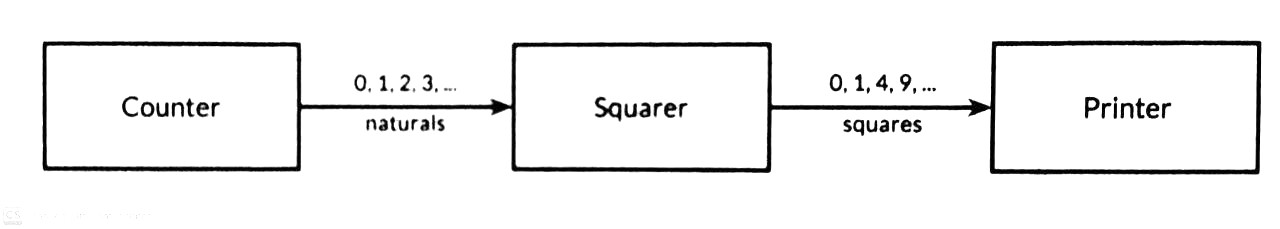
\includegraphics[width=0.8\linewidth]{figures/figure7.1}
\end{center}
La prima goroutine, \textit{counter}, genera gli interi 0, 1, 2, \ldots, e li invia su un channel alla seconda goroutine, \textit{squarer}, che riceve ogni valore, lo eleva al quadrato, e invia il risultato su un altro channel alla terza goroutine, \textit{printer}, che riceve i valori e li stampa.
Per chiarezza di quest'esempio, si è intenzionalmente scelto una funzione davvero semplice per spiegare il funzionamento della pipeline.
\begin{lstlisting}[frame=single, label={lst:lstlisting7-4-2.1}]
func main() {
    naturals := make(chan int)
    squares := make(chan int)

    // Counter
    go func() {
        for x := 0; ; x++ {
            naturals <- x
        }
    }()

    // Squarer
    go func() {
        for {
            x := <-naturals
            squares <- x * x
        }
    }()

    // Printer (nella main goroutine)
    for {
        fmt.Println(<-squares)
    }
}
\end{lstlisting}
Se il mittente conosce che non ci sono più valori da inviare sul channel, è bene comunicarlo alla goroutine destinataria così da non farlo attendere.
Questo è realizzato con la \textit{chiusura} del channel con la funzione built-in \verb|close|:
\begin{lstlisting}[frame=single, label={lst:lstlisting7-4-2.2}]
close(naturals)
\end{lstlisting}
Dopo che un channel è stato chiuso, qualunque altra operazione di send restituirà un panic.
Dopo che il channel chiuso sia stato \textit{svuotato}, ovvero dopo che l'ultimo elemento inviato sia stato recepito, tutte le successive operazioni di receive verranno risolte restituendo un valore zero per il tipo elementare del channel.
Chiudendo il channel \verb|naturals| si causerà al ciclo di squarer di ricevere uno stream senza fine di valori zero, e di inviare tali valori al printer.

Non esiste un modo diretto per capire se un channel è stato chiuso, ma esiste una variante dell'operazione di receive che produce due risultati: l'elemento ricevuto dal channel più un valore booleano, denominato per convenzione \verb|ok|, che è \verb|true| nel caso di un'operazione di receive completata con successo e \verb|false| nel caso di un'operazione di receive su un channel chiuso e svuotato.
Usando questa funzionalità, il ciclo di squarer può essere modificato così da interromperlo quando il channel \verb|naturals| è svuotato e chiudere a cascata il channel \verb|squares|.
\begin{lstlisting}[frame=single, label={lst:lstlisting7-4-2.3}]
go func() {
    for {
        x, ok := <-naturals
        if !ok {
            break // il channel %*\textit{è}*\) stato chiuso e svuotato
        }
        squares <- x * x
    }
    close(squares)
}()
\end{lstlisting}
Il linguaggio permette di usare un ciclo \verb|range| per iterare anche su un channel.
Questo è sintatticamente più conveniente per ricevere tutti i valori inviati su un channel e terminare il ciclo dopo l'ultimo.
\begin{lstlisting}[frame=single, label={lst:lstlisting7-4-2.4}]
func main() {
    naturals := make(chan int)
    squares := make(chan int)

    // Counter
    go func() {
        for x := 0; x < 100; x++ {
            naturals <- x
        }
        close(naturals)
    }()

    // Squarer
    go func() {
        for x := range naturals {
            squares <- x * x
        }
        close(squares)
    }()

    // Printer (nella main goroutine)
    for x := range squares {
        fmt.Println(x)
    }
}
\end{lstlisting}
Non è sempre necessario chiudere un channel, lo è nel momento in cui è importante avvisare la goroutine destinaria che tutti i valori sono stati inviati, altrimenti può anche essere tralasciato perché il garbage collector si occuperà di determinare quando un channel è diventato irraggiungibile e quindi riciclarlo anche se non chiuso.
(Questo discorso non vale per i file;
i file devono sempre essere chiusi tramite chiamata al metodo \verb|Close|).

\subsection{Tipi di channel unidirezionali}
\label{subsec:tipi_di_channel_unidirezionali}%
Non appena un programma cresce, è naturale spezzare grandi funzioni in pezzi più piccoli.
La funzione \verb|main| proposta alle pagine precedenti può essere suddivisa in tre funzioni:
\begin{lstlisting}[frame=single, label={lst:lstlisting7-4-3.1}]
func counter(out chan int)
func squarer(out, in chan int)
func printer(in chan int)
\end{lstlisting}
La funzione \verb|squarer|, posto in mezzo alla pipeline, riceve due parametri, il channel di input e il channel di output.
Entrambi hanno lo stesso tipo, ma i loro usi opposti: \verb|in| è solo per ricevere, mentre \verb|out| solo per inviare.
I nomi \verb|in| e \verb|out| rafforzano questa idea, ma nulla vieta a \verb|squarer| di inviare su \verb|in| e di ricevere da \verb|out|.

Quando un channel è passato come parametro di una funzione, è quasi sempre dato con l'intento di usarlo esclusivamente per inviare o esclusivamente per ricevere.

Per documentare questo intento e prevenire un uso scorretto, il type system di Go offre i tipi di channel \textit{unidirezionali} per permettere solo una fra le operazioni di send e receive.
Il tipo \verb|chan<- int|, un channel di \textit{solo invio} di \verb|int|, permette solo gli invii.
Al contrario, il tipo \verb|<-chan int|, un channel di \textit{sola ricezione} di \verb|int|, permette solo le ricezioni.
Violazioni di questi usi sono individuati a compile time.

Dato che l'operazione di \verb|close| asserisce che nessuna operazione di send verrà più effettuata su un channel, allora solo la goroutine mittente potrà chiamarla, e per questa ragione è un errore a compile time provare a chiudere un channel di sola ricezione.
\begin{lstlisting}[frame=single, label={lst:lstlisting7-4-3.2}]
func counter(out chan<- int) {
    for x := 0; x < 100; x++ {
        out <- x
    }
    close(out)
}

func squarer(out chan<- int, int <-chan int) {
    for v := range in {
        out <- v * v
    }
    close(out)
}

func printer(in <-chan int) {
    for v := range in {
        fmt.Println(v)
    }
}
\end{lstlisting}
\begin{lstlisting}[frame=single, label={lst:lstlisting7-4-3.3}]
func main() {
    naturals := make(chan int)
    squares := make(chan int)

    go counter(naturals)
    go squarer(squares, naturals)
    printer(squares)
}
\end{lstlisting}
La chiamata \verb|counter(naturals)| converte \verb|naturals| dal tipo \verb|chan int| al tipo \verb|chan<- int| in modo implicito.
La chiamata a \verb|printer(squares)| esegue implicitamente una conversione simile a \verb|<-chan int|.
Le conversioni dei tipi di channel da bidirezionali a unidirezionali sono permesse in ogni assegnazione.
Non esiste però modo di tornare indietro: un channel convertito in unidirezionale non può più tornare ad essere bidirezionale.

\subsection{Buffered channel}
\label{subsec:buffered_channel}%
Un buffered channel ha una coda di elementi.
La dimensione massima della coda è decisa quando viene creato il channel, dall'argomento capacity in \verb|make|.
La seguente istruzione crea un buffered channel in grado di ospitare al più tre valori \verb|string|.
La figura mostra anche una rappresentazione di \verb|ch| e del channel a cui si riferisce.
\begin{lstlisting}[frame=single, label={lst:lstlisting7-4-4.1}]
ch = make(chan string, 3)
\end{lstlisting}
\begin{center}
    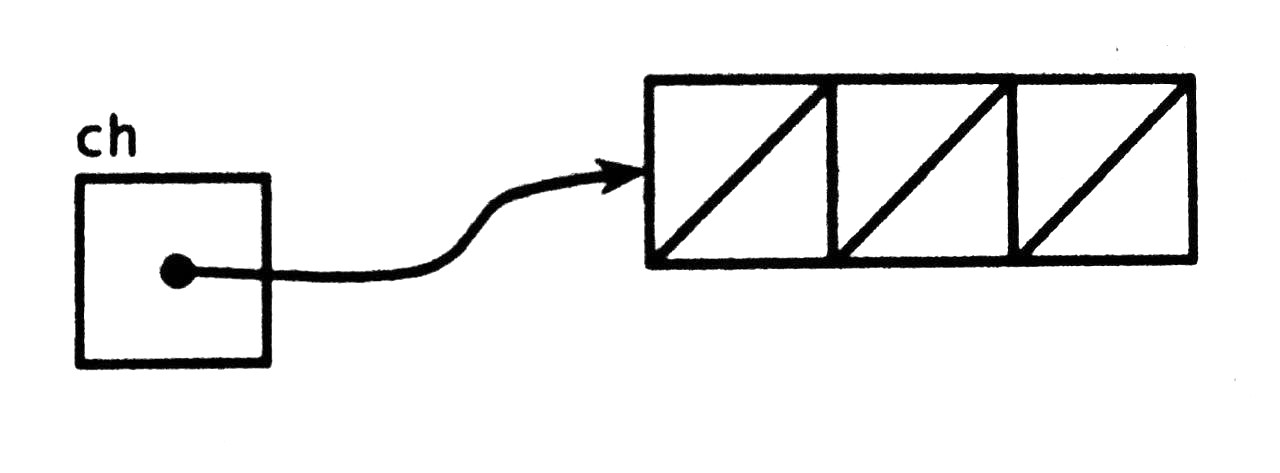
\includegraphics[width=0.5\linewidth]{figures/figure7.2}
\end{center}
Un'operazione di send su un buffered channel inserisce un elemento in coda alla fila d'attesa , e l'operazione di receive rimove un elemento dalla testa della fila.
Se il channel è pieno, l'operazione di send blocca la propria goroutine fino a quando non viene fatto spazio in seguito all'operazione di receive di un'altra goroutine.
Al contrario, se il channel è vuoto, un'operazione di receive blocca la propria goroutine fino a quando un'altra goroutine non esegue un'operazione di send sullo stesso channel.
\begin{lstlisting}[frame=single, label={lst:lstlisting7-4-4.2}]
ch <- %*``*\)A%*''*\)
ch <- %*``*\)B%*''*\)
ch <- %*``*\)C%*''*\)
\end{lstlisting}
Dopo aver eseguito queste tre istruzioni, il channel è pieno e una quarta operazione di send verrà bloccata.
\begin{center}
    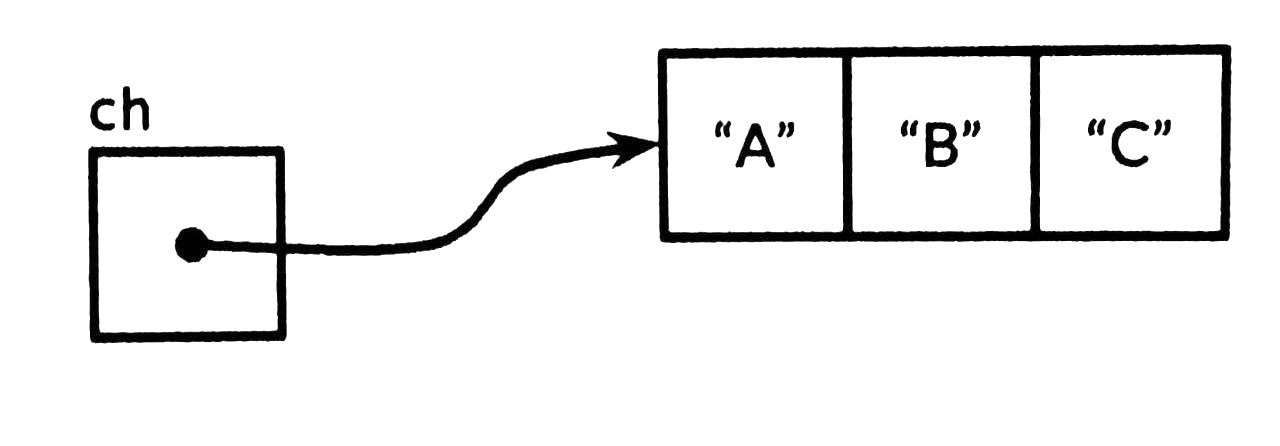
\includegraphics[width=0.5\linewidth]{figures/figure7.3}
\end{center}
Se si riceve un valore,
\begin{lstlisting}[frame=single, label={lst:lstlisting7-4-4.3}]
fmt.Println(<-ch)
\end{lstlisting}
Output:
\begin{lstlisting}[language=bash, frame=L, label={lst:lstlisting7-4-4.4}]
A
\end{lstlisting}
il channel non sarà più nè pieno nè vuoto, quindi sia un'operazione di send che una di receive potranno procedere senza essere bloccati.
In questo modo, il buffer del channel separa le goroutine mittenti e destinatari.
\begin{center}
    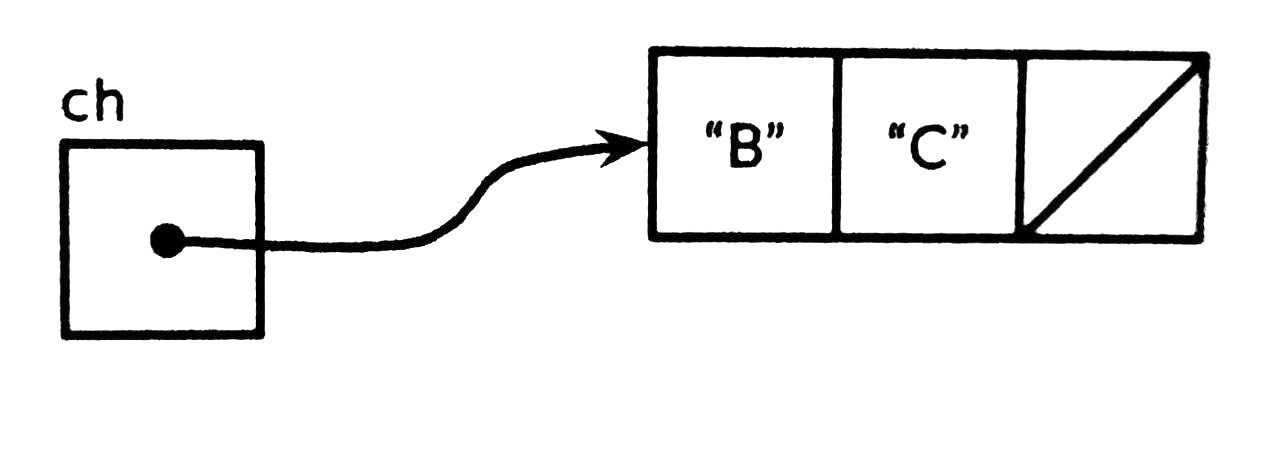
\includegraphics[width=0.5\linewidth]{figures/figure7.4}
\end{center}
Nel caso un programma voglia conoscere la capacità del buffer del channel può richiamare la funzione \verb|cap|:
\begin{lstlisting}[frame=single, label={lst:lstlisting7-4-4.5}]
fmt.Println(cap(ch))
\end{lstlisting}
Output:
\begin{lstlisting}[language=bash, frame=L, label={lst:lstlisting7-4-4.6}]
3
\end{lstlisting}
Quando applicato al channel, la funzione \verb|len| restituisce il numero di elementi al momento presenti nel buffer.

Il seguente esempio presenta un'applicazione di un buffered channel.
Tale programma fa richieste in parallelo a tre \textit{mirror}, ovvero server equivalenti ma geograficamente distribuiti.
Essi inviano la loro risposta su un buffered channel, quindi ricevono e restituiscono solo la prima risposta, che è la più veloce ad arrivare.
Quindi \verb|mirrorQuery| restituisce un risultato anche prima della risposta dei due server più lenti.
\begin{lstlisting}[frame=single, label={lst:lstlisting7-4-4.7}]
func mirrorQuery() string {
responses := make(chan string, 3)
    go func() { responses <- request(%*``*\)asia.gopl.io%*''*\)) }()
    go func() { responses <- request(%*``*\)europe.gopl.io%*''*\)) }()
    go func() { responses <- request(%*``*\)americas.gopl.io%*''*\)) }()
    return <-responses // Ritorna la risposta pi%*\textit{ù}*\) veloce
}

func request(hostname string) (response string) { /* ... */ }
\end{lstlisting}
La scelta fra un unbuffered e buffered channel e la scelta della capacity per il buffered channel possono entrambe influenzare la correttezza del programma.
Gli unbuffered channel offrono una forte garanzia di sincronizzazione perché ogni operazione di send è sincronizzata con la corrispettiva operazione di receive;
con i buffered channel, queste operazioni sono slegate.
Inoltre, quando si conosce la dimensione massima del numero di valori che possono essere inviati su un channel, è utile creare un buffered channel di quella dimensione ed effettuare tutti i send ancor prima che il primo valore sia ricevuto dal destinatario.
Un fallimento nell'allocazione di un buffer di sufficiente capacity potrebbe portare il programma ad un deadlock.

\section{Esempio: Chat Server}
\label{sec:esempio_chat_server}
%
Un chat server permette a molti utenti di inviarsi l'un l'altro messaggi testuali.
Ci sono quattro tipologie di goroutine in questo programma.
C'è un'istanza a testa per la goroutine \verb|main| e \verb|broadcast|, e per ogni connessione client c'è una goroutine \verb|handleConn| e una \verb|clientWriter|.

Il compito della main goroutine è rimanere in ascolto e di accettare connessioni di rete in input da parte di client.
Per ognuno di essi, il main crea una nuova goroutine \verb|handleConn|.
\begin{lstlisting}[frame=single, label={lst:lstlisting7-10.1}]
func main() {
    listener, err := net.Listen(%*``*\)tcp%*''*\), %*``*\)localhost:8000%*''*\))
    if err != nil {
        log.Fatal(err)
    }

    go broadcaster()
    for {
        conn, err := listener.Accept()
        if err != nil {
            log.Print(err)
            continue
        }
        go handleConn(conn)
    }
}
\end{lstlisting}
Il broadcaster ha una variabile locale \verb|clients| che tiene registrato l'insieme di tutti i client correntemente connessi.
Per ogni client viene memorizzata solo l'identità del loro channel di messaggi in uscita.
\begin{lstlisting}[frame=single, label={lst:lstlisting7-10.2}]
type client chan<- string // un channel di messaggi in uscita

var (
    entering = make(chan client)
    leaving  = make(chan client)
    messages = make(chan string) // tutti i messaggi client in
                                 // arrivo
)

func broadcaster() {
    clients := make(map[client]bool) // tutti i client connessi
    for {
        select {
        case msg := <-messages:
            // Trasmette il messaggio in entrata ai
            // channel dei messaggi in uscita di tutti i client.
            for cli := range clients {
                cli <- msg
            }
        case cli := <-entering:
            clients[cli] = true
        case cli := <-leaving:
            delete(clients, cli)
            close(cli)
        }
    }
}
\end{lstlisting}
Il broadcaster rimane in ascolto sui channel globali \verb|entering| e \verb|leaving| per annunci sull'arrivo o sulla partenza di client.
Quando riceve un annuncio di questi eventi, aggiorna l'insieme \verb|clients|, e se l'evento è di partenza, chiude il channel di messaggi in uscita del client corrispondente.
Il broadcaster rimane anche in ascolto di eventi sul channel globale \verb|messages|, dove ogni client invia tutti i suoi messaggi in arrivo.
Quando il broadcaster riceve uno di questi eventi, invia a tutti i client connessi il messaggio.

Ora si veda la goroutine dedicata al client sul server.
La funzione \verb|handleConn| crea un channel di messaggi in uscita per il proprio client e annuncia l'arrivo dello stesso client al broadcaster sul channel \verb|entering|.
A questo punto legge ogni linea di testo dal client, invia ogni linea al broadcaster sul channel di messaggi in arrivo, aggiungendo come prefisso ad ogni messaggio l'identità del mittente.
Una volta che non c'è più nulla da leggere dal client, \verb|handleConn| annuncia la partenza del client sul channel \verb|leaving| e chiude la connessione.
\begin{lstlisting}[frame=single, label={lst:lstlisting7-10.3}]
func handleConn(conn net.Conn) {
    ch := make(chan string) // messaggi client in uscita
    go clientWriter(conn, ch)

    who := conn.RemoteAddr().String()
    ch <- %*``*\)You are %*''*\) + who
    messages <- who + %*``*\) has arrived%*''*\)
    entering <- ch

    input := bufio.NewScanner(conn)
    for input.Scan() {
        messages <- who + %*``*\): %*''*\) + input.Text()
    }
    // NOTA: si ignorano potenziali errori di input.Err()

    leaving <- ch
    messages <- who + %*``*\) has left%*''*\)
    conn.Close()
}

func clientWriter(conn net.Conn, ch <-chan string) {
    for msg := range ch {
        fmt.Fprintln(conn, msg) // NOTA: si ignorano gli errori
                                // di rete
    }
}
\end{lstlisting}
In aggiunta, \verb|handleConn| crea una goroutine \verb|clientWriter| per ogni client che riceve un messaggio in broadcast sul channel di messaggi in uscita del client e li scrive sulla connessione di rete del client.
Il ciclo del writer del client termina quando il broadcaster chiude il channel dopo aver ricevuto la notifica di \verb|leaving|.

Per il lato client invece viene utilizzato il programma esposto nel paragrafo \textbf{Unbuffered channel} di questo capitolo.
Una simulazione da linea di comando:
\begin{lstlisting}[language=bash, frame=L, label={lst:lstlisting7-10.4}]
$ go build chat
$ go build netcat3
$ ./chat &
$ ./netcat3
You are 127.0.0.1:64208         $ ./netcat3
127.0.0.1:64211 has arrived     You are 127.0.0.1:64211
Hi!
127.0.0.1:64208: Hi!            127.0.0.1:64208: Hi!
                                Hi yourself.
127.0.0.1:64211 Hi yourself.    127.0.0.1:64211: Hi yourself.
^C
                                127.0.0.1:64208 has left
$ ./netcat3
You are 127.0.0.1:64216         127.0.0.1:64216 has arrived
                                Welcome.
127.0.0.1:64211: Welcome.       127.0.0.1:64211: Welcome.
                                ^C
127.0.0.1:64211 has left
\end{lstlisting}
Mentre il server ospita una sessione di chat per $n$ client, il programma esegue $2n+2$ goroutine comunicanti in modo concorrente, anche se necessita di un'esplicita operazione di lock.
La \verb|clients| map è confinata in una singola goroutine, nel broadcaster, così non può essere acceduta in modo concorrente.
Le uniche variabili condivise fra più goroutine sono i channel e le istanze di \verb|net.Conn|, i quali sono entrambi \textit{concurrency safe}.




    \chapter{Concorrenza con variabili condivise}
    \label{ch:concorrenza_con_variabili_condivise}%
    In questo capitolo si pone maggiormente l'attenzione sui meccanismi della concorrenza.
In particolare, si affrontano i problemi legati alla condivisione di variabili fra molteplici goroutine, le tecniche analitiche per riconoscere questi problemi e i pattern per risolverli.
Infine verrà esposta la differenza fra goroutine e thread del sistema operativo.


\section{Race condition}
\label{sec:race_condition}
%
In un programma sequenziale, ovvero un programma con un'unica goroutine, gli step di un programma vengono eseguiti in un ordine familiare determinato dalla logica del programma.
Per esempio, in una sequenza di istruzioni, il primo viene eseguito prima del secondo, e così via.
In un programma con due o più goroutine, gli step che una goroutine deve eseguire vengono sempre eseguiti in un ordine familiare, ma in generale non è possibile sapere se un evento $x$ in una goroutine accade prima di un evento $y$ in un'altra goroutine, o se accade dopo, o se simultaneamente.
Quando non si conosce l'ordine di esecuzione di due eventi, essi sono detti \textit{concorrenti}.

Considerando una funzione che lavora correttamente in un programma sequenziale, tale funzione è \textit{concurrency-safe} se continua a lavorare correttamente anche se chiamata in modo concorrente.
Si può generalizzare questa definizione ad un insieme di funzioni che si richiamano, come i metodi e le operazioni di un tipo particolare.
Un tipo è concurrency-safe se tutti i suoi metodi e operazioni accessibili sono concurrency-safe.

Si può produrre un programma concurrency-safe senza rendere ogni tipo concreto tale.
Infatti, i tipi concurrency-safe sono l'eccezione piuttosto che la regola, per cui bisogna accedere ad una variabile concorrente solo se la documentazione di quel tipo dice che è sicuro.
Gli accessi concorrenti a molte variabili sono evitate sia \textit{confinandole} in goroutine singole che mantenendo un alto livello di invarianza di \textit{mutua esclusione}.

In contrasto, le funzioni esportate a livello di package ci si aspetta \textit{siano} in generale concurrency-safe.
Fintanto che le variabili a livello di package non sono confinate in una singola goroutine, le funzioni che le modificano devono assicurare la mutua esclusione.

Ci sono molte ragioni per cui una funzione non debba lavorare quando chiamata in modo concorrente, inclusi i deadlock, livelock e la starvation delle risorse.
In questo capitolo verrà solo affrontata la \textit{race condition}.

Una race condition è una situazione in cui il programma non restituisce il corretto risultato per qualche operazione di più goroutine.
Le race condition sono perniciose perché possono rimanere latenti in un programma e apparire poco frequentemente, se non sotto un grosso carico di lavoro o quando usate in certe piattaforme o architetture.
Questo le rende difficili da riprodurre e da diagnosticare.

Prendiamo un tipico esempio per chiarire la serietà del problema:
\begin{lstlisting}[frame=single, label={lst:lstlisting9-1.1}]
var balance int

func Deposit(amount int) { balance = balance + amount }

func Balance() int { return balance }
\end{lstlisting}
Se in questo programma si richiamano le funzioni in modo concorrente, \verb|Balance| non è più garantito essere corretto.
Si considerino le seguenti goroutine:
\begin{lstlisting}[frame=single, label={lst:lstlisting9-1.2}]
// Alice:
go func() {
    bank.Deposit(200)               // A1
    fmt.Println(%*``*\)=%*''*\), bank.Balance()) // A2
}()

// Bob:
go bank.Deposit(100) // B
\end{lstlisting}
Alice deposita \dollar 200, quindi controlla il suo bilancio, mentre Bob deposita \dollar 100.
Fintanto che le istruzioni \verb|A1| e \verb|A2| vengono eseguite in modo concorrente con \verb|B|, si può cadere in errore pensando di avere solo tre scenari (A1+A2+B, A1+B+A2, B+A1+A2).
Il problema è che B può accadere simultaneamente ad A1, e quindi avere un risultato di questo tipo:
\begin{lstlisting}[label={lst:lstlisting9-1.3}]
Data	race
        0
A1r     0       ... = balance + amount
B       100
A1w     200     balance = ...
A2      %*``*\)= 200%*''*\)
\end{lstlisting}
Dopo \verb|A1r|, l'espressione \verb|balance + amount| vale $200$, così questo sarà il valore scritto durante \verb|A1w|, anche se nel frattempo viene eseguito un'altro deposito.
Il bilancio finale è di soli \dollar 200.

Questo programma contiene la race condition detta \textit{data race}.
Un data race accade ogni volta che due goroutine accedono alla stessa variabile in modo concorrente e almeno uno dei due accessi sia una scrittura.

Questo problema diventa ancor più vulnerabile e quindi evidente se i data race coinvolgono una variabile di un tipo più grande, come un'interfaccia, una stringa o una slice.

Il primo modo per evitare una race condition è non fare scritture.
Si consideri la seguente map, popolata in modo pigro in quanto ogni chiave è richiesta per la prima volta.
Se \verb|Icon| è invocato in modo sequenziale, il programma lavora bene, ma se \verb|Icon| è invocato in modo concorrente, allora c'è un data race per l'accesso alla map.
\begin{lstlisting}[frame=single, label={lst:lstlisting9-1.4}]
var icons = make(map[string]image.Image)

func loadIcon(name string) image.Image

// NOTA: non %*\textit{è}*\) concurrency-safe
func Icon(name string) image.Image {
    icon, ok := icons[name]
    if !ok {
        icon = loadIcon(name)
        icons[name] = icon
    }
    return icon
}
\end{lstlisting}
Se invece venisse inizializzata la map con tutte le entry necessarie prima di creare la seconda goroutine e non la si modificasse mai più, allora si avrebbe la concurrency-safe perché non ci sarebbero scritture.
\begin{lstlisting}[frame=single, label={lst:lstlisting9-1.5}]
var icons = map[string]image.Image {
    %*``*\)spades.png%*''*\):   loadIcon(%*``*\)spades.png%*''*\)),
    %*``*\)hearts.png%*''*\):   loadIcon(%*``*\)hearts.png%*''*\)),
    %*``*\)diamonds.png%*''*\): loadIcon(%*``*\)diamonds.png%*''*\)),
    %*``*\)clubs.png%*''*\):    loadIcon(%*``*\)clubs.png%*''*\)),
}

// Concurrency-safe
func Icon(name string) image.Image { return icons[name] }
\end{lstlisting}
Quest'ultima implementazione rende la funzione concurrency-safe perché l'assegnazione alla map viene fatta durante l'inizializzazione del package, che \textit{avviene sempre prima} di eseguire la funzione \verb|main|.

Fintanto che le goroutine non possono accedere in modo diretto alle variabili, esse devono usare i channel per inviare una richiesta alle goroutine confinate per interrogare o aggiornare una loro variabile.
Il mantra di Go è infatti ``Do not communicate by sharing memory;
instead, share memory by communicating''.
Una goroutine che gestisce l'accesso ad una variabile confinata tramite l'uso di richieste su channel è detta \textit{goroutine monitor} per quella variabile.
\begin{lstlisting}[frame=single, label={lst:lstlisting9-1.6}]
var deposits = make(chan int) // invia l'ammontare di deposito
var balances = make(chan int) // riceve il bilancio

func Deposit(amount int) { deposits <- amount }
func Balance() int       { return <-balances }

func teller() {
    var balance int // balance %*\textit{è}*\) confintato alla goroutine teller
    for {
        select {
        case amount := <-deposits:
            balance += amount
        case balances <- balance:
        }
    }
}

func init() {
    go teller() // avvia la goroutine monitor
}
\end{lstlisting}
Anche se la variabile non può essere confinata da una singola goroutine per l'intera sua vita, il confinamento può comunque essere una soluzione al problema per l'accesso concorrente.

\section{Mutua esclusione: sync.Mutex}
\label{sec:mutua_esclusione_syncmutex}
%
Possiamo pensare di usare un channel con capacity pari a $1$ per assicurarsi che al più una goroutine alla volta acceda ad una variabile condivisa.
Un semaforo che conta fino ad $1$ è detto \textit{semaforo binario}.
\begin{lstlisting}[frame=single, label={lst:lstlisting9-2.1}]
var (
    sema    = make(chan struct{}, 1) // un semaforo binario a
                                     // fare la guardia a
                                     // balance
    balance int
)
\end{lstlisting}
\begin{lstlisting}[frame=single, label={lst:lstlisting9-2.2}]
func Deposit(amount int) {
    sema <- struct{}{} // acquisizione token
    balance = balance + amount
    <-sema // rilascio token
}

func Balance() int {
    sema <- struct{}{} // acquisizione token
    b := balance
    <- sema // rilascio token
    return b
}
\end{lstlisting}
Questo pattern di \textit{mutua esclusione} è talmente utile da essere supportato direttamente dal tipo \verb|Mutex| del package \verb|sync|.
Il metodo \verb|Lock| acqusisce un token (detto un \textit{lock}) e il suo metodo \verb|Unlock| lo rilascia:
\begin{lstlisting}[frame=single, label={lst:lstlisting9-2.3}]
var (
    mu      sync.Mutex // fa la guardia a balance
    balance int
)

func Deposit(amount int) {
    mu.Lock()
    balance = balance + amount
    mu.Unlock()
}

func Balance() int {
    mu.Lock()
    b := balance
    mu.Unlock()
    return b
}
\end{lstlisting}
Ogni volta che una goroutine accede alle variabili di una banca, esso deve richiamare il metodo \verb|Lock| per acquisire l'esclusivo lock.
Se un'altra goroutine ha acquisito il lock, questa operazione si bloccherà quando l'altra goroutine richiamerà \verb|Unlock| e il lock diventerà disponibile nuovamente.
Il mutex \textit{fa la guardia} alle variabili condivise.
Per convenzione, le variabili difese da un mutex sono dichiarate immediatamente dopo la dichiarazione del mutex stesso.
Se si devia da questa prassi, bisogna documentarla.

La regione di codice fra \verb|Lock| e \verb|Unlock| in cui una goroutine è libera di leggere e modificare una variabile condivisa è detta \textit{sezione critica}.
La chiamata di \verb|Unlock| da parte del possessore del lock avviene prima che un'altra goroutine possa acquisire il lock per sè.
L'insieme delle funzioni, dei lock dei mutex e delle variabili è detto \textit{monitor}.

In sezioni critiche complesse, specialmente quelle che possono lanciare errori e quindi restituire un risultato in modo prematuro, il metodo \verb|Unlock| potrebbe non essere raggiunto.
L'istruzione \verb|defer| di Go permette di chiamare \verb|Unlock| in modo differito, in questo modo il programmatore non ha più il dovere di capire dove andare ad inserire il metodo perché tanto la funzione differita sarà sempre l'ultima operazione eseguita dalla funzione.
\begin{lstlisting}[frame=single, label={lst:lstlisting9-2.4}]
func Balance() int {
    mu.Lock()
    defer mu.Unlock()
    return balance
}
\end{lstlisting}
Con l'istruzione \verb|defer| si elimina anche la necessità di una variabile locale.

Si consideri ora la seguente funzione \verb|Withdraw| che riduce il bilancio di un ammontare specificato e restituisce \verb|true|, mentre se l'account non possiede sufficienti fondi per la transazione, \verb|Withdraw| ripristina il bilancio e restituisce \verb|false|.
\begin{lstlisting}[frame=single, label={lst:lstlisting9-2.5}]
// NOTA: non atomica!
func Withdraw(amount int) bool {
    Deposit(-amount)
    if Balance() < 0 {
        Deposit(amount)
        return false // fondi insufficienti
    }
    return true
}
\end{lstlisting}
Oltre a restituire un risultato incorretto, questa funzione ha un brutto effetto collaterale.
Quando si tenta un prelievo di una somma eccessiva per il bilancio, questo va in negativo.
Questo potrebbe causare ad un prelievo concorrente di piccola somma di essere rifiutato.
Questo problema è dato perché \verb|Withdraw| non è una funzione \textit{atomica}: è la composizione di tre operazioni atomiche che a turno prendono il lock e lo rilasciano, ma niente blocca l'intera sequenza.

Idealmente, \verb|Withdraw| dovrebbe acquisire il lock del mutex una volta per tutta l'operazione.
Comunque, questo tentativo fallirebbe perché \verb|Balance()| rimarrebbe in attesa del lock per sempre, andando quindi in deadlock.

Un modo per superare il problema è dividere le funzioni in due parti: una funzione non esportata \verb|deposit|, che richiede come ipotesi il lock sia già applicato ed esegue il lavoro, e una funzione esportata \verb|Deposit| che acquisisce il lock prima di chiamare \verb|deposit|.
\begin{lstlisting}[frame=single, label={lst:lstlisting9-2.6}]
func Withdraw(amount int) bool {
    mu.Lock()
    defer mu.Unlock()
    deposit(-amount)
    if balance < 0 {
        deposit(amount)
        return false // fondi insufficienti
    }
    return true
}

func Deposit(amount int) {
    mu.Lock()
    defer mu.Unlock()
    deposit(amount)
}
\end{lstlisting}
\begin{lstlisting}[frame=single, label={lst:lstlisting9-2.7}]
func Balance() {
    mu.Lock()
    defer mu.Unlock()
    return balance
}

// Questa funzione richiede che il lock sia gi%*\textit{à}*\) applicato
func deposit(amount int) { balance += amount }
\end{lstlisting}
Quando si usa un mutex, bisogna essere sicuri che sia questo che la variabile che questo controlla siano non esportati, sia che siano variabili a livello di package che campo di una struttura.

\section{Mutex di lettura/scrittura: sync.RWMutex}
\label{sec:mutex_di_lettura_scrittura_syncrwmutex}%
Per permettere alle operazioni di sola lettura di essere eseguite in parallelo, e solo alle operazioni di scrittura di avere completo ed esclusivo accesso alle variabili, si può utilizzare il mutex \verb|sync.RWMutex|, per poter utilizzare il lock detto \textit{multiple readers, single writer} lock:
\begin{lstlisting}[frame=single, label={lst:lstlisting9-3.1}]
var mu sync.RWMutex
var balance int

func Balance() int {
    mu.RLock() // reader lock
    defer mu.RUnclock()
    return balance
}
\end{lstlisting}
La funzione \verb|Balance| ora chiama i metodi \verb|RLock| e \verb|RUnlock| per acquisire e rilasciare un \textit{reader} o \textit{shared} lock.
La funzione \textit{Deposit} chiamerà sempre i metodi \verb|mu.Lock| e \verb|mu.Unlock| per acquisire e rilasciare un \textit{writer} o \textit{exclusive} lock.


\section{Sincronizzazione di memoria}
\label{sec:sincronizzazione_di_memoria}%
Nei computer moderni ci sono una dozzina di processori, ognuno con la propria cache locale.
Per efficienza, le scritture alla memoria sono propagate solo all'interno del processore e caricate in memoria centrale solo quando necessarie.
Tali scritture possono anche essere caricate in memoria in ordine diverso rispetto a come sono state scritte nella goroutine.
Le primitive di sincronizzazione come i channel di comunicazione e le operazioni di mutex fanno sì che il processore carichi tutte le scritture accumulate cosicché gli effetti dell'esecuzione della goroutine siano garantiti essere visibili alle goroutine in esecuzione sugli altri processori.

Si consideri l'output del seguente codice:
\begin{lstlisting}[frame=single, label={lst:lstlisting9-4.1}]
var x, y int
go func() {
    x = 1                  // A1
    fmt.Print(%*``*\)y:%*''*\), y, %*``*\) %*''*\)) // A2
}()
go func() {
    y = 1                  // B1
    fmt.Print(%*``*\)x:%*''*\), x, %*``*\) %*''*\)) // B2
}()
\end{lstlisting}
Dato che le due goroutine sono concorrenti e accedono alle variabili condivise senza mutua esclusione, c'è un data race, per cui il programma non può essere deterministico.

I possibili output:
\begin{lstlisting}[language=bash, frame=L, label={lst:lstlisting9-4.2}]
y:0 x:1
x:0 y:1
x:1 y:1
y:1 x:1
\end{lstlisting}
La quarta linea può essere spiegata con la sequenza \verb|A1+B1+A2+B2| o \verb|B1+A1+A2+B2|, per esempio.

Comunque, queste due sequenze possono avere output:
\begin{lstlisting}[language=bash, frame=L, label={lst:lstlisting9-4.3}]
x:0 y:0
y:0 x:0
\end{lstlisting}
Ma dipende dal compilatore, dalla CPU e da tanti altri fattori.
Tutti questi problemi possono essere evitati con un uso consistente di semplici pattern.


\section{Esempio: cache concorrente non-bloccante}
\label{sec:esempio_cache_concorrente_nonbloccante}
%
In questa ultima sezione verrà costruita una cache concorrente non-bloccante, un'astrazione che risolve i problemi che sorgono spesso in programmi concorrenti del mondo reale, ma non ben indirizzato da librerie esistenti.
Questo è il problema della \textit{memoizzazione} di una funzione, ovvero di memorizzare nella cache il risultato di una funzione così da non doverla computare una seconda volta se di nuovo necessario.
La soluzione che verrà proposta è concurrency-safe ed evita la contesa di un singolo lock per l'intera cache.

La seguente funzione \verb|httpGetBody| sarà presa come colei che si vuole memoizzare.
Essa produce una richiesta HTTP GET e legge il corpo della risposta.
Chiamate a questa funzione sono relativamente onerose, per cui si vuole evitare di ripeterle se non necessario.
\begin{lstlisting}[frame=single, label={lst:lstlisting9-7.1}]
func httpGetBody(url string) (interface{}, error) {
    resp, err := http.Get(url)
    if err != nil {
        return nil, err
    }
    defer resp.Body.Close()
    return ioutil.ReadAll(resp.Body)
}
\end{lstlisting}
L'ultima istruzione nasconde un piccola sottigliezza.
\verb|ReadAll| restituisce due valori, un \verb|[]byte| e un \verb|error|, ma fintanto che questi sono assegnabili al tipo dichiarato del risultato di \verb|httpGetBody|, allora si può restituire il risultato della chiamata senza creare variabili locali.

Una prima bozza di cache:
\begin{lstlisting}[frame=single, label={lst:lstlisting9-7.2}]
package memo

// Memo tiene nella cache i risultati della chiamata a Func.
type Memo struct {
    f     Func
    cache map[string]result
}

// Func %*\textit{è}*\) il tipo della funzione da memoizzare.
type Func func(key string) (interface{}, error)
\end{lstlisting}
\begin{lstlisting}[frame=single, label={lst:lstlisting9-7.3}]
type result struct {
    value interface{}
    err   error
}

func New(f Func) *Memo {
    return &Memo{f: f, cache: make(map[string]result)}
}

// NOTA: non concurrency-safe!
func (memo *Memo) Get(key string) (interface{}, error) {
    res, ok := memo.cache[key]
    if !ok {
        res.Value, res.err = memo.f(key)
        memo.cache[key] = res
    }
    return res.Value, res.err
}
\end{lstlisting}
Un'istanza di \verb|Memo| detiene la funzione \verb|f| da memoizzare, di tipo \verb|Func|, e la cache, che mappa da \verb|string| a \verb|result|.
Ogni \verb|result| è semplicemente la coppia di risultati restituiti dalla chiamata a \verb|f| (un valore e un errore).

Un esempio su come usare \verb|Memo|.
Per ogni elemento di uno stream di un URL si chiama \verb|Get|, tracciando la latenza della chiamata e l'ammontare di dati restituiti dalla funzione:
\begin{lstlisting}[frame=single, label={lst:lstlisting9-7.4}]
m := Memo.New(httpGetBody)
for url := range incomingURLs() {
    start := time.Now()
    value, err := m.Get(url)
    if err != nil {
        log.Print(err)
        continue
    }
    fmt.Printf(%*``*\)%s, %s, %d bytes\n%*''*\), url, time.Since(start),
        len(value.([]byte)))
}
\end{lstlisting}
Dato che le richieste HTTP sono un'opportunità per il parallelismo, si può cambiare il test così da rendere tutte le richieste concorrenti.
Per sapere quando l'ultima goroutine si conclude, bisogna incrementare un contatore prima di avviare ogni goroutine e decrementarla ogni volta che finisce una di loro.

Questo servizio è offerto dal tipo contatore \verb|sync.WaitGroup|.
\begin{lstlisting}[frame=single, label={lst:lstlisting9-7.5}]
m := Memo.New(httpGetBody)
var n sync.WaitGroup
for url := range incomingURLs() {
    n.Add(1)
    go func(url string) {
        defer n.Done()
        start := time.Now()
        value, err := m.Get(url)
        if err != nil {
            log.Print(err)
            return
        }
        fmt.Printf(%*``*\)%s, %s, %d bytes\n%*''*\),
            url, time.Since(start), len(value.([]byte)))
    }(url)
}
n.Wait()
\end{lstlisting}
Eseguendo questo programma più volte, si può notare come siano presenti errori.
La ragione è da ritrovare nel metodo \verb|Get| di \verb|*Memo|.

Il modo più semplice per rendere la cache concurrency-safe è usare una sincronizzazione con i monitor.
Tutto ciò che serve è aggiungere un mutex a \verb|Memo|, acquisire il lock all'inizio di \verb|Get| e quindi rilasciarlo prima di restituire il risultato:
\begin{lstlisting}[frame=single, label={lst:lstlisting9-7.6}]
type Memo struct {
    f     Func
    mu    sync.Mutex // fa la guardia alla cache
    cache map[string]result
}

// Get %*\textit{è}*\) concurrency-safe.
func (memo *Memo) Get(key string)
    (value interface{}, err error) {
        memo.mu.Lock()
        res, ok := memo.cache[key]
        if !ok {
            res.value, res.err = memo.f(key)
            memo.cache[key] = res
        }
        memo.mu.Unlock()
        return res.value, res.err
}
\end{lstlisting}
Applicando il lock durante la chiamata a \verb|f|, \verb|Get| serializza tutte le operazioni di I/O che si vogliono parallelizzare.
Ciò che bisogna raggiungere è una cache non-bloccante, una che non serializzi le chiamate alle funzioni da memoizzare.

Nella prossima implementazione di \verb|Get|, la goroutine chiamante acquisisce il lock due volte: una volta per il lookup e poi per l'aggiornamento nel caso il lookup ha restituito nulla.
Nel mezzo le goroutine sono libere di usare la cache.
\begin{lstlisting}[frame=single, label={lst:lstlisting9-7.7}]
func (memo *Memo) Get(key string)
    (value interface{}, err error) {
        memo.mu.Lock()
        res, ok := memo.cache[key]
        memo.mu.Unlock()
        if !ok {
            res.value, res.err = memo.f(key)

            // Fra le due sezioni critiche, molte goroutine
            // potrebbero competere per computare f(key) e
            // aggiornare la map.
            memo.mu.Lock()
            memo.cache[key] = res
            memo.mu.Unlock()
        }
        return res.value, res.err
}
\end{lstlisting}
Le prestazioni sono migliorate, ma ora alcuni URL sono caricati due volte.
Questo succede quando due o più goroutine chiamano \verb|Get| per la stessa URL allo stesso istante.
Entrambi consultano la cache, non trovano il valore e quindi chiamano la funzione lenta \verb|f|.
Quindi entrambi aggiornano la map con il risultato da loro ottenuto.
Uno dei due risultati viene sovrascritto dall'altro.

Idealmente è meglio evitare lavoro ridondante (\textit{soppressione dei duplicati}).
Nell'ultima versione di \verb|Memo|, ogni elemento di map è un puntatore ad una \verb|entry| struct.
Ogni \verb|entry| contiene il risultato memoizzato di una chiamata alla funzione \verb|f|, ma in aggiunta contiene un channel chiamato \verb|ready|.
Non appena il \verb|result| di \verb|entry| è stato impostato, questo channel viene chiuso, e mandato in \textit{broadcast} a qualunque altra goroutine, per i quali da quel momento sarà sicuro leggere il risultato dalla \verb|entry|.
\begin{lstlisting}[frame=single, label={lst:lstlisting9-7.8}]
type entry struct {
    res   result
    ready chan struct{} // chiuso quando res %*\textit{è}*\) pronto
}

func New(f Func) *Memo {
    return &Memo{f: f, cache: make(map[string]*entry)}
}

type Memo struct {
    f     Func
    mu    sync.Mutex // fa la guardia a cache
    cache map[string]*entry
}
\end{lstlisting}
\begin{lstlisting}[frame=single, label={lst:lstlisting9-7.9}]
func (memo *Memo) Get(key string)
    (value interface{}, err error) {
        memo.mu.Lock()
        e := memo.cache[key]
        if e == nil {
            // Questo %*\textit{è}*\) la prima richiesta per key.
            // Questa goroutine diventa responsabile per la
            // computazione del valore e di mandare in broadcast
            // la condizione ready.
            e = &entry{ready: make(chan struct{})
            memo.cache[key] = e
            memo.mu.Unlock()

            e.res.value, e.res.err = memo.f(key)

            close(e.ready) // invia in broadcast la condizione
                           // di ready
        } else {
            // Questo %*\textit{è}*\) una richiesta ripetuta per key.
            memo.mu.Unlock()

            <-e.ready // attende la condizione di ready
        }
        return e.res.value, e.res.err
}
\end{lstlisting}
Una chiamata a \verb|Get| coinvolge l'acquisizione del lock che fa la guardia a \verb|cache|, la ricerca della map per un puntatore di una \verb|entry| esistente, l'allocazione e l'inserimento di una nuova \verb|entry| se non è stato trovato, e quindi il rilascio del lock.
Se esisteva già una \verb|entry|, il suo valore non è necessariamente pronto, quindi la goroutine chiamante deve attendere la condizione di ready prima di leggere \verb|result| da \verb|entry|.
Lo fa leggendo un valore dal channel \verb|ready|.

Se non esisteva una \verb|entry| allora viene inserito una nuova \verb|entry| non ready nella map, la goroutine corrente diventa responsabile per l'invocazione della funzione lenta, aggiornando la \verb|entry|, e invia in broadcast la nuova \verb|entry| letta alle altre goroutine.

Si noti che \verb|e.res.value| e \verb|e.res.err| sono condivise fra molteplici goroutine.
La goroutine che ha creato la \verb|entry| imposta il loro valore e le altre goroutine leggono il loro valore quando la condizione di ready sarà inviata.
La chiusura del channel \verb|ready| \textit{avviene prima} della ricezione dell'evento da parte delle altre goroutine, quindi la scrittura di queste variabili nella prima goroutine \textit{avviene prima} che essi siano letti da qualunque successiva goroutine.
Non ci sono data race.

L'ultima implementazione di \verb|Memo| usa i mutex a guardia di una variabile map che è condivisa da ogni goroutine che chiama \verb|Get|.
Si veda ora un'altra scelta di implementazione della cache, quella con la variabile map confinata ad una \textit{goroutine monitor} a cui ogni chiamata di \verb|Get| deve inviare un messaggio.

La dichiarazione di \verb|Func|, \verb|result| e \verb|entry| rimane come prima.
Comunque, il tipo \verb|Memo| consiste ora di un channel \verb|requests| tramite il quale il chiamante di \verb|Get| comunica con la goroutine monitor.
Il tipo elementare del channel è una \verb|request|.
Usando questa struttura, il chiamante di \verb|Get| invia alla goroutine monitor sia la chiave che l'argomento della funzione memoizzata, e un altro channel \verb|response| sopra il quale il risultato deve essere inviato indietro quando diventa disponibile.
Questo channel porta solo un singolo valore.
\begin{lstlisting}[frame=single, label={lst:lstlisting9-7.10}]
// Una richiesta %*\textit{è}*\) un messaggio che richiede che Func sia
// applicato a key.
type request struct {
    key      string
    response chan<- result // il client vuole un risultato
                           // singolo
}

type Memo struct{ requests chan request }

// New ritorna una memoizzazione di f.
// I client devono successivamente chiamare Close.
func New(f Func) *Memo {
    memo := &Memo{requests: make(chan request)}
    go memo.server(f)
    return memo
}

func (memo *Memo) Get(key string) (interface{}, error) {
    response := make(chan result)
    memo.requests <- request{key, response}
    res := <-response
    return res.value, res.err
}

func (memo *Memo) Close() { close(memo.requests) }
\end{lstlisting}
Il metodo \verb|Get| crea un channel di risposta, lo mette nella richiesta, lo invia alla goroutine monitor e quindi riceve da esso.

La variabile di \verb|cache| è confinata alla goroutine monitor \verb|(*Memo).server|.
Il monitor legge richieste in un ciclo fino a quando il channel request viene chiuso dal metodo \verb|Close|.
Per ogni richiesta, esso consulta la cache, crea una nuova \verb|entry| se nessuno la trova e la salva.
\begin{lstlisting}[frame=single, label={lst:lstlisting9-7.11}]
func (memo *Memo) server(f Func) {
    cache := make(map[string]*entry)
    for req := range memo.requests {
        e := cache[req.key]
        if e == nil {
            // Questa %*\textit{è}*\) la prima richiesta per key.
            e = &entry{ready: make(chan struct{})}
            cache[req.key] = e
            go e.call(f, req.key) // chiama f(key)
        }
        go e.deliver(req.response)
    }
}
\end{lstlisting}
\begin{lstlisting}[frame=single, label={lst:lstlisting9-7.12}]
func (e *entry) call(f Func, key string) {
    // Valuta la funzione.
    e.res.value, e.res.err = f(key)
    // Invia in broadcast la condizione ready.
    close(e.ready)
}

func (e *entry) deliver(response chan<- result) {
    // Attende per la condizione ready.
    <-e.ready
    // Invia il risultato al client.
    response <- e.res
}
\end{lstlisting}
In un modo simile alla versione basata sul mutex, la prima richiesta per una data chiave diventa responsabile di chiamare la funzione \verb|f| su quella chiave, memorizzando il risultato nella \verb|entry| e facendo il broadcast sulla prontezza della \verb|entry| chiudendo il channel \verb|ready|.
Questo è fatto con \verb|(*entry).call|.

Una successiva richiesta per la stessa chiave trova la \verb|entry| esistente nella map, attende che il risultato diventi ready e invia il risultato tramite la channel di response alla goroutine client che chiama \verb|Get|.
Questo è fatto da \verb|(*entry).deliver|.
I metodi \verb|call| e \verb|deliver| sono chiamati nella loro goroutine per assicurare che la goroutine monitor non fermi il processo di nuove richieste.

Questo esempio mostra che è possibile costruire molte strutture concorrenti usando entrambi gli approcci: variabili condivise e lock o communicating sequential processes.

Non è sempre ovvio quale approccio è preferibile in una data situazione, ma non conviene conoscere come può essere implementato nei due stili perché non è sempre facile capire come tradurre le proprie scelte progettuali in entrambi gli approcci.
Nonostante questo, qualche volta passare da un approccio all'altro può anche rendere il proprio codice più semplice.




    \chapter{Conclusioni}
    \label{ch:conclusioni}%
    Tutti i linguaggi di programmazione riflettono la filosofia di programmazione dei propri creatori.
Il progetto Go è nato con l'obiettivo di limitare la proliferazione della complessità all'interno dei programmi.
Per riuscire a raggiungere l'obiettivo i creatori del linguaggio hanno scelto di rimuovere alcuni costrutti ridondanti (in Go esiste solo un ciclo for esempio).
Abbiamo visto che in Go non si usa il concetto di oggetto così come in altri linguaggi (Java, per esempio), e da questa differenza ne derivano approcci completamente diversi alla programmazione orientata agli oggetti (OOP).
In Go gli oggetti sono struct che possono essere esportati o meno, e ad essi vengono associati metodi da richiamare in altre parti di codice.
Un oggetto $x$ può condividere i propri comportamenti, ovvero metodi, con un oggetto $y$ nel caso venga inserito fra i campi di $x$.
Si è anche visto come in Go ogni tipo (base e compositi) sia considerato estensione dell'interfaccia vuota \verb|interface{}|, priva di metodi e campi.
Queste caratteristiche permettono a Go di trovare utilizzo anche come linguaggio di programmazione di basso livello.
Go offre pure una propria visione di thread creando la goroutine.
La goroutine si differenzia dal thread non per il servizio che offre, ma perché ha una dimensione standard molto più piccola e molto più flessibile di quella di un thread del sistema operativo.
Se un thread richiede almeno 2MB, una goroutine ne richiede almeno 2KB: il rapporto è circa 1:1000.

Alcune delle caratteristiche del linguaggio Go che portano i programmatori ad esserne attrati, specialmente per il cloud, è la sua velocità e la sua capacità di ottenere un file binario statico privo di dipendenze, per cui si è in grado di ottenere un programma scritto in un dato sistema operativo e di trasferirlo su qualunque altra macchina, senza vincoli, perché questo funzionerà senza richiedere installazioni aggiuntive o creare conflitti nelle dipendenze.
Il grande vantaggio offerto da Go nel cloud è la possibilità di offrire un file binario statico molto piccolo in termini di spazio.
Preso per esempio un Docker container (entità per distribuire il carico di lavoro nel cloud), Go riesce a restituire allo sviluppatore un Docker file delle dimensioni di qualche decina di megabytes, mentre con altri linguaggi di programmazione - Java, Python, ecc.\ - le dimensioni diventano facilmente 10 volte tanto, a raggiungere file di qualche gigabyte.

Dal 2009 ad oggi, Go è riuscito ad acquisire molta popolarità, infatti è oggi utilizzato per l'implementazione dei casi d'uso di American Express, Dropbox, Meta, Google, Microsoft, Twitter, Uber, ecc.
In un sondaggio per i programmatori del 2017 Go è comparso nella top 20 fra tutti i linguaggi di programmazione, ponendosi nella top 10 in termini di crescita e apprezzamento per i programmatori.

Go non è riuscito a trovare spazio nello sviluppo di applicazioni desktop, non perché non sia possibile, ma perché è complesso.
Go ha trovato comunque sempre più uso e spazio come linguaggio per i casi d'uso sul lato server, per costruire servizi di rete, applicazioni web e tutto ciò che può essere eseguito in rete.

Secondo alcuni sondaggi degli ultimi anni, Go sta diventando sempre più protagonista nell'implementazione dei servizi offerti dai server.
La sua diffusione sembra essere in crescita ancora oggi.


    \begin{thebibliography}{100}
        \bibitem{the_go_programming_language} \textbf{The Go Programming Language} Alan A. A. Donovan · Brian W. Kernighan, Published Oct 26, 2015 in paperback and Nov 20 in e-book, Addison-Wesley;
        380pp;
        ISBN: 978--0134190440, authors@gopl.io
    \end{thebibliography}
\end{document}

